\documentclass{article}

% Language setting
% Replace `english' with e.g. `spanish' to change the document language
\usepackage[utf8]{inputenc}
% \usepackage[vietnamese]{babel}
\usepackage[main=vietnamese, english]{babel}
\usepackage{etoolbox}
% Set page size and margins
% Replace `letterpaper' with `a4paper' for UK/EU standard size
\usepackage[a4paper,top=2cm,bottom=2cm,left=3cm,right=3cm,marginparwidth=1.75cm]{geometry}

% Useful packages
\usepackage{amsmath}
\usepackage{graphicx}
\usepackage[colorlinks=true, allcolors=blue]{hyperref}
\usepackage{tikz}
\usepackage{scalerel}
\usepackage{float}
\usepackage{subcaption}
\usepackage{longtable}
\usepackage{letltxmacro}
\usepackage{pdfpages}
\usepackage{transparent}

\usepackage{ragged2e}  % Cung cấp lệnh \RaggedRight
\usepackage{graphbox}
\usepackage{eso-pic} % Gói lệnh dùng để chèn ảnh nền toàn trang
\usepackage{color} % Dùng nếu bạn muốn đổi màu chữ nổi bật trên nền ảnh
\usepackage{array}     % Bắt buộc phải có để dùng ký tự >{}
\usepackage{tabularx}
\usepackage{ltablex}
\usepackage{tabularray}
\usepackage{booktabs} 

\title{Xoa bóp bấm huyệt}

% 0 - O
% 1 - I
% 2 - L
% 3  - E
% 4 - A
% 5 - S
% 6 - C
% 7 - T
% 8 - B 13
% 9 - G
\graphicspath{{images/}}
\newcommand{\GVLO}{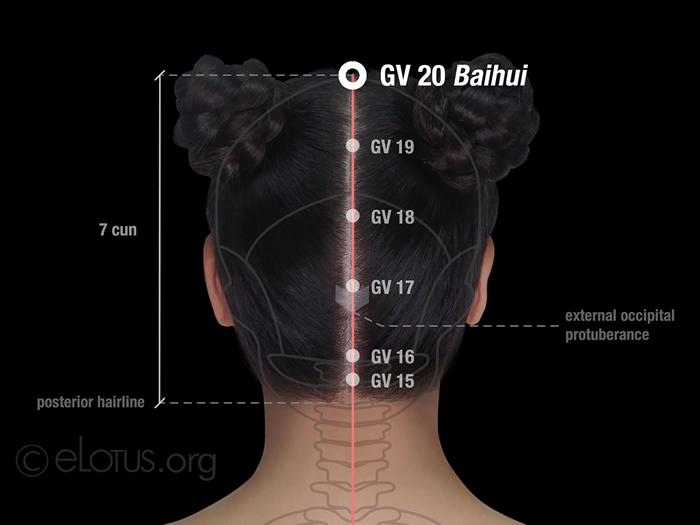
\includegraphics[width=\linewidth]{GV20_0.png}}
\newcommand{\GBLO}{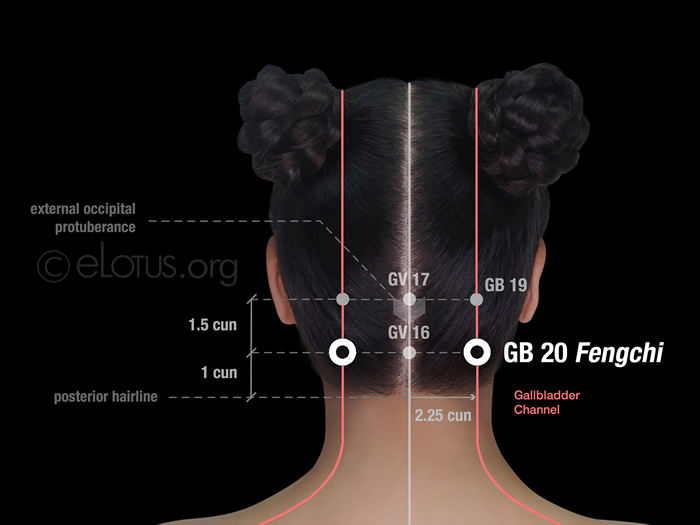
\includegraphics[width=\linewidth]{GB20.png}}
\newcommand{\STB}{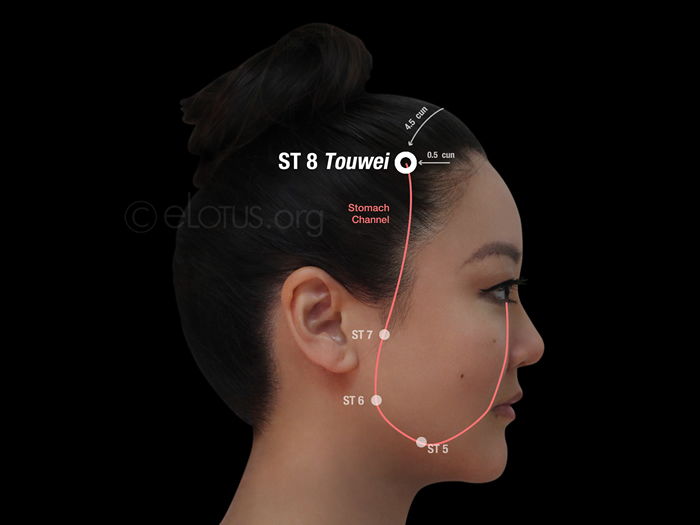
\includegraphics[width=\linewidth]{ST8.png}}
\newcommand{\GBB}{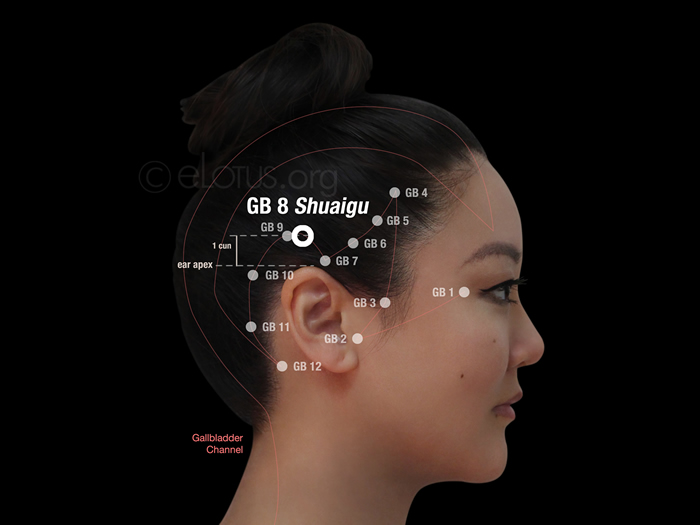
\includegraphics[width=\linewidth]{GB8.png}}
\newcommand{\ExHNS}{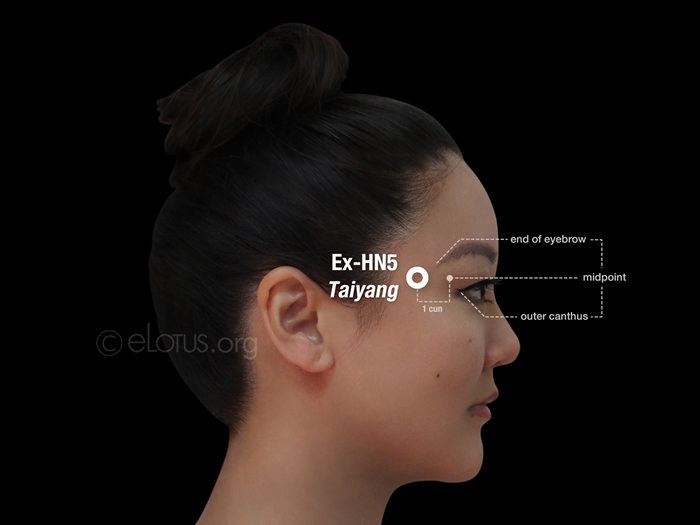
\includegraphics[width=\linewidth]{Ex-HN5.png}}
\newcommand{\AnDuong}{Ex-HN3.png}
\newcommand{\ExHNE}{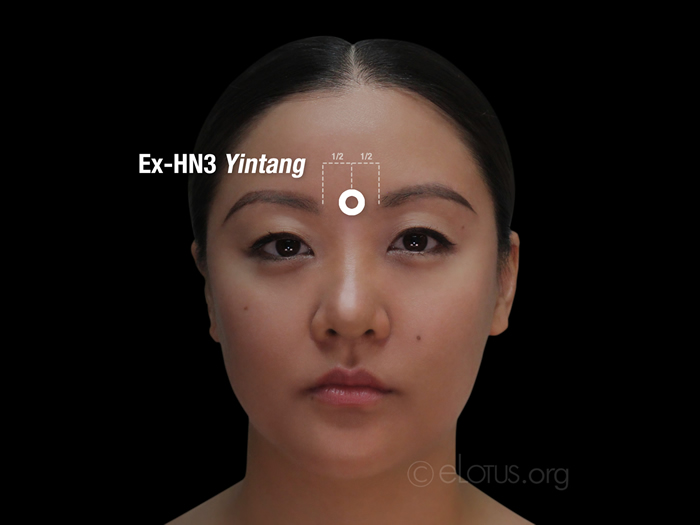
\includegraphics[width=\linewidth]{Ex-HN3.png}}
\newcommand{\BLIO}{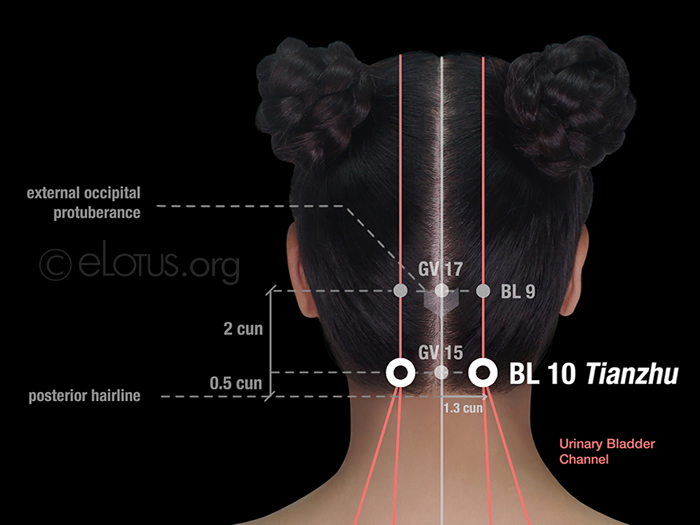
\includegraphics[width=\linewidth]{BL10.png}}
\newcommand{\GBLI}{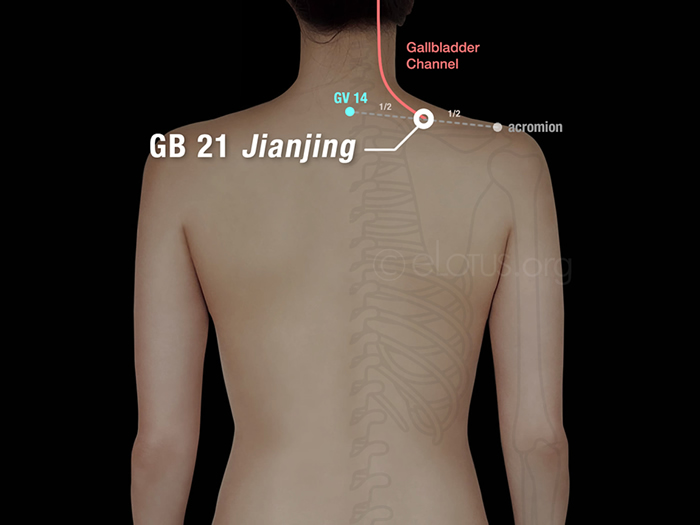
\includegraphics[width=\linewidth]{GB21.png}}
\newcommand{\LUI}{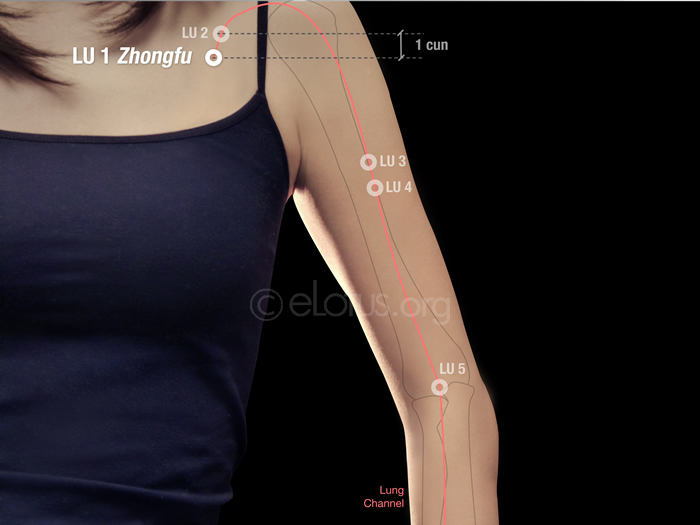
\includegraphics[width=\linewidth]{LU1.png}}
\newcommand{\BLIL}{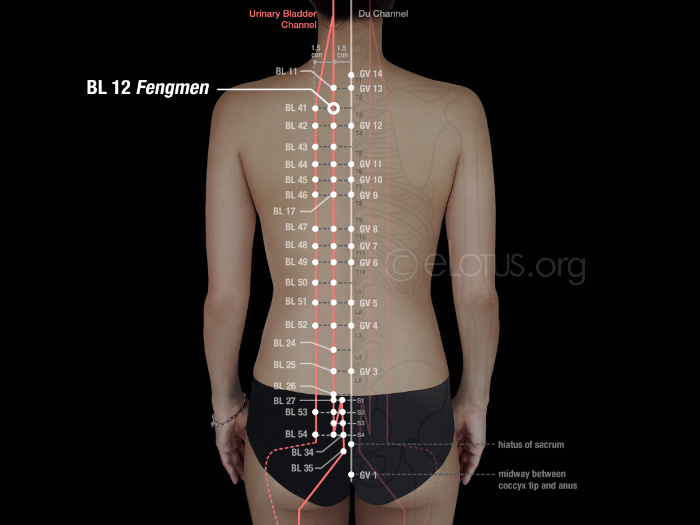
\includegraphics[width=\linewidth]{BL12.png}}
\newcommand{\LIIS}{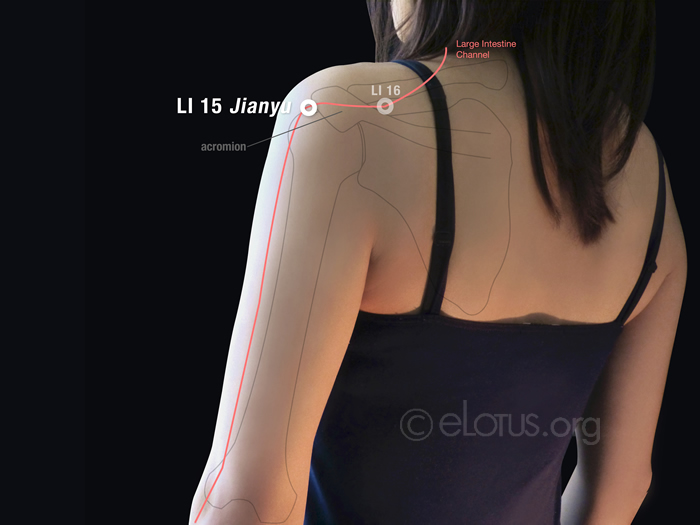
\includegraphics[width=\linewidth]{LI15b.png}}
\newcommand{\LIIC}{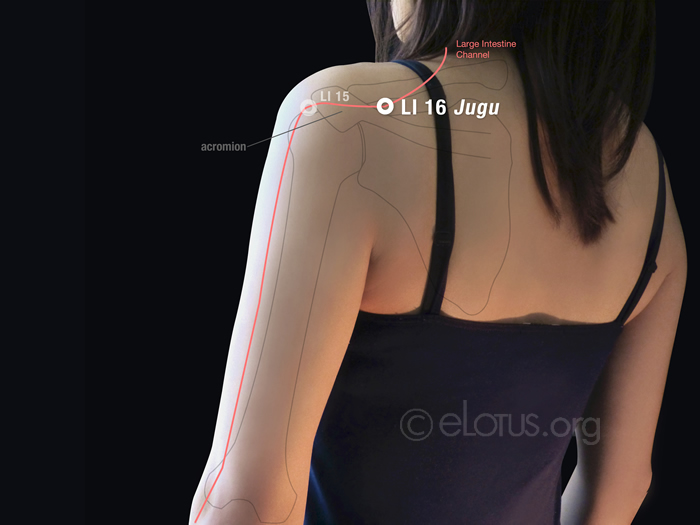
\includegraphics[width=\linewidth]{LI_16b.png}}
\newcommand{\SIIO}{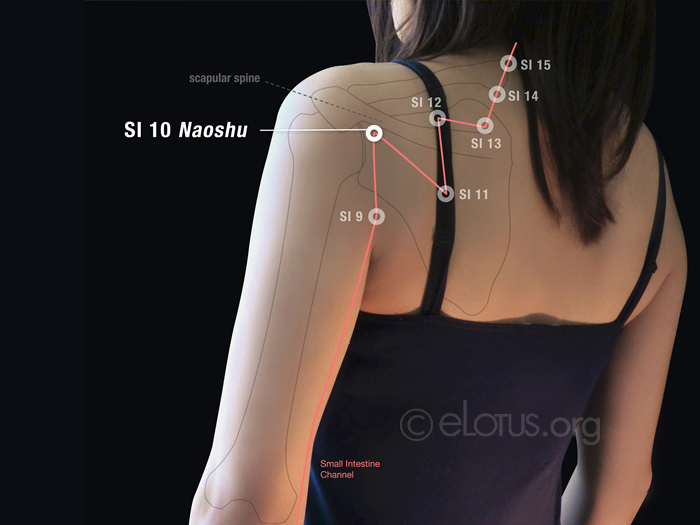
\includegraphics[width=\linewidth]{SI10.png}}
\newcommand{\SIII}{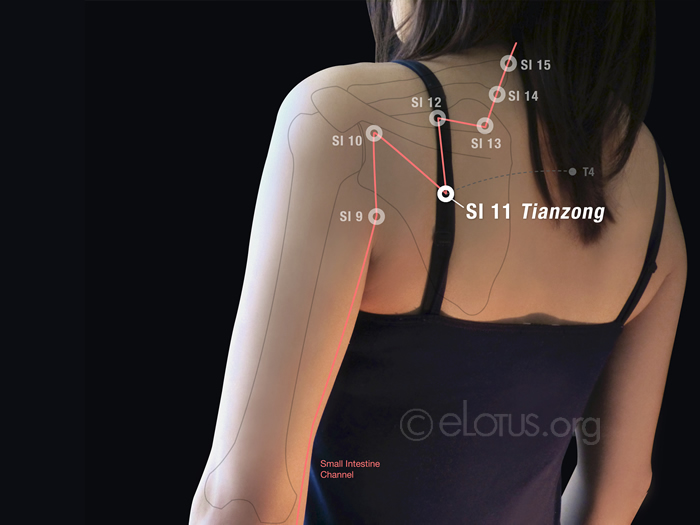
\includegraphics[width=\linewidth]{SI_11.png}}
\newcommand{\LIIA}{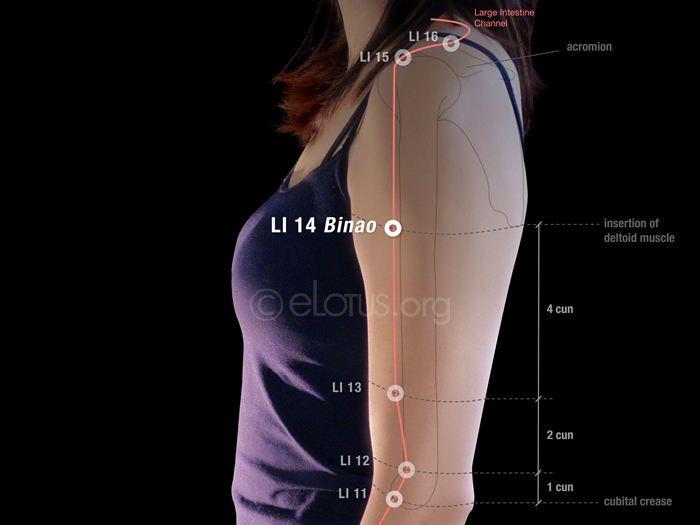
\includegraphics[width=\linewidth]{LI_14.png}}
\newcommand{\EXBL}{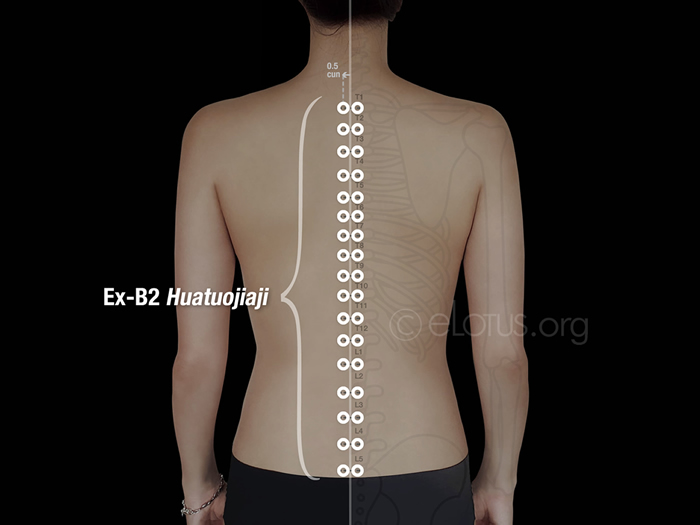
\includegraphics[width=\linewidth]{Ex_B2.png}}
\newcommand{\BLLE}{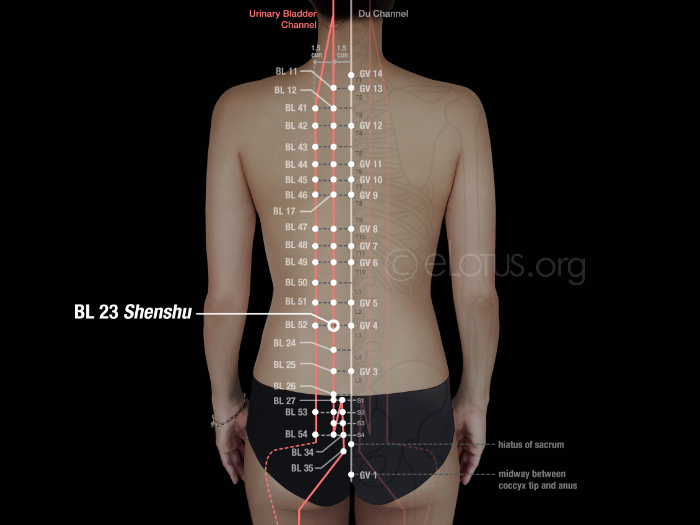
\includegraphics[width=\linewidth]{BL_23.png}}
\newcommand{\BLIT}{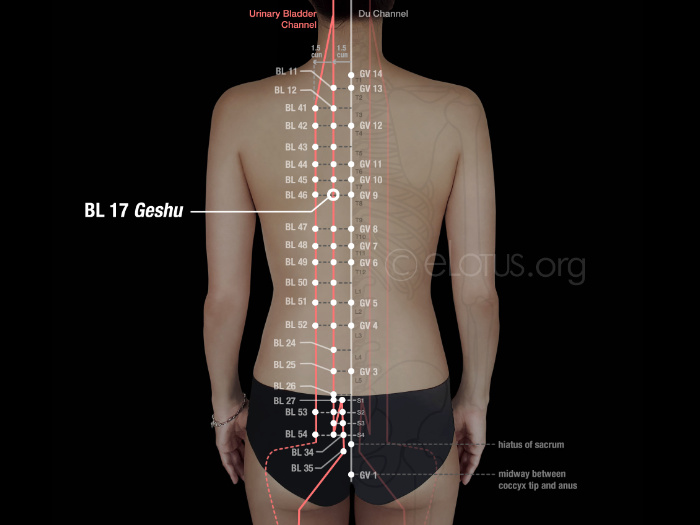
\includegraphics[width=\linewidth]{BL_17.png}}
\newcommand{\BLLS}{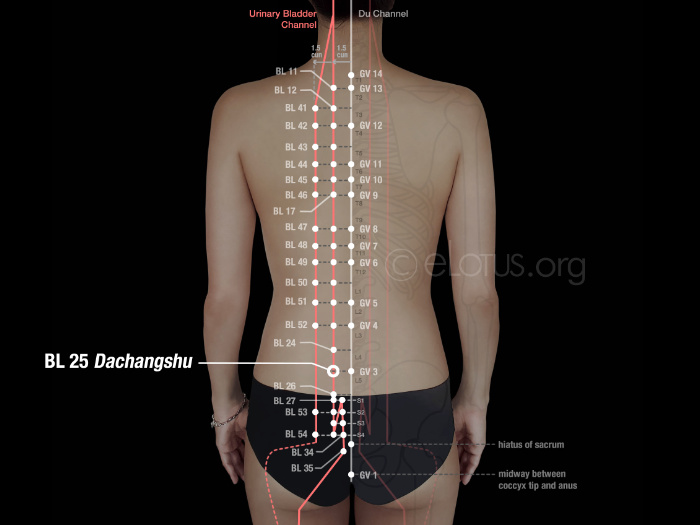
\includegraphics[width=\linewidth]{BL_25.png}}
\newcommand{\GBEO}{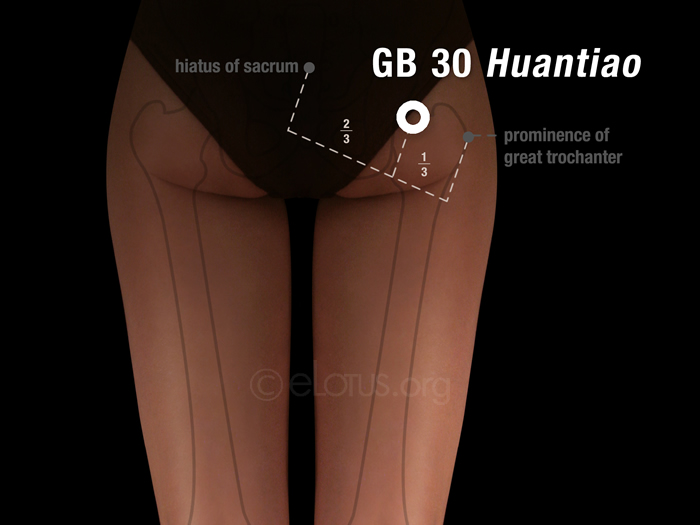
\includegraphics[width=\linewidth]{GB_30.png}}
\newcommand{\BLEC}{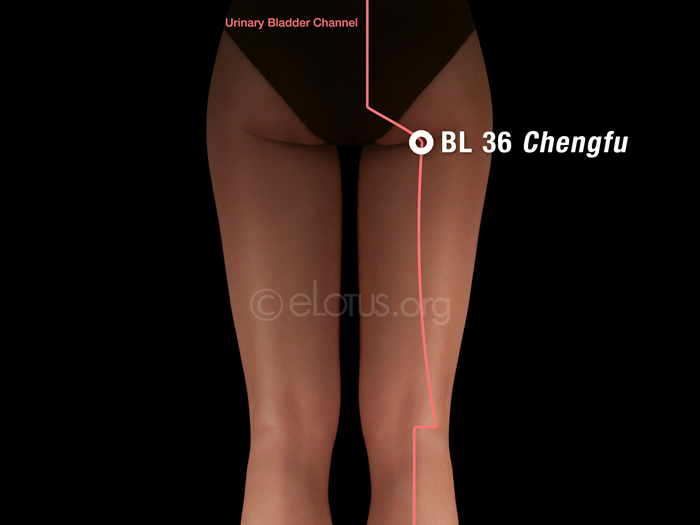
\includegraphics[width=\linewidth]{BL_36.png}}
\newcommand{\BLAO}{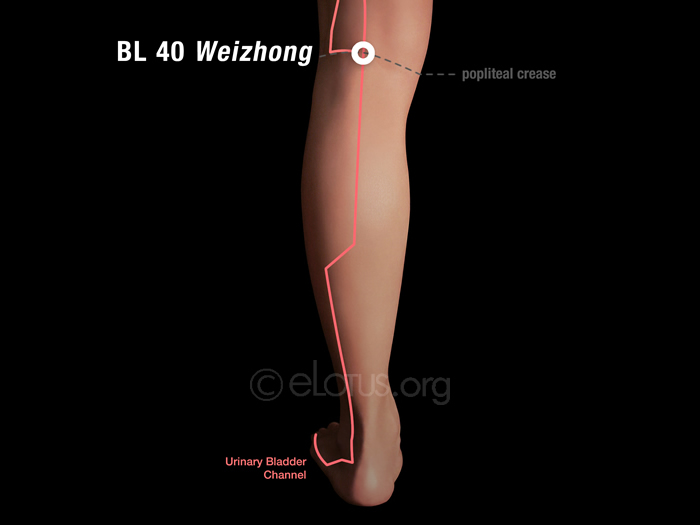
\includegraphics[width=\linewidth]{BL_40.png}}
\newcommand{\BLST}{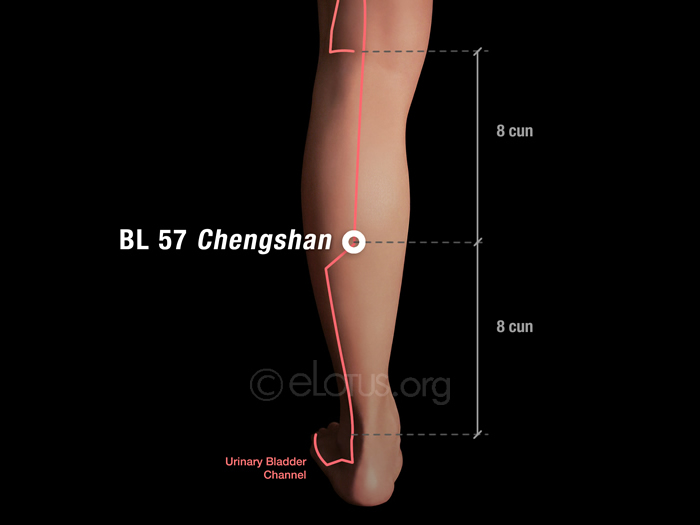
\includegraphics[width=\linewidth]{BL_57.png}}
\newcommand{\BLCO}{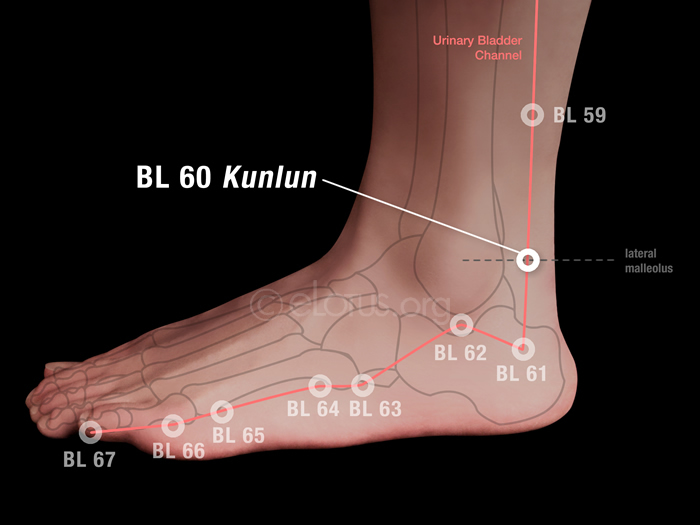
\includegraphics[width=\linewidth]{BL_60.png}}
\newcommand{\GBEI}{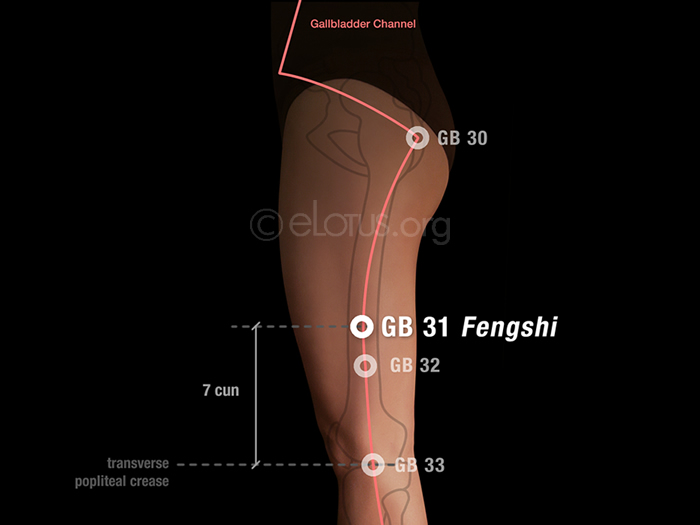
\includegraphics[width=\linewidth]{GB_31.png}}
\newcommand{\GBEA}{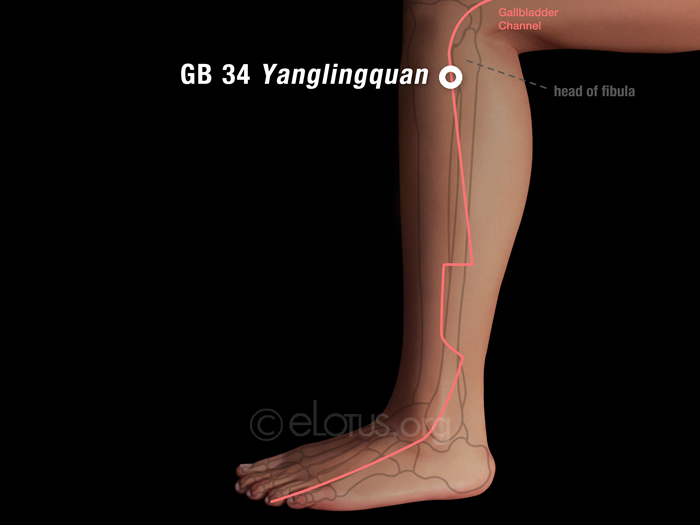
\includegraphics[width=\linewidth]{GB_34.png}}
\newcommand{\BLI}{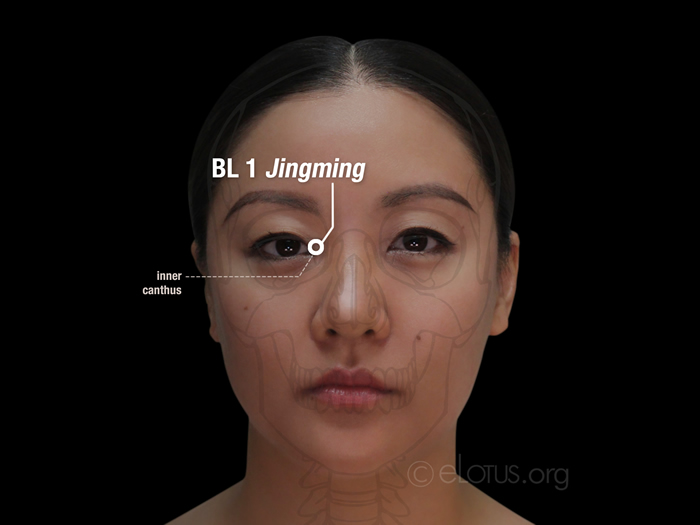
\includegraphics[width=\linewidth]{BL_1.png}}
\newcommand{\BLL}{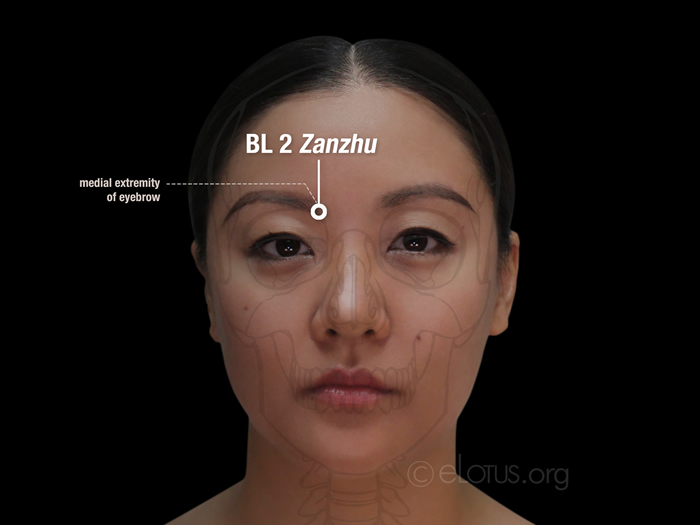
\includegraphics[width=\linewidth]{BL_2.png}}
\newcommand{\LILO}{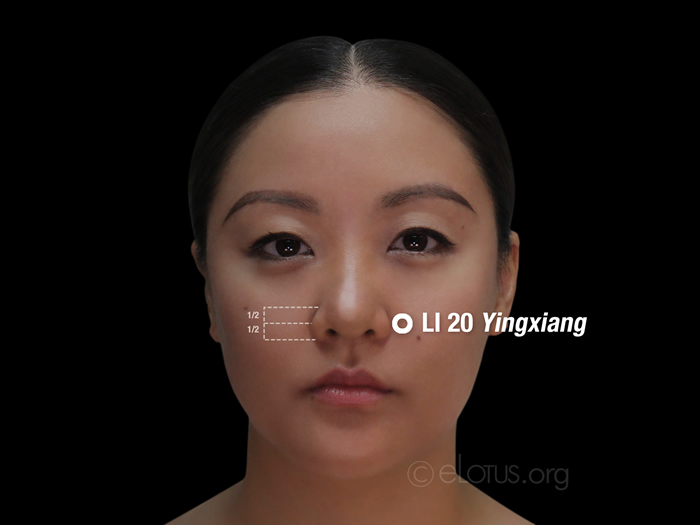
\includegraphics[width=\linewidth]{LI_20.png}}
\newcommand{\STA}{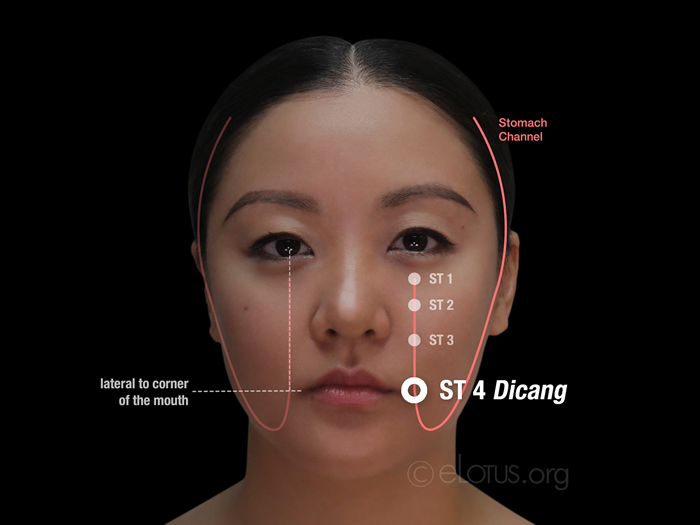
\includegraphics[width=\linewidth]{ST_4.png}}
\newcommand{\GVLC}{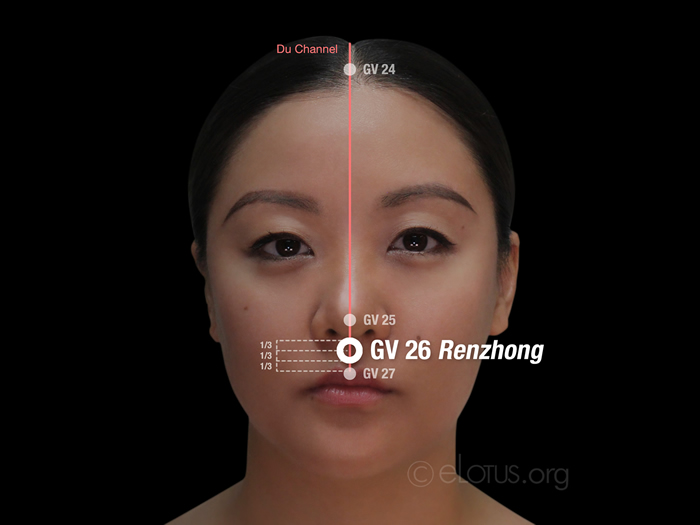
\includegraphics[width=\linewidth]{GV_26.png}}
\newcommand{\CVLA}{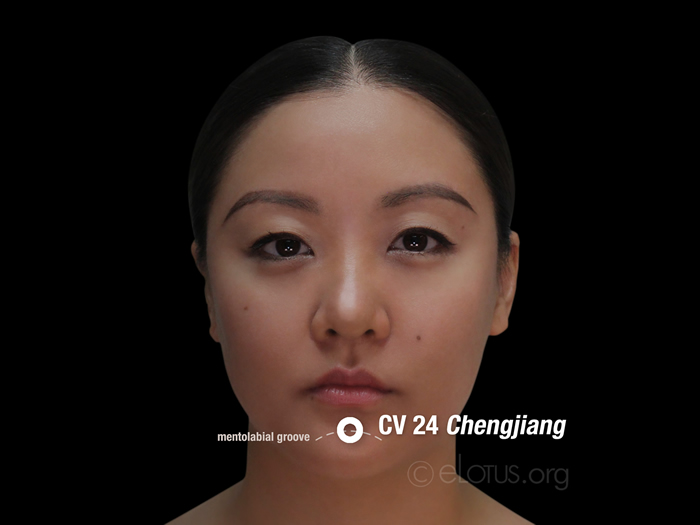
\includegraphics[width=\linewidth]{CV_24.png}}
\newcommand{\EXHNA}{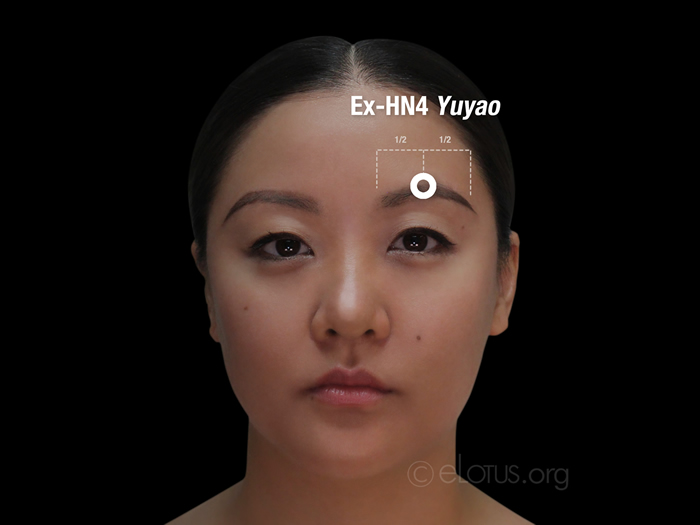
\includegraphics[width=\linewidth]{Ex_HN4.png}}
\newcommand{\LIA}{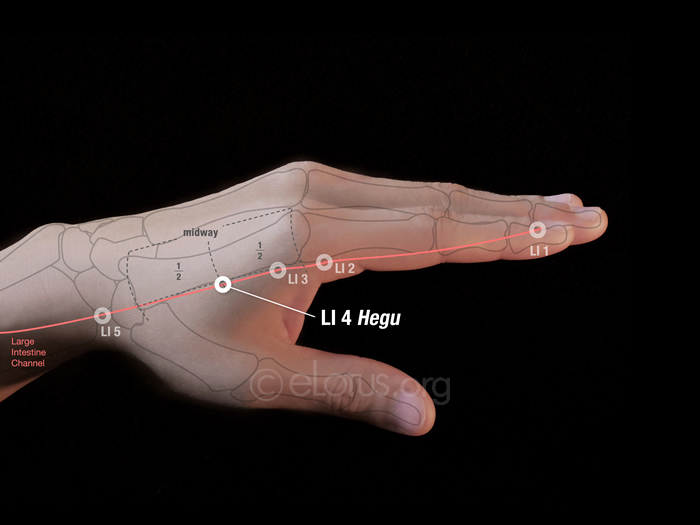
\includegraphics[width=\linewidth]{LI_4.png}}
\newcommand{\THA}{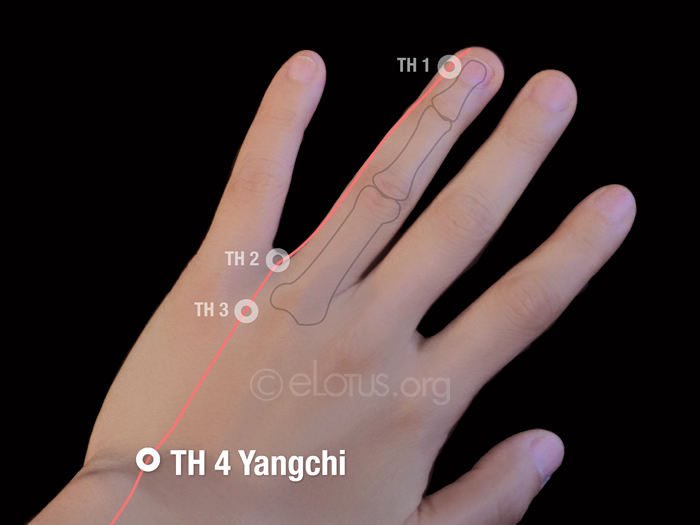
\includegraphics[width=\linewidth]{TH_4.png}}
\newcommand{\PCB}{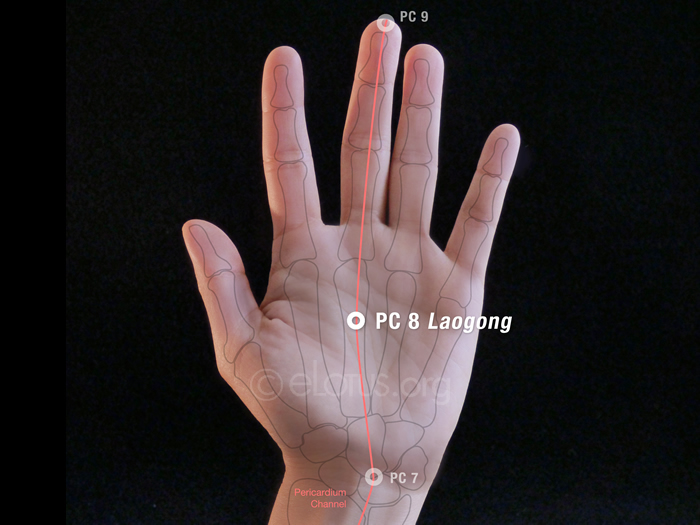
\includegraphics[width=\linewidth]{PC_8.jpg}}
\LetLtxMacro{\laogong}{\PCB}
\LetLtxMacro{\laocung}{\PCB}

\newcommand{\PCT}{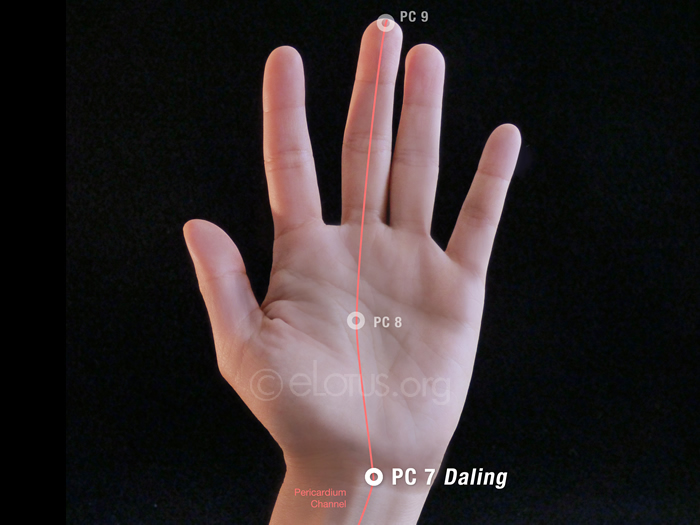
\includegraphics[width=\linewidth]{PC_7.jpg}}
\LetLtxMacro{\daling}{\PCT}
\LetLtxMacro{\dailang}{\PCT}

\newcommand{\LUIO}{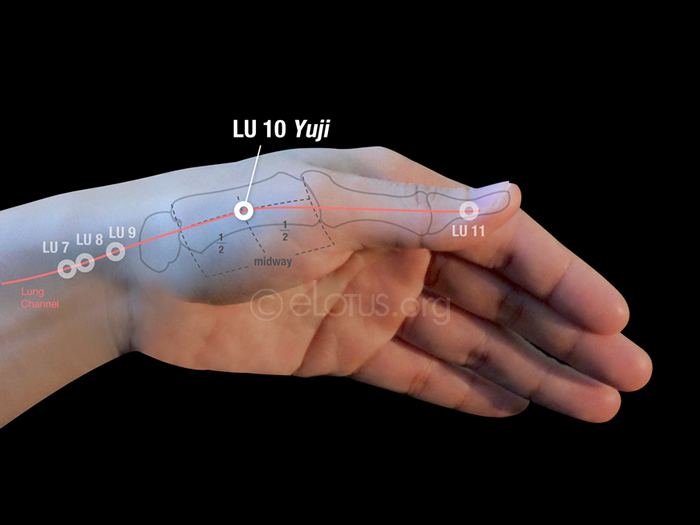
\includegraphics[width=\linewidth]{LU_10.jpg}}
\LetLtxMacro{\yuji}{\LUIO}
\LetLtxMacro{\ngute}{\LUIO}

\newcommand{\LUS}{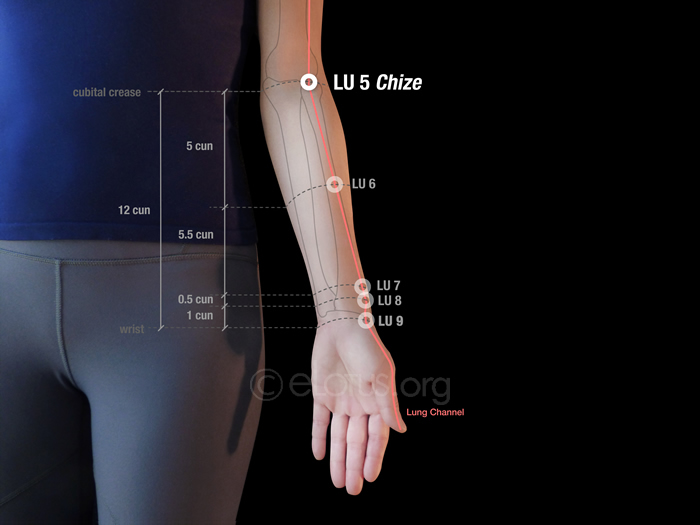
\includegraphics[width=\linewidth]{LU_5.jpg}}
\LetLtxMacro{\chize}{\LUS}
\LetLtxMacro{\xichtrach}{\LUS}

\newcommand{\LIIO}{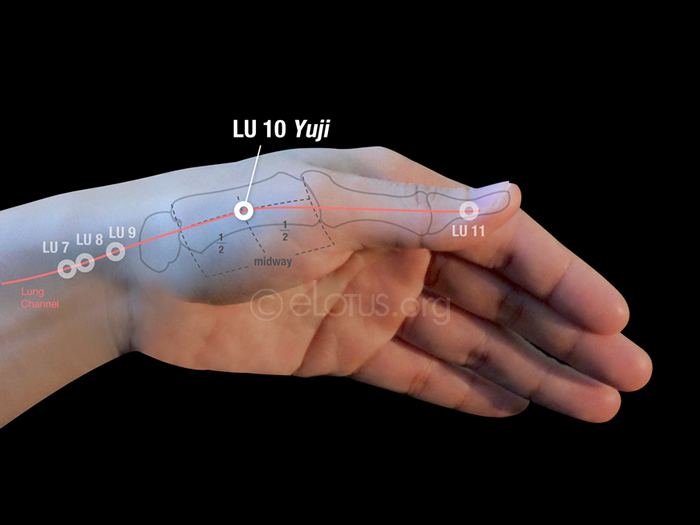
\includegraphics[width=\linewidth]{LU_10.jpg}}
\LetLtxMacro{\shousanli}{\LIIO}
\LetLtxMacro{\thutamly}{\LIIO}

\newcommand{\THS}{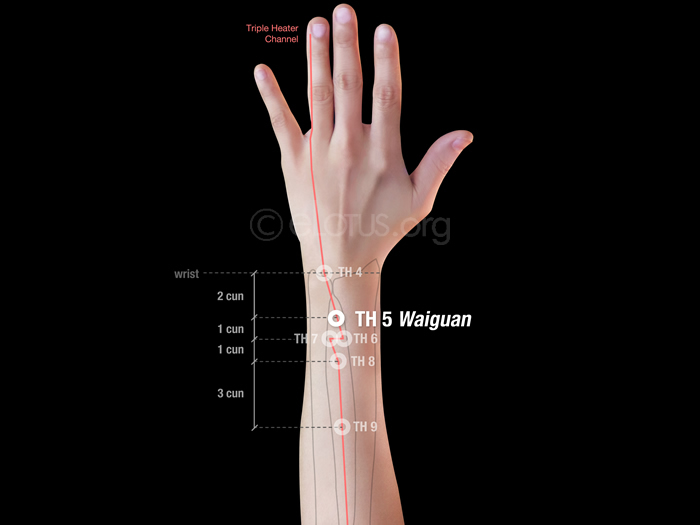
\includegraphics[width=\linewidth]{TH_5.jpg}}
\LetLtxMacro{\waiguan}{\THS}
\LetLtxMacro{\ngoaiquan}{\THS}

\newcommand{\LIII}{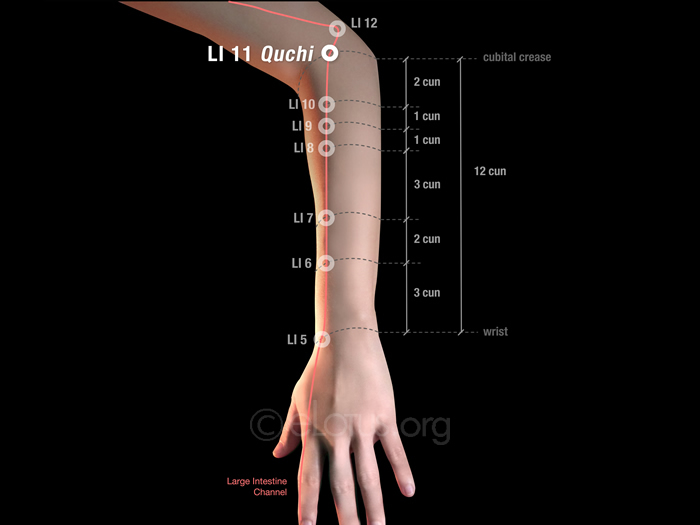
\includegraphics[width=\linewidth]{LI_11.png}}

\newcommand{\STC}{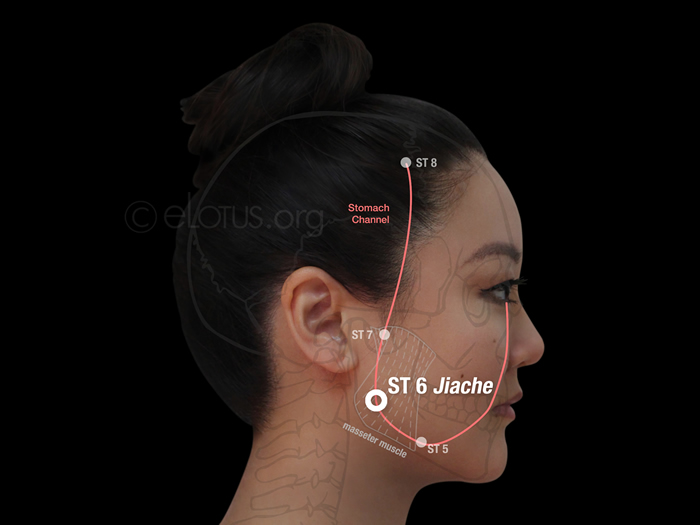
\includegraphics[width=\linewidth]{ST_6.png}}
\newcommand{\STT}{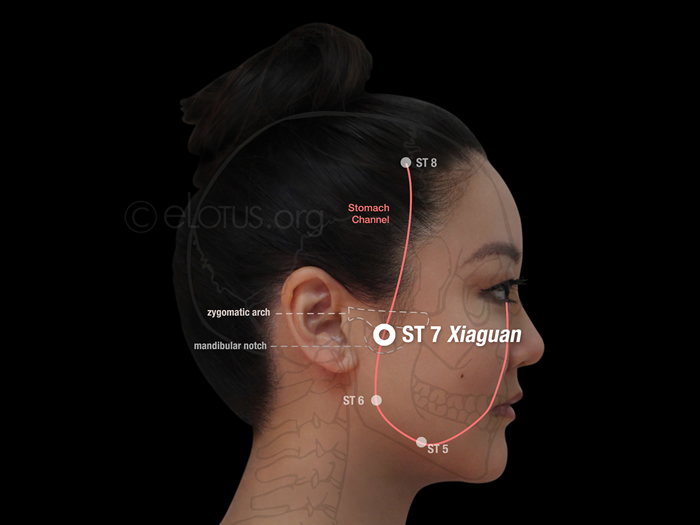
\includegraphics[width=\linewidth]{ST_7.png}}
\newcommand{\BLAE}{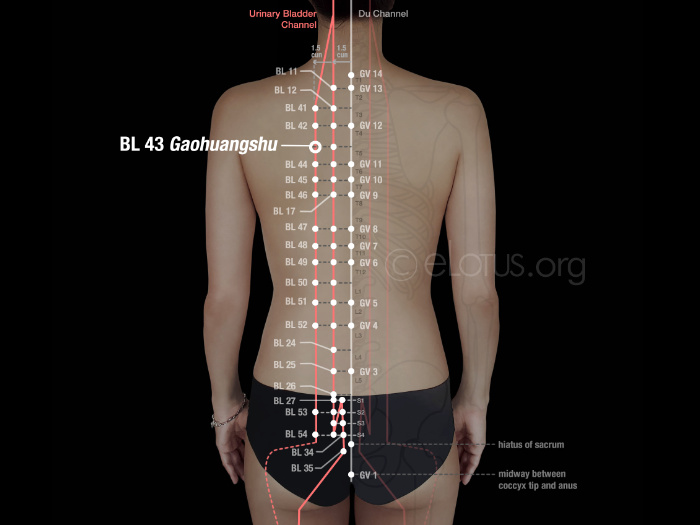
\includegraphics[width=\linewidth]{BL_43.png}}
\newcommand{\BLET}{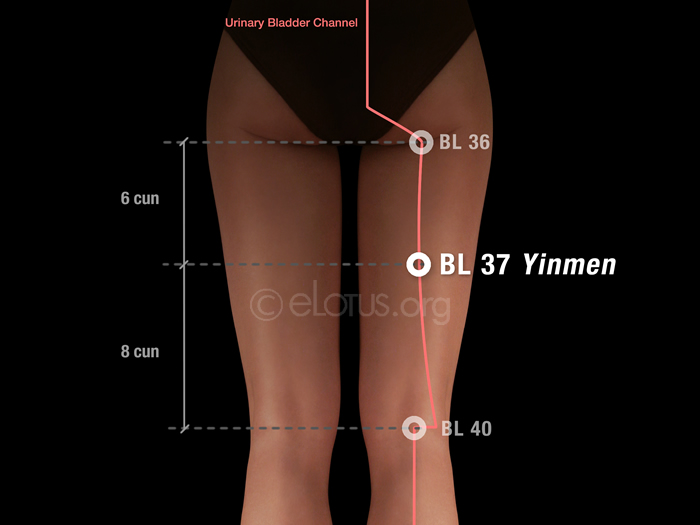
\includegraphics[width=\linewidth]{BL_37.png}}
\newcommand{\GBEG}{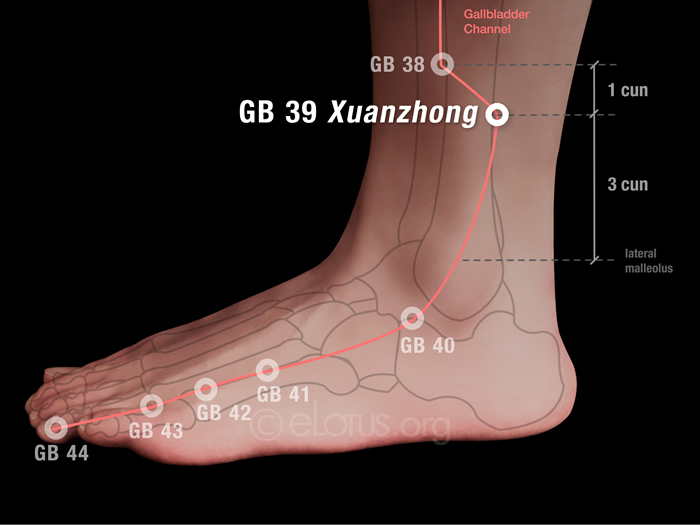
\includegraphics[width=\linewidth]{GB_39.png}}
\newcommand{\STAI}{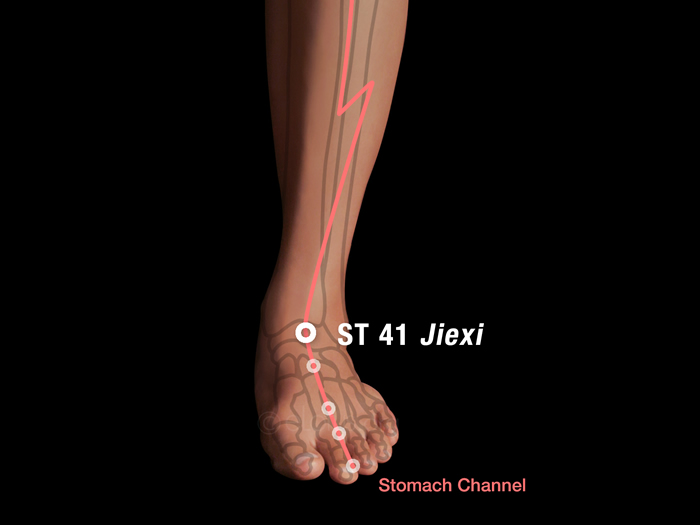
\includegraphics[width=\linewidth]{ST_41.png}}
\newcommand{\HTT}{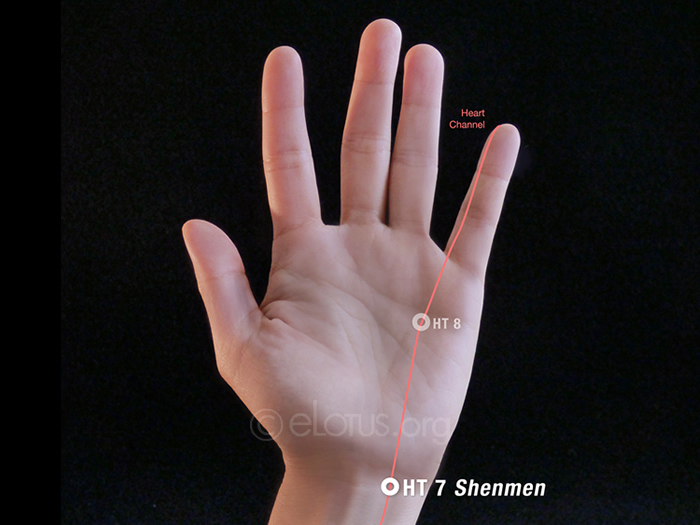
\includegraphics[width=\linewidth]{HT_7a.png}}
\newcommand{\KII}{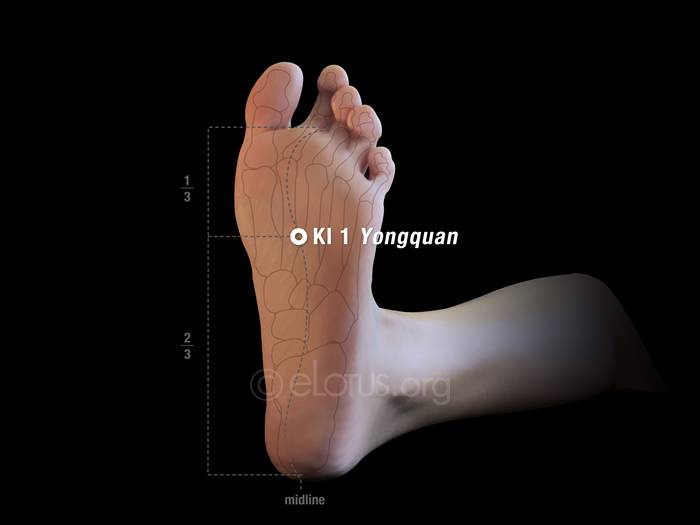
\includegraphics[width=\linewidth]{KI_1.png}}
\newcommand{\PCC}{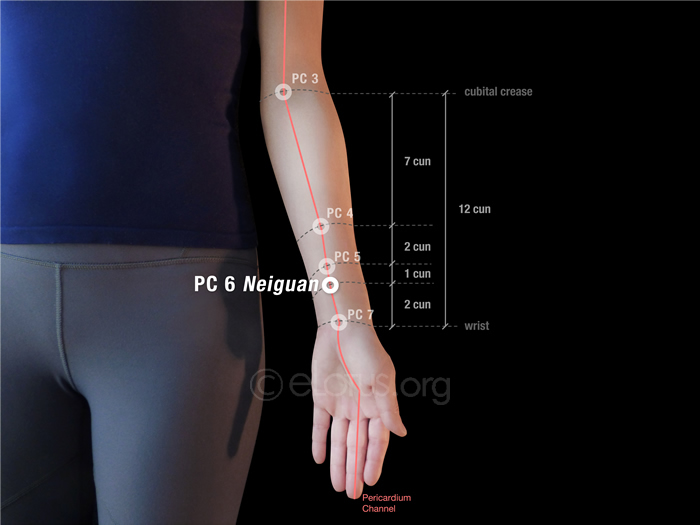
\includegraphics[width=\linewidth]{PC_6.png}}
\newcommand{\SPC}{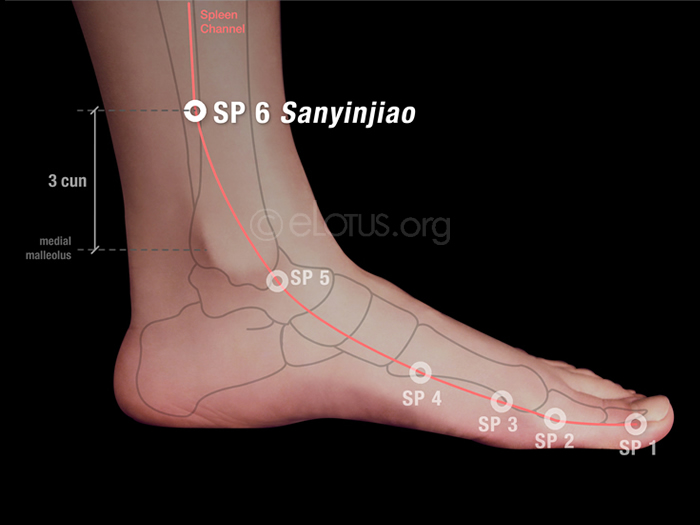
\includegraphics[width=\linewidth]{SP_6.png}}

\newcommand{\GBIA}{\includegraphics[width=\linewidth]{"GB 14.jpg"}}
\LetLtxMacro{\yangbai}{\GBIA}
\LetLtxMacro{\duongbach}{\GBIA}

\newcommand{\HNI}{\includegraphics[width=\linewidth]{"HN1.jpg"}}
\LetLtxMacro{\sishencong}{\HNI}
\LetLtxMacro{\tuthanthong}{\HNI}

\newcommand{\GBA}{\includegraphics[width=\linewidth]{"GB 4.jpg"}}
\LetLtxMacro{\hanyan}{\GBA}
\LetLtxMacro{\hamyen}{\GBA}

\newcommand{\GVIC}{\includegraphics[width=\linewidth]{"GV16.jpg"}}
\LetLtxMacro{\fengfu}{\GVIC}
\LetLtxMacro{\phongphu}{\GVIC}

\newcommand{\SIIT}{\includegraphics[width=\linewidth]{"SI 17.jpg"}}
\LetLtxMacro{\thiendung}{\SIIT}
\LetLtxMacro{\tianrong}{\SIIT}

\newcommand{\EXHNIS}{\includegraphics[width=\linewidth]{"Ex-HN15.jpg"}}
\LetLtxMacro{\bachlao}{\EXHNIS}
\LetLtxMacro{\jingbailao}{\EXHNIS}


\newcommand{\BLIE}{\includegraphics[width=\linewidth]{"Ex-HN15.jpg"}}
\LetLtxMacro{\phedu}{\BLIE}
\LetLtxMacro{\feishu}{\BLIE}


\newcommand{\BLIA}{\includegraphics[width=\linewidth]{"BL_14.jpg"}}
\LetLtxMacro{\quyetamdu}{\BLIA}
\LetLtxMacro{\jueyinshu}{\BLIA}


\newcommand{\BLIC}{\includegraphics[width=\linewidth]{"BL_16.jpg"}}
\LetLtxMacro{\docdu}{\BLIC}
\LetLtxMacro{\dushu}{\BLIC}

\newcommand{\SIG}{\includegraphics[width=\linewidth]{"SI_9.jpg"}}
\LetLtxMacro{\kientrinh}{\SIG}
\LetLtxMacro{\jianzhen}{\SIG}

\LetLtxMacro{\geshu}{\BLIT}

\newcommand{\BLIB}{\includegraphics[width=\linewidth]{"BL_18.jpg"}}
\LetLtxMacro{\candu}{\BLIB}
\LetLtxMacro{\canshu}{\BLIB}

\newcommand{\BLIG}{\includegraphics[width=\linewidth]{"BL_19.jpg"}}
\LetLtxMacro{\domdu}{\BLIG}

\newcommand{\BLLO}{\includegraphics[width=\linewidth]{"BL_20.jpg"}}
\LetLtxMacro{\tidu}{\BLLO}

\newcommand{\BLLI}{\includegraphics[width=\linewidth]{"BL_21.jpg"}}
\LetLtxMacro{\vidu}{\BLLI}


\newcommand{\BLLL}{\includegraphics[width=\linewidth]{"BL_22.jpg"}}
\LetLtxMacro{\tamtieudu}{\BLLL}

\newcommand{\KIE}{\includegraphics[width=\linewidth]{"KI_3.jpg"}}
\LetLtxMacro{\taixi}{\KIE}
\LetLtxMacro{\thaikhe}{\KIE}


\newcommand{\BLSA}{\includegraphics[width=\linewidth]{"BL_54.jpg"}}
\LetLtxMacro{\zhibian}{\BLSA}
\LetLtxMacro{\tratbien}{\BLSA}

\newcommand{\STAO}{\includegraphics[width=\linewidth]{"ST_40.jpg"}}
\LetLtxMacro{\fenglong}{\STAO}
\LetLtxMacro{\phonglong}{\STAO}


\newcommand{\STEC}{\includegraphics[width=\linewidth]{"ST_36.jpg"}}
\LetLtxMacro{\zusanli}{\STEC}
\LetLtxMacro{\tuctamly}{\STEC}


\newcommand{\EXLEIO}{\includegraphics[width=\linewidth]{"Ex-LE10_0.jpg"}}
\LetLtxMacro{\batphong}{\EXLEIO}
\LetLtxMacro{\bafeng}{\EXLEIO}


\newcommand{\LRE}{\includegraphics[width=\linewidth]{"LR_3.jpg"}}
\LetLtxMacro{\taichong}{\LRE}
\LetLtxMacro{\thaixung}{\LRE}


\newcommand{\STAA}{\includegraphics[width=\linewidth]{"ST_44.jpg"}}
\LetLtxMacro{\neiting}{\STAA}
\LetLtxMacro{\noidinh}{\STAA}


\newcommand{\STES}{\includegraphics[width=\linewidth]{"ST_35.jpg"}}
\LetLtxMacro{\docty}{\STES}
\LetLtxMacro{\dubi}{\STES}


\newcommand{\EXLES}{\includegraphics[width=\linewidth]{"Ex-LE5.jpg"}}
\LetLtxMacro{\xiyan}{\EXLES}
\LetLtxMacro{\tatnhan}{\EXLES}

\newcommand{\EXLEL}{\includegraphics[width=\linewidth]{"Ex-LE2.jpg"}}
\LetLtxMacro{\heding}{\EXLEL}
\LetLtxMacro{\hacdinh}{\EXLEL}


\newcommand{\SPIO}{\includegraphics[width=\linewidth]{"SP_10a.jpg"}}
\LetLtxMacro{\huyethai}{\SPIO}
\LetLtxMacro{\xuehai}{\SPIO}


\newcommand{\STEA}{\includegraphics[width=\linewidth]{"ST_34.jpg"}}
\LetLtxMacro{\liangqiu}{\STEA}
\LetLtxMacro{\luongkhau}{\STEA}


% \newcommand{\BLLE}{\includegraphics[width=\linewidth]{"BL_23.jpg"}}
% \LetLtxMacro{\thandu}{\BLLE}

\newcommand{\BLLA}{\includegraphics[width=\linewidth]{"BL_24.jpg"}}
\LetLtxMacro{\khihaidu}{\BLLA}


% \newcommand{\BLLS}{\includegraphics[width=\linewidth]{"BL_25.jpg"}}
% \LetLtxMacro{\daitruongdu}{\BLLS}

\newcommand{\BLLC}{\includegraphics[width=\linewidth]{"BL_26.jpg"}}
\LetLtxMacro{\quannguyendu}{\BLLC}


\newcommand{\BLLT}{\includegraphics[width=\linewidth]{"BL_27.jpg"}}
\LetLtxMacro{\tieutruongdu}{\BLLT}


\newcommand{\EXBT}{\includegraphics[width=\linewidth]{"Ex-B7.jpg"}}
\LetLtxMacro{\yeunhan}{\EXBT}


\newcommand{\thanmon}{\HTT}
\newcommand{\dungtuyen}{\KII}
\newcommand{\noiquan}{\PCC}
\newcommand{\tamamgiao}{\SPC}
\newcommand{\anmon}{\BLET}
\newcommand{\huyenchung}{\GBEG}
\newcommand{\giaikhe}{\STAI}

\newcommand{\caohoang}{\BLAE}
\newcommand{\khuctri}{\LIII}
\newcommand{\hopcoc}{\LIA}
\newcommand{\duongtri}{\THA}

\newcommand{\nguyeu}{\EXHNA}

\newcommand{\giapxa}{\STC}
\newcommand{\haquan}{\STT}

\newcommand{\nhantrung}{\GVLC}
\newcommand{\thuatuong}{\CVLA}

\newcommand{\nghinhduong}{\LILO}
\newcommand{\nghinhhuong}{\LILO}
\newcommand{\diathuong}{\STA}
\newcommand{\toantruc}{\BLL}
\newcommand{\tinhminh}{\BLI}
\newcommand{\hoankhieu}{\GBEO}
\newcommand{\thuaphu}{\BLEC}
\newcommand{\uytrung}{\BLAO}
\newcommand{\thuason}{\BLST}
\newcommand{\conlon}{\BLCO}

\newcommand{\kienngung}{\LIIS}
\newcommand{\thaiduong}{\ExHNS}
\newcommand{\anduong}{\ExHNE}
\newcommand{\dauduy}{\STB}
\newcommand{\phongtri}{\GBLO}
\newcommand{\bachhoi}{\GVLO}
\newcommand{\xuatcoc}{\GBB}
\newcommand{\thientru}{\BLIO}
\newcommand{\kientinh}{\GBLI}
\newcommand{\phongmon}{\BLIL}
\newcommand{\trungphu}{\LUI}
\newcommand{\nhudu}{\SIIO}
\newcommand{\cucot}{\LIIC}
\newcommand{\thientong}{\SIII}
\newcommand{\tinhu}{\LIIA}
\newcommand{\giaptich}{\EXBL}
\newcommand{\thandu}{\BLLE}
\newcommand{\cachdu}{\BLIT}
\newcommand{\daitruongdu}{\BLLS}

\newcommand{\phongthi}{\GBEI}
\newcommand{\duonglangtuyen}{\GBEA}

\newcommand{\codelta}{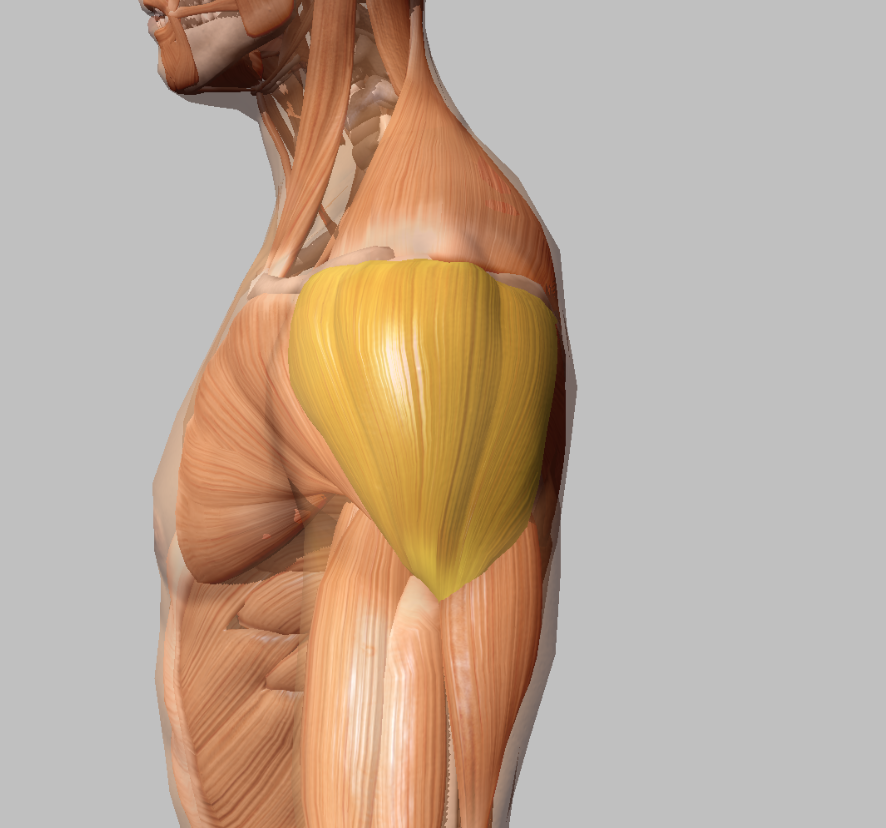
\includegraphics[width=\linewidth]{codelta.png}}


\newcommand{\omout}{ 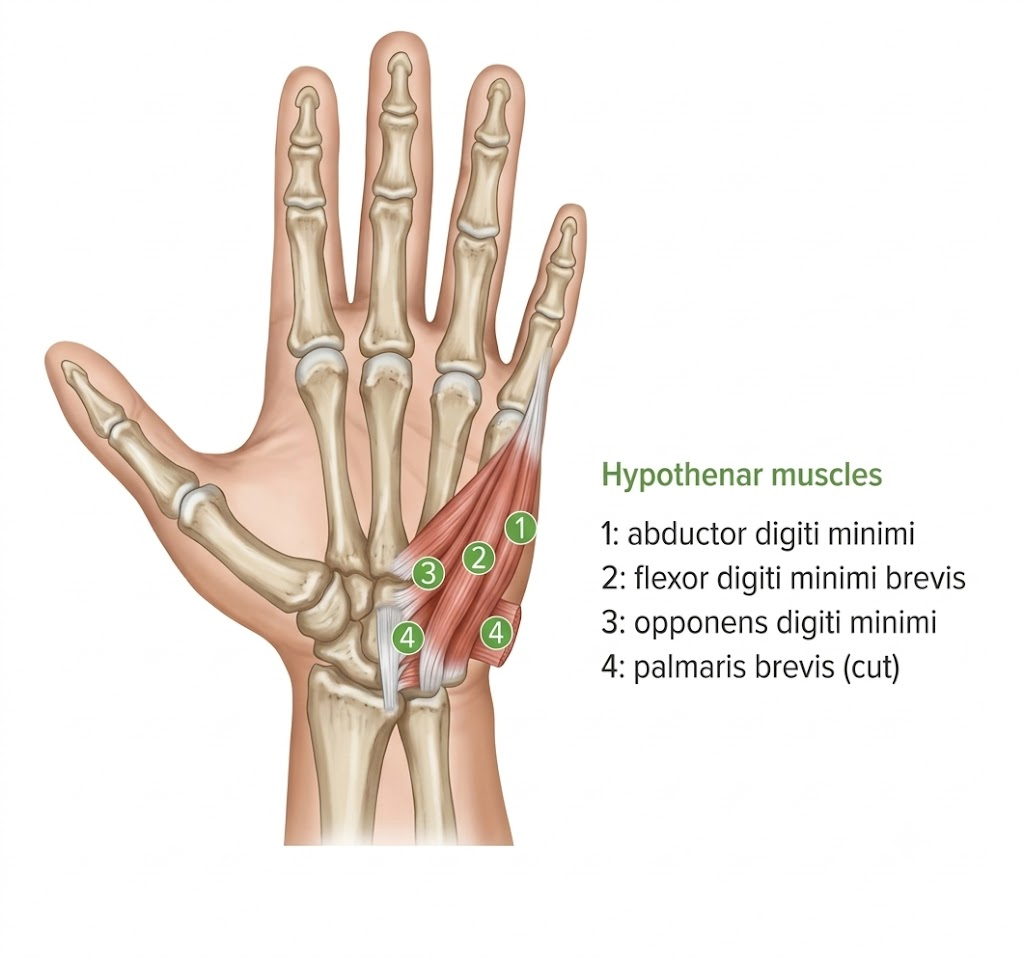
\includegraphics[width=1cm]{omout.png}}

\newcommand{\xoa}{\href{https://youtu.be/t8xlblzjSB0}{Xoa}}
\newcommand{\xat}{\href{https://youtu.be/5LxNXUudT0I}{Xát}}
\newcommand{\miet}{\href{https://youtu.be/C9047VbZbUE}{Miết}}
\newcommand{\phanhop}{\href{https://youtu.be/U7U3X2HWl14}{Phân hợp}}
\newcommand{\veo}{\href{https://youtu.be/Pooxu3bt3PU}{Véo}}
\newcommand{\vo}{\href{https://youtu.be/jX2Qz3dG_Fc}{Vỗ}}

\newcommand{\acday}{\href{https://youtu.be/BW-4i2ZW-V8}{Day}}
\newcommand{\dam}{\href{https://youtu.be/py1QDphCHxo}{Đấm}}
\newcommand{\chat}{\href{https://youtu.be/lzffl4TgL-I}{Chặt}}
\newcommand{\lan}{\href{https://youtu.be/2GyB6WE_xA4}{Lăn}}
\newcommand{\bop}{\href{https://youtu.be/ysqOetYi-L0}{Bóp}}
\newcommand{\von}{\href{}{Vờn}}

\newcommand{\cui}{\href{https://youtu.be/PqQY7ha7lAE}{Cúi}}
\newcommand{\ngua}{\href{https://youtu.be/aRl4YCO2omE}{Ngửa}}
\newcommand{\xoayphai}{\href{https://youtu.be/t8waFWkFmwU}{Xoay phải}}
\newcommand{\xoaytrai}{\href{https://youtu.be/urWJf_bhbUQ}{Xoay trái}}
\newcommand{\nhiengphai}{\href{https://youtu.be/noAQqTXWMBQ}{Nghiêng phải}}
\newcommand{\nhiengtrai}{\href{https://youtu.be/xn3b8cdrlU0}{Nghiêng trái}}
\newcommand{\xoayhonhop}{\href{https://youtu.be/S34xJ21dV3o}{Xoay hỗn hợp}}

\newcommand{\vandongco}{
Một tay để ở cằm, một tay để ở vùng chẩm. Hai tay vận động ngược chiều nhau một cách nhẹ nhàng, sau đó đột nhiên làm mạnh một cái sẽ phát ra tiếng kêu khục, rồi đổi chiều làm phía bên kia.

Khi vận động cổ cần chú ý bảo bệnh nhân để tự nhiên không chống đỡ (lên gân, rụt cổ lại). Nếu bệnh nhân có phản xạ chống đỡ thì vừa làm vừa nói chuyện với bệnh nhân, nếu thấy nhẹ dưới tay phải tranh thủ vận động cổ ngay.
}

\newcommand{\mbu}{\
Vận động cột sống tư thế nằm sấp bài ưỡn cột sống và thắt lưng cùng.\
Một tay đặt ở lưng dưới, tay còn lại ôm đầu gối (đùi dưới) bệnh nhân.\
Nâng đầu gối lên.\
}

\newcommand{\mfgd}{\
Vận động cột sống.\
Tư thế nằm ngửa.\
Một tay cầm cổ chân tay còn lại đặt lên đầu gối phía dưới.\
Đẩy đầu gối lên ngực kết hợp với xoay tròn.\
Sau đó hạ đầu gối về tư thế chuẩn bị.\
}

\newcommand{\mfvx}{\
Vận động cột sống.\
Tư thế nằm ngửa.\
Để bệnh nhân vào tư thế co chân vào bụng.\
Cánh tay dưới của một tay để ở đầu gối trên,
cánh tay dưới của tay còn lại để ở gần cổ chân.
Lòng bàn tay ôm xát mặt ngoài chân.
Đầu ngón tay có thể chạm vào đùi bệnh nhân.
Ghì xuống sao cho đốt thắt lưng cùng của bệnh nhân được giải phóng khỏi đệm.
Thực hiện xoay.
Chú ý hai đầu gối phải thẳng.\
}

\newcommand{\mfvgd}{\
Vận động cột sống.
Tư thế nằm ngửa.

Để bệnh nhân vào tư thế co chân vào bụng.\
Cánh tay dưới của một tay để ở đầu gối trên,
cánh tay dưới của tay còn lại để ở cạnh mông.

Nâng mông bệnh nhân lên\
}

% \includeonly{sections/basic_therapy.tex}
% \includeonly{sections/manipulation.tex}
% \includeonly{sections/therapy.tex}
% \includeonly{sections/acupuncture_points.tex}
% \includeonly{sections/qigong.tex}

\begin{document}
\keepXColumns

\begin{titlepage}
    % Lệnh chèn ảnh nền phủ toàn bộ trang bìa
    \AddToShipoutPictureBG*{
        \AtPageLowerLeft{
            \transparent{1}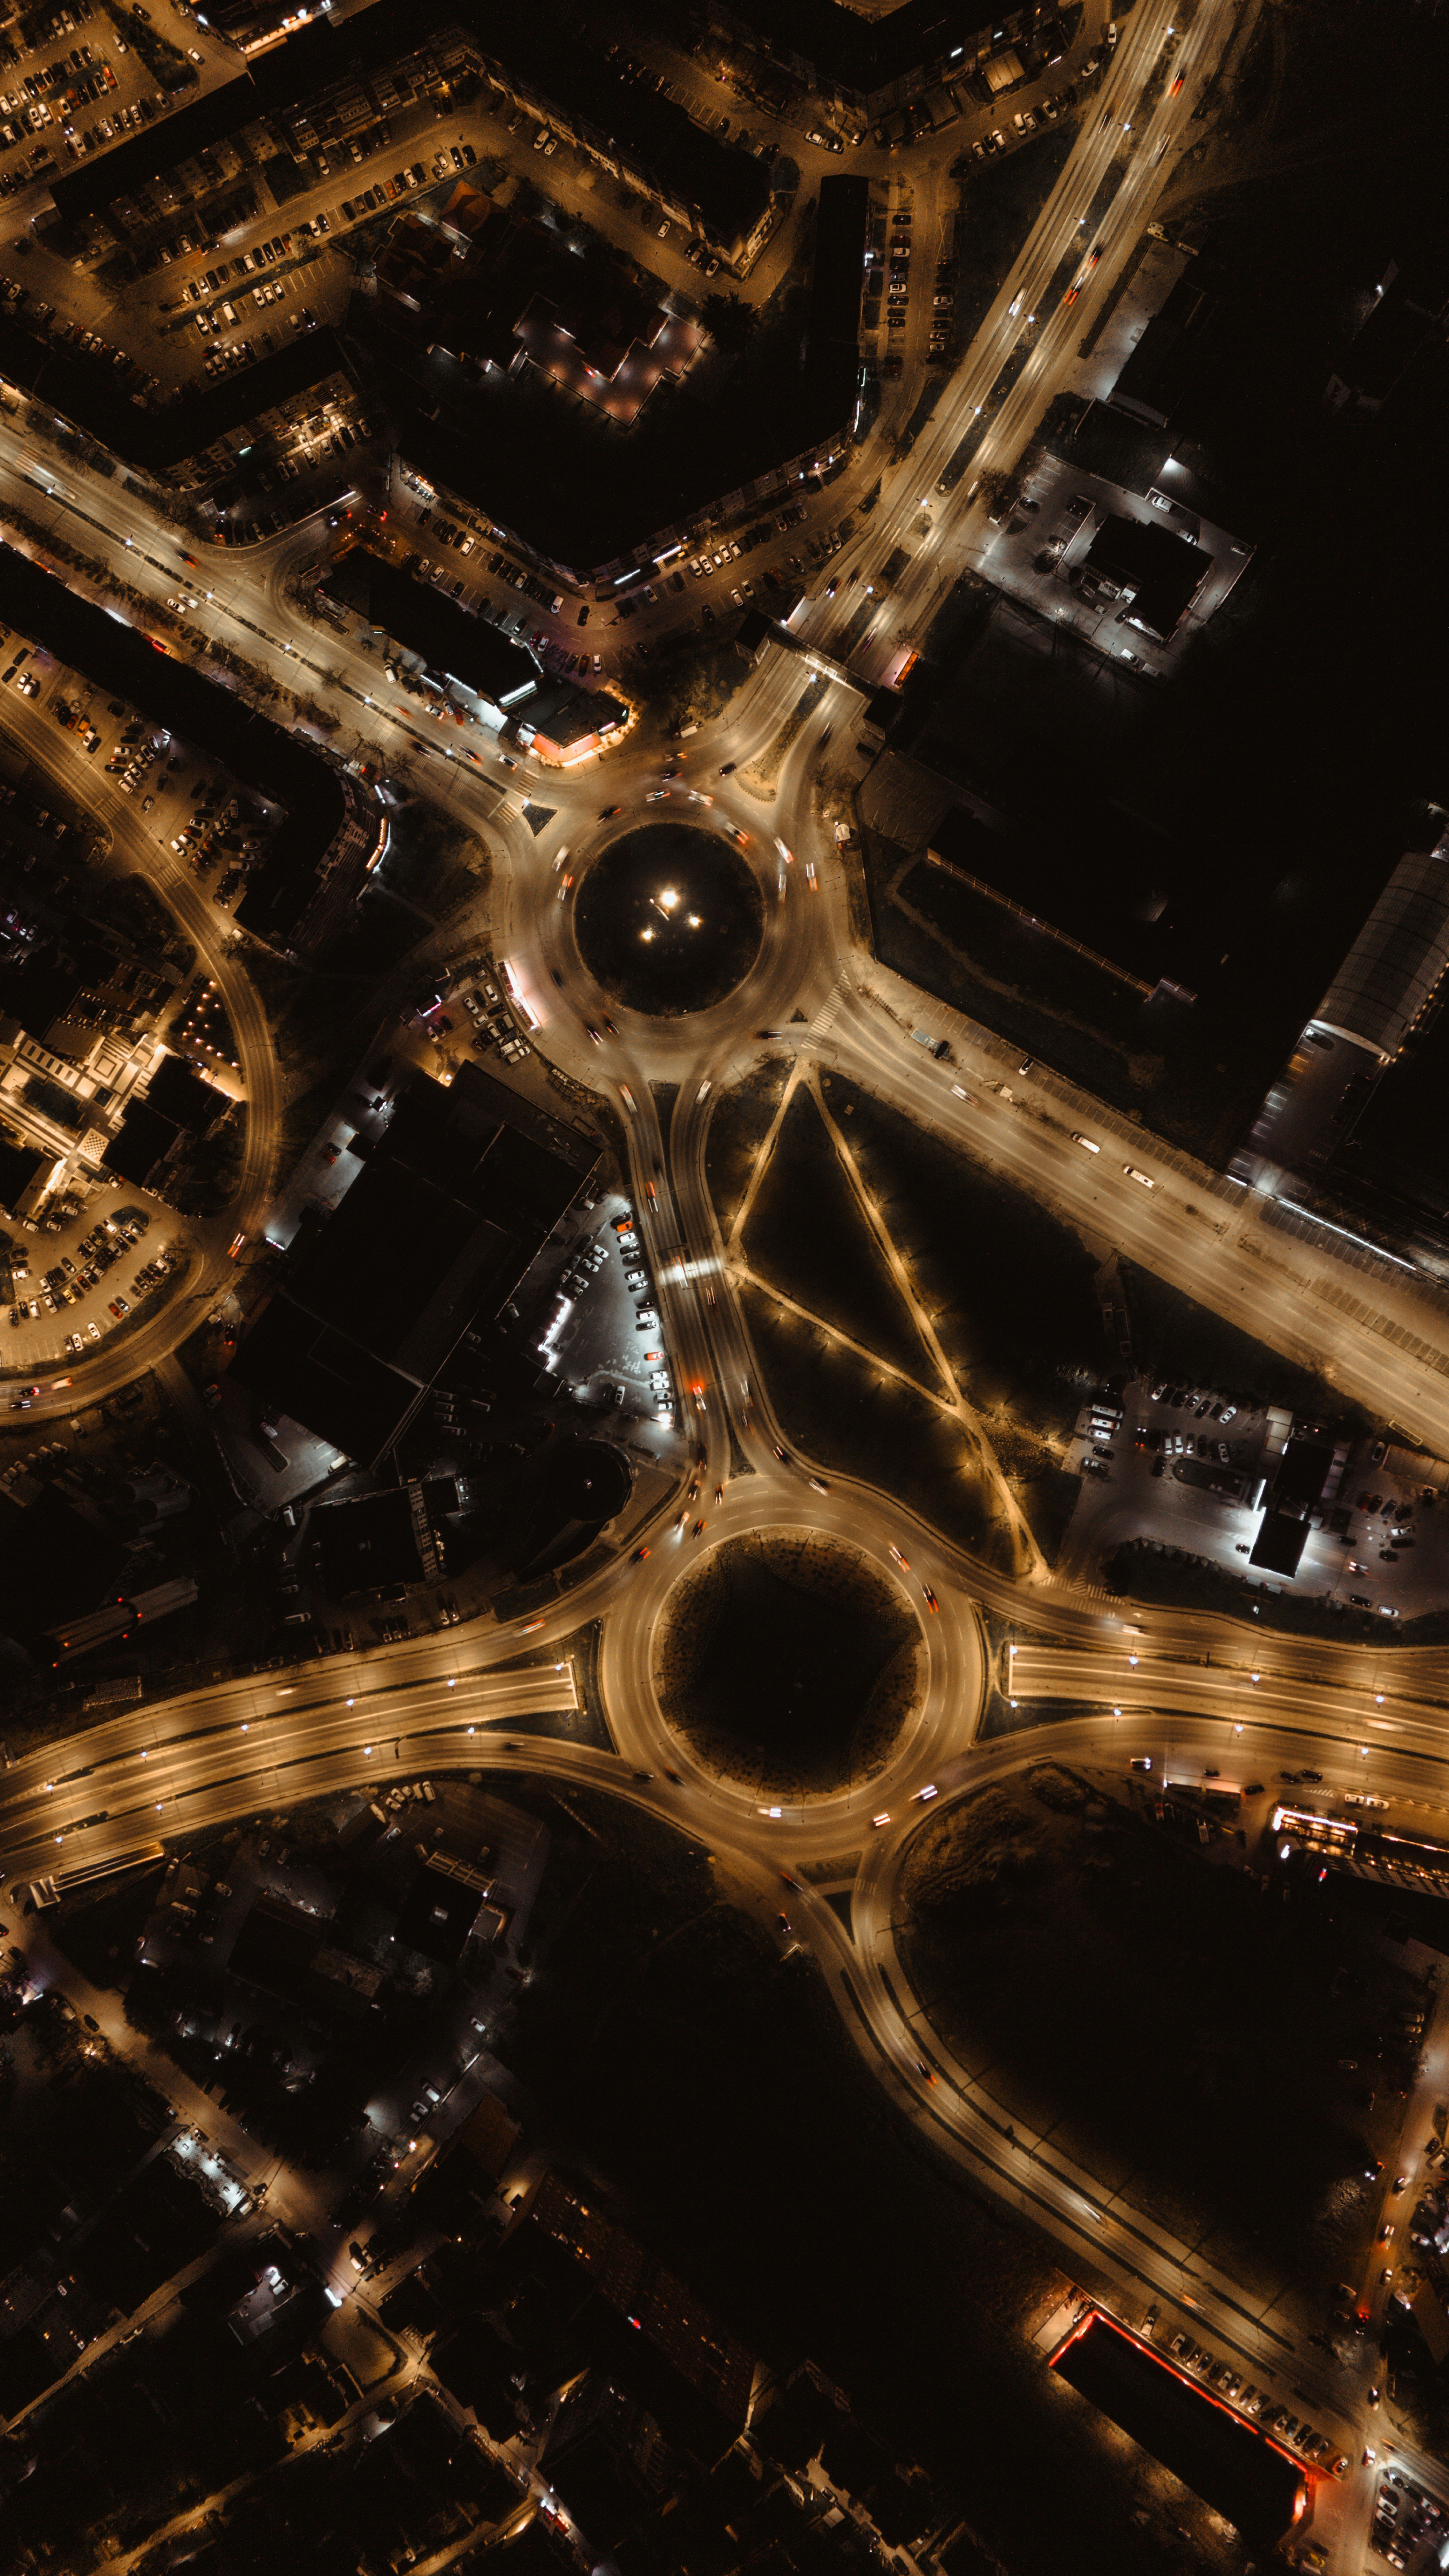
\includegraphics[width=\paperwidth, height=\paperheight]{background2.jpg}
        }
    }
    
    \centering
    \color{white} % Chuyển màu chữ thành màu trắng (hoặc màu tương phản với ảnh nền)
    
    \vspace*{1cm}
    {\large \textbf{BỘ GIÁO DỤC VÀ ĐÀO TẠO}} \\[0.5cm]
    {\large \textbf{TRƯỜNG TRUNG CẤP Y KHOA VIỆT NAM}} \\[3cm]
    
    {\large \textbf{TÀI LIỆU TỔNG HỢP}} \\[0.5cm]
    {\Huge \bfseries KỸ THUẬT THỰC HÀNH \\[0.2cm] VÀ HUYỆT VỊ} \\[4cm]

    \vfill
    
    \begin{flushright}
        \begin{tabular}{ll}
            \textbf{GVHD:} & Trương Văn Chúc \\
            \textbf{SVTH:} & Dương Tiến Mạnh \\
            \textbf{Lớp:} & K12 - Xoa bóp bấm huyệt \\
        \end{tabular}
    \end{flushright}
    
    \vspace{2cm}
    {\large Hà Nội, năm 2026}

\end{titlepage}

% Từ trang sau, ảnh nền sẽ tự động biến mất và màu chữ quay lại mặc định
\newpage 

\nopagebreak % Giữ định dạng liền mạch nếu cần
\section*{Lời cảm ơn}
Để hoàn thiện được bài tiểu luận này một cách tốt nhất,
em xin gửi lời cảm ơn chân thành đến Ban giám hiệu, các phòng ban, khoa
và các thầy cô giảng viên trường trung cấp y khoa Việt Nam và các bạn học viên
đã tận tình dạy dỗ và tạo điều kiện cho em trong quá nghiên cứu và học tập.
Đặc biêt, em muốn gửi lời cảm ơn sâu sắc đến thầy/cô Trương Văn Chúc.
Người đã trực tiếp hướng dẫn em nghiên cứu đề tài này một cách rất nhiệt tình và tận tâm.
Do sự hiểu biết còn hạn chế nên trong bài tiểu luận có thể không tránh khỏi 
còn nhiều thiếu sót. Em mong nhận được sự góp ý của các thầy cô, 
để bài tiểu luận được hoàn thiện tốt hơn. Em xin chân thành cảm ơn các thầy cô!


\tableofcontents
\newpage

\section{Động tác xoa bóp bấm huyệt}

\subsection{Thủ thuật tác động lên da}

\begin{longtblr}[
    caption = {Thủ thuật tác động lên da},
]{
    width = \textwidth,
    colspec = {|X[1,c]|X[1,l]|X[2.5,l]|X[2.5,l]|X[2.5,l]|X[2.5,l]|},
    % hlines,
    rowhead = 1,
}
    \hline
    ID & Thủ thuật & Cơ quan thực hiện & Yêu cầu & Vùng tác động & Quỹ đạo \\ \hline
    1 & \xoa & {%
        1. Gốc bàn tay \newline
        2. Ô mô út \newline
        3. Ngón tay cái
    } & {%
        1. Chậm \newline
        2. Nhẹ
    } & {%
        1. Bụng
    } & {%
        1. Đường tròn
    }
    \\ \hline
    2 & \xat & {%
        1. Gốc bàn tay \newline
        2. Mô ngón út \newline
        3. Ngón tay cái
    } & {%
        1. Nhanh \newline
        2. Có lực
    } & {%      
    } & {%
        1. Lên xuống \newline
        2. Phải sang trái
    }
    \\ \hline
    3 & \miet & {%
        1. Ngón tay cái
    } & {
        1. Chậm \newline
        2. Có lực
    } & {%
        1. Bụng \newline
        2. Đầu
    } & {%
        1. Trên xuống \newline
        2. Dưới lên \newline
        3. Phải sang trái \newline
        4. Trái sang phải
    }
    \\ \hline
    4 & \phanhop & {%
        1. Ngón tay cái \newline
        2. Đầu của ba ngón: 2, 3, 4 \newline
        3. Ô mô út
    } & {%
        1. Kéo đều ra hai bên (phân) \newline
        2. Từ hai bên kéo vào (hợp)
    } & {%
        1. Trán \newline
        2. Đầu \newline
        3. Mặt \newline
        4. Bụng \newline
        5. Lưng \newline
        6. Ngực
    } & {%
        1. Phân hợp ngang \newline
        2. Phân hợp v
    }
    \\ \hline
    5 & \veo & {%
        1. Đầu ngón tay cái và ngón tay trỏ
    } & {%
        1. Kéo da \newline
        2. Da luôn bị cuộn ở giữa các ngón tay
    } & {%
        1. Lưng \newline
        2. Trán
    } & {%
        1. Tịnh tiến
    }
    \\ \hline
    6 & \vo & {%
        1. Bàn tay
    } & {%
        1. Khum bàn tay (lòng bàn tay lõm) \newline
        2. Phát nhẹ tăng dần
    } & {
        1. Vai \newline
        2. Lưng \newline
        3. Tứ chi
    } & {%
        1. Tịnh tiến
    }
    \\ \hline
\end{longtblr}


\subsection{Thủ thuật tác động lên cơ}

\begin{longtblr}[
    caption = {Thủ thuật tác động lên cơ},
]{
    width = \textwidth,
    colspec = {|X[1,c]|X[1,l]|X[2.5,l]|X[2.5,l]|X[2.5,l]|X[2.5,l]|},
    % hlines,
    rowhead = 1,
}
    \hline
    ID & Thủ thuật & Cơ quan thực hiện & Yêu cầu & Vùng tác động & Quỹ đạo
    \\ \hline
    1 & \acday & {%
    1. Mô út \newline
    2. Gốc bàn tay
    } & {%
    1. Khoan thai \newline
    2. Ấn vừa với sức chịu đựng của người bệnh. 
    } & {%
    } & {%
    1. Đường tròn \newline
    }
    \\ \hline
    2 & \dam & {%
    } & {%
    } & {%
    } & {%
    }
    \\ \hline
    3 & \chat & {%
    1. Bàn tay \newline
    2. Cổ tay
    } & {%
    1. Cổ tay mềm dẻo \newline
    2. Tiếng kêu của bàn tay
    } & {%
    1. Cổ gáy \newline
    2. Vai \newline
    3. Lưng \newline
    4. Mông
    } & {%
    }
    \\ \hline
    4 & \lan & {%
    1. Mặt bên ngoài của mô út \newline
    2. Mặt ngoài ngón út
    } & {%
    1. Khéo léo vận động khớp cổ tay \newline
    2. Có lực điệu \newline
    3. Có sức ép nhất định
    } & {%
    1. Lưng \newline
    2. Vai \newline
    3. Mông \newline
    4. Tứ chi \newline
    } & {
    }
    \\ \hline
    5 & \bop & {%
    1. Ngón một và ngón hai \newline
    2. 5 ngón
    } & {%
    1. Kéo vùng cơ của người bệnh. \newline
    2. Vừa phải tránh đau đớn.
    } & {%
    1. Cổ \newline
    2. Gáy \newline
    3. Vai \newline
    4. Nách \newline
    5. Tứ chi
    } & {%
    }
    \\ \hline
    6 & Vờn & {%
    1. Hai bàn tay
    } & {%
    1. Hai bàn tay bao lấy vị trí nhất định. \newline
    2. Da thịt chuyển động theo \newline
    3. Nhẹ nhàng
    } & {%
    } & {%
    1. Ngược chiều \newline
    2. Trên xuống \newline
    3. Dưới lên
    }
    \\ \hline
\end{longtblr}

\subsection{Vận động}
\subsubsection{Vận động khớp cổ}

\begin{longtblr}[
    caption = {Vận động khớp cổ},
]{
    width = \textwidth,
    colspec = {|X[1,c]|X[1,c]|X[1,c]|X[9,l]|},
    % hlines,
    rowhead = 1,
}
    \hline
     STT & Động tác & Số lượt & Ghi chú
     \\ \hline
     1 & Cúi & 3 & {
        \cui
        \newline
        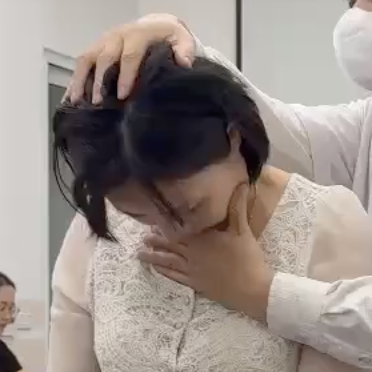
\includegraphics[width=0.48\linewidth]{cui_01.png}
        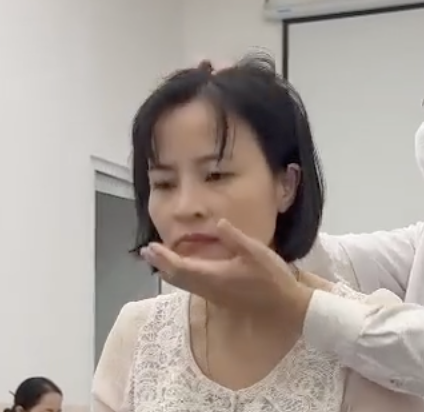
\includegraphics[width=0.48\linewidth]{cui_02.png}
        \newline
        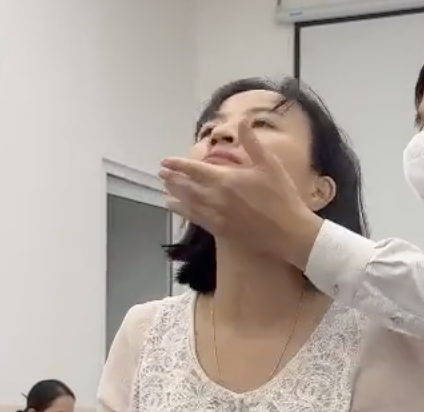
\includegraphics[width=0.48\linewidth]{cui_03.png}
        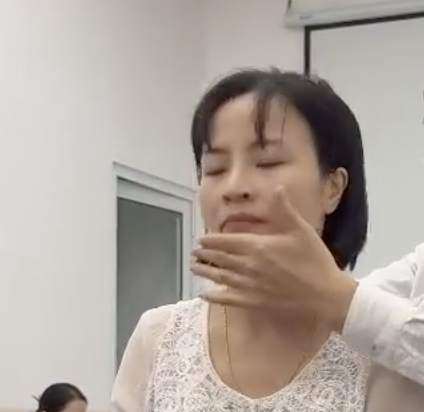
\includegraphics[width=0.48\linewidth]{cui_04.png}
     }
    \\ \hline
    2 & Ngửa & 3 & {
        \ngua (Sau khi đẩy trán thì bỏ tay ra để cổ duỗi thẳng tự nhiên)
        \newline
        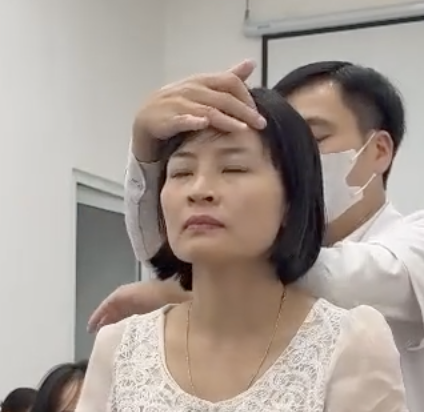
\includegraphics[width=0.48\linewidth]{ngua_01.png}
        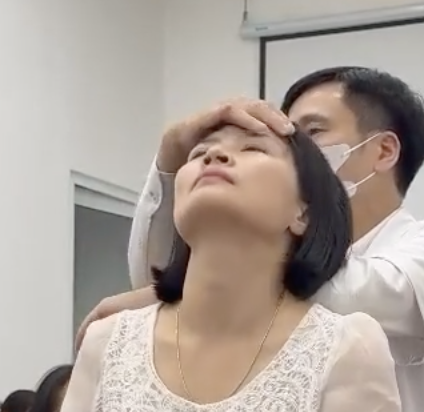
\includegraphics[width=0.48\linewidth]{ngua_02.png}
     }
    \\ \hline
    3 & Nghiêng trái & 3 & {
        \nhiengtrai
        \newline
        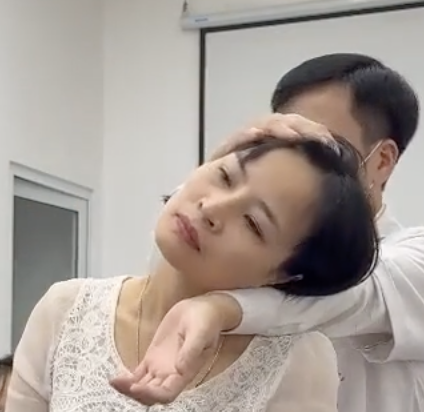
\includegraphics[width=\linewidth]{nghientrai_01.png}
    }
    \\ \hline
    4 & Nghiêng phải & 3 &{
        \nhiengphai
        \newline
        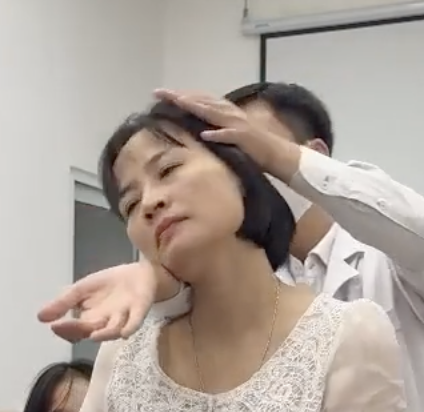
\includegraphics[width=\linewidth]{nghieng_phai_01.png}
    }
    \\ \hline
    4 & Xoay trái & 3 & {
        \xoaytrai: Tới tầm là thôi. Căng tay là dừng 
        \newline
        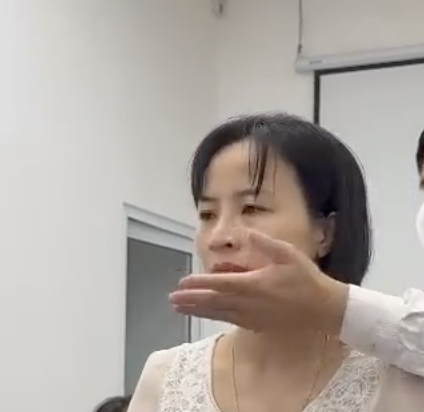
\includegraphics[width=0.48\linewidth]{xoay_trai_01.png}
        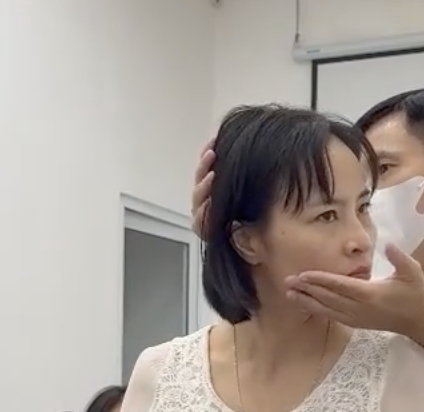
\includegraphics[width=0.48\linewidth]{xoay_trai_02.png}
        \newline
        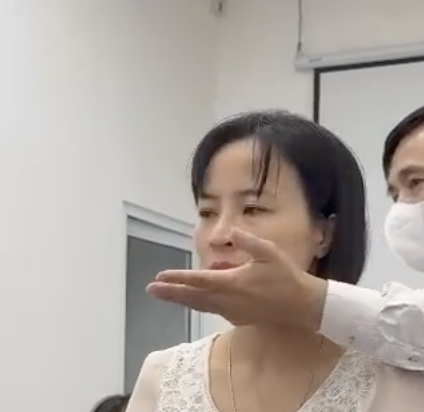
\includegraphics[width=\linewidth]{xoay_trai_03.png}
     }
     \\ \hline
    5 & Xoay phải & 3 & {
        \xoayphai: Tới tầm là thôi. Căng tay là dừng
        \newline
        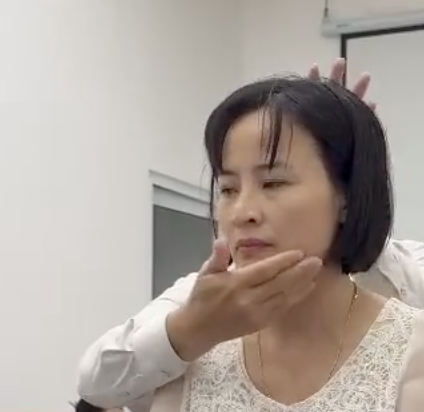
\includegraphics[width=0.48\linewidth]{xoay_phai_01.png}
        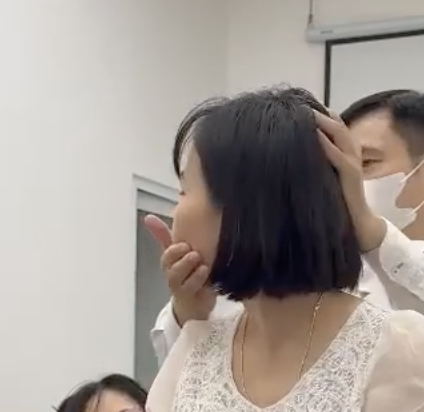
\includegraphics[width=0.48\linewidth]{xoay_phai_02.png}
        \newline
        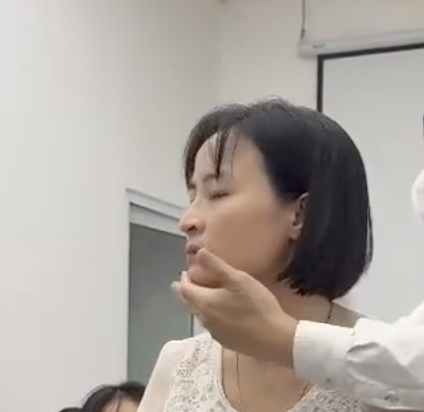
\includegraphics[width=0.48\linewidth]{xoay_phai_03.png}
        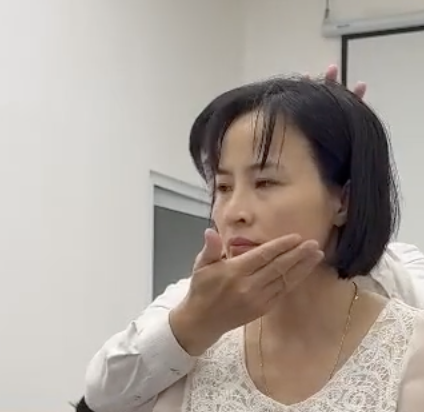
\includegraphics[width=0.48\linewidth]{xoay_phai_04.png}
     }
     \\ \hline
     6 & Xoay hỗn hợp & 3 & {
        \xoayhonhop \newline
        1. Một tay đỡ cằm \newline
        2. Một tay đỡ chẩm \newline
        3. Xoay
        \newline
        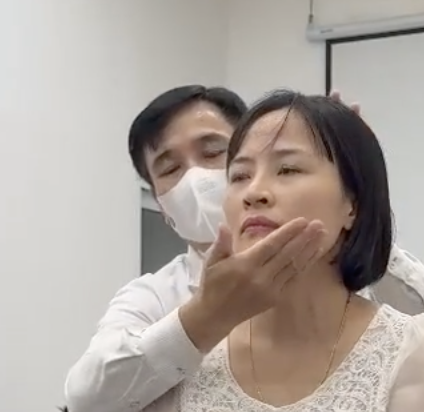
\includegraphics[width=0.48\linewidth]{xoay_hon_hop_01.png}
        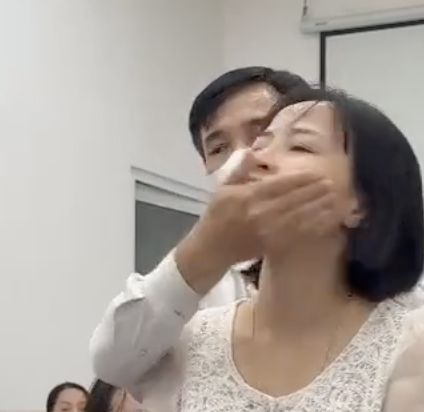
\includegraphics[width=0.48\linewidth]{xoay_hon_hop_02.png}
     }
     \\ \hline
\end{longtblr}

\subsubsection{Vận động khớp tay}

\textbf{Vận động khớp vai}

\begin{longtblr}[
    caption = {Vận động khớp vai},
]{
    width = \textwidth,
    colspec = {|X[1,c]|X[1,c]|X[1,c]|X[9,l]|},
    % hlines,
    rowhead = 1,
}
    \hline
    STT & Tên & Số lần & Ghi chú
    \\ \hline
    1 & Xoay vòng nhỏ & & {%
        \hypertarget{target:xoay_vong_nho}{\textbf{Xoay vòng nhỏ:}}

        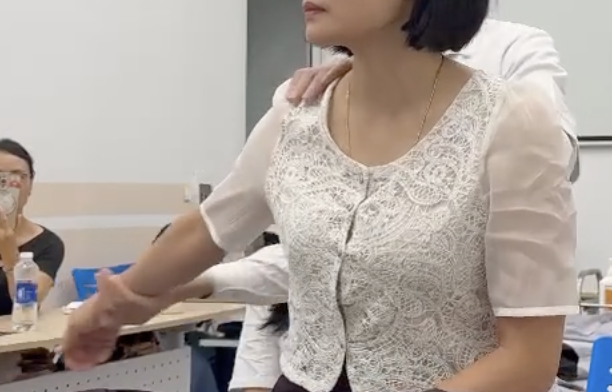
\includegraphics[width=0.48\linewidth]{van_dong_kho_vai_02.png}
        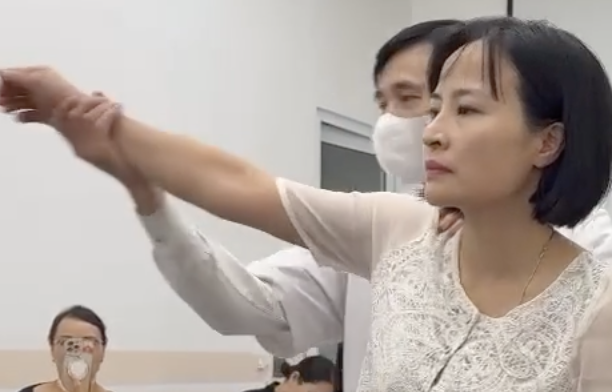
\includegraphics[width=0.48\linewidth]{van_dong_khop_vai_02.png}
    }
    \\ \hline
    2 & Xoay vòng lớn & & {%
        \hypertarget{target:xoay_vong_lon}{\textbf{Xoay vòng lớn:}} bao gồm xoay xuôi và xoay ngược

        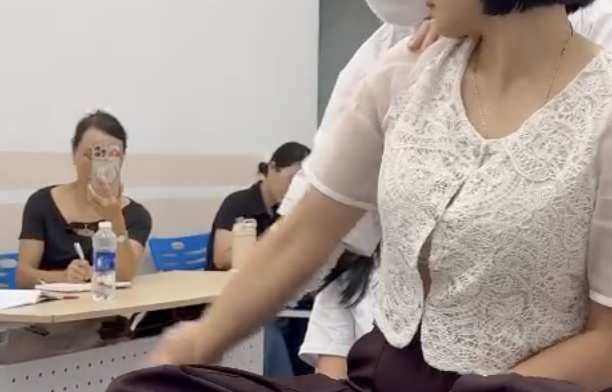
\includegraphics[width=0.48\linewidth]{xoay_vong_lon_01.png}
        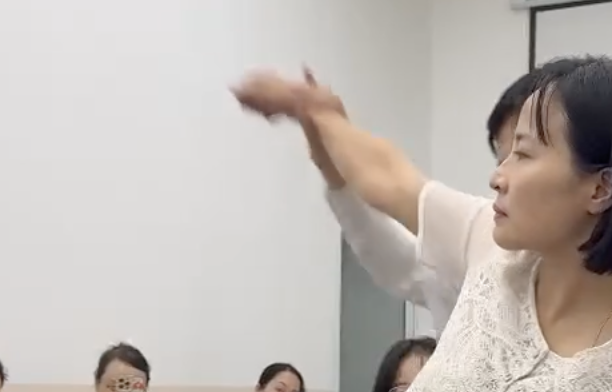
\includegraphics[width=0.48\linewidth]{xoay_khop_vai_02.png}
    }
    \\ \hline
    3 & Xoay mở khớp vai & & {%
        \hypertarget{target:xoay_mo_khop_vai}{\textbf{Xoay mở khớp vai:}} Lựa tới tầm căng cơ

        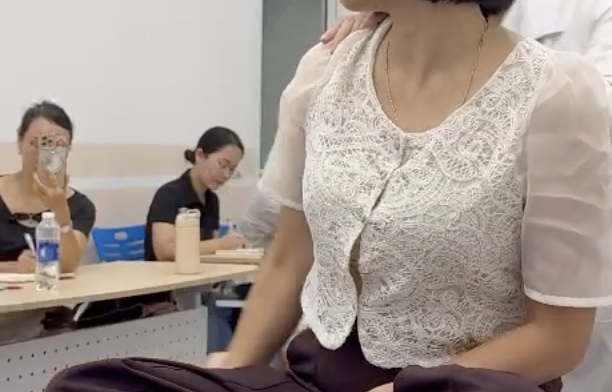
\includegraphics[width=0.48\linewidth]{xoay_mo_khop_vai_0.png}
        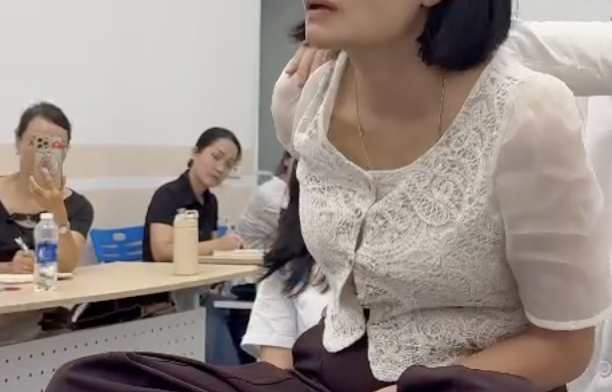
\includegraphics[width=0.48\linewidth]{xoay_mo_khop_vai_02.png}
    }
    \\ \hline
    4 & Mở khớp vai & & {%
        \hypertarget{target:mo_khop_vai}{\textbf{Mở khớp vai:}}

        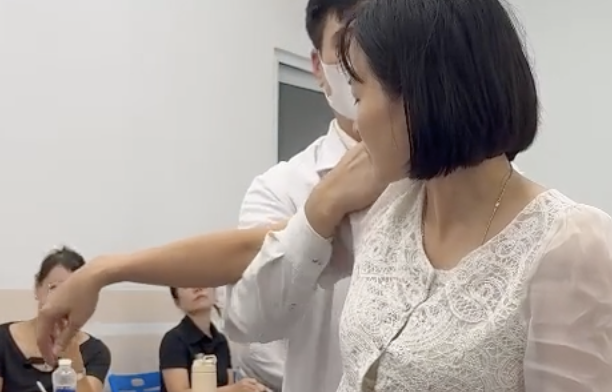
\includegraphics[width=0.48\linewidth]{mo_khp_vai.png}
        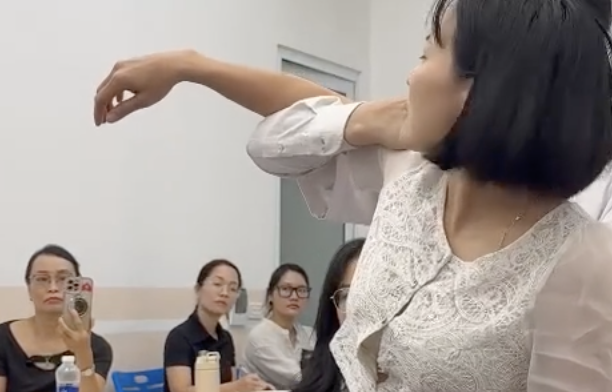
\includegraphics[width=0.48\linewidth]{mo_khop_vai_02.png}
    }
    \\ \hline
\end{longtblr}

\textbf{Vận động khuỷu tay}
\begin{longtblr}[
    caption = {Vận động khuỷu tay},
]{
    width = \textwidth,
    colspec = {|X[1,c]|X[1,c]|X[1,c]|X[9,l]|},
    % hlines,
    rowhead = 1,
}
    \hline
    STT & Tên & Số lần & Ghi chú
    \\ \hline
    1 & Gấp duỗi & 1 & {
        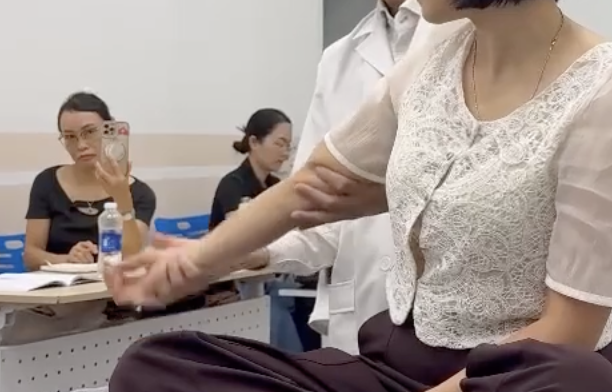
\includegraphics[width=0.48\linewidth]{khop_vai_01.png}
        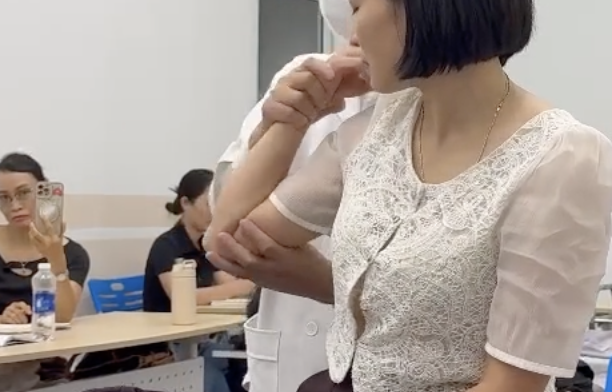
\includegraphics[width=0.48\linewidth]{khop_vai_02.png}
    }
    \\ \hline
    2 & Sấp ngửa & 1 & {
        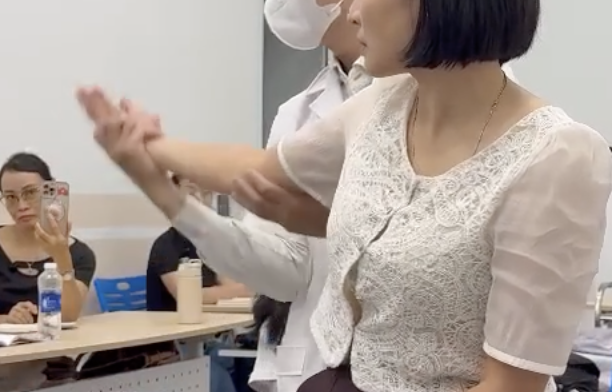
\includegraphics[width=0.48\linewidth]{sap_ngua_01.png}
        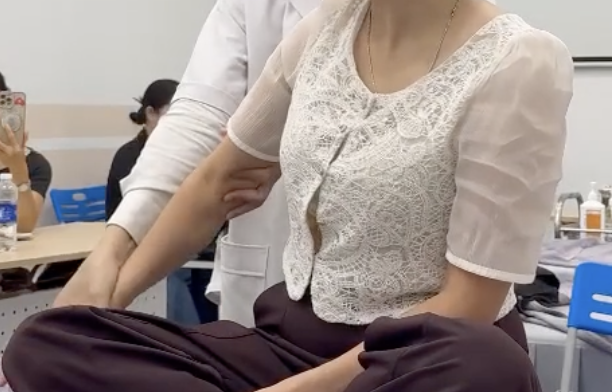
\includegraphics[width=0.48\linewidth]{sap_ngua_02.png}
    }
    \\ \hline
\end{longtblr}


\textbf{Vận động cổ tay}
\begin{longtblr}[
    caption = {Vận động cổ tay},
]{
    width = \textwidth,
    colspec = {|X[1,c]|X[1,c]|X[1,c]|X[9,l]|},
    % hlines,
    rowhead = 1,
}
    \hline
    STT & Tên & Số lần & Ghi chú
    \\ \hline
    1 & Xoay & & {
        Xoay ngược, xoay xuôi
        \newline
        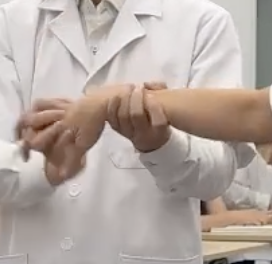
\includegraphics[width=0.48\linewidth]{xoay_co_tay_01.png}
        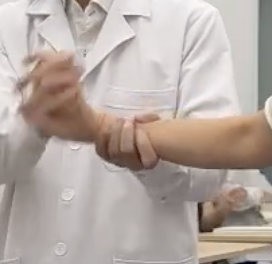
\includegraphics[width=0.48\linewidth]{xoay_co_tay_02.png}
    }
    \\ \hline
    2 & Gấp duỗi & & {
        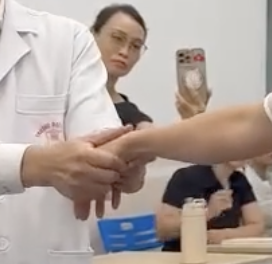
\includegraphics[width=0.48\linewidth]{gap_duoi_01.png}
        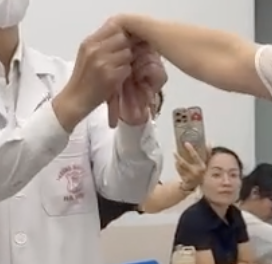
\includegraphics[width=0.48\linewidth]{gap_duoi_02.png}
        \newline
        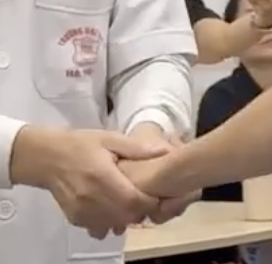
\includegraphics[width=0.48\linewidth]{gap_duoi_03.png}
        \newline
        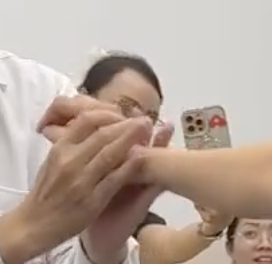
\includegraphics[width=0.48\linewidth]{duoi_01.png}
        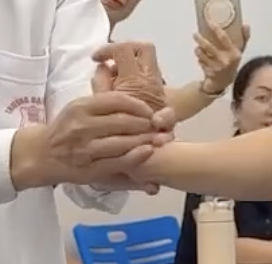
\includegraphics[width=0.48\linewidth]{duoi_02.png}
    }
    \\ \hline
\end{longtblr}

\textbf{Vận động ngón tay}
\begin{longtblr}[
    caption = {Vận đống ngón tay},
]{
    width = \textwidth,
    colspec = {|X[1,c]|X[1,c]|X[1,c]|X[9,l]|},
    % hlines,
    rowhead = 1,
}
    \hline
    STT & Tên & Số lần & Ghi chú
    \\ \hline
    1 & Vê & 5 & {
        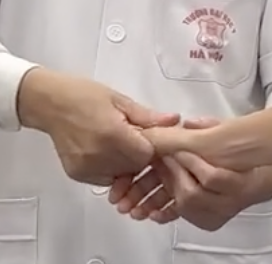
\includegraphics[width=\linewidth]{ve_ngon_tay_01.png}
    }
    \\ \hline
    2 & Vuốt & 5 & {
        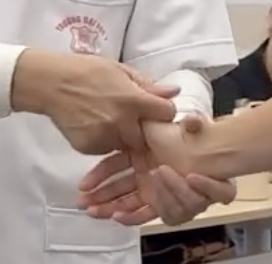
\includegraphics[width=\linewidth]{vuot_ngon_tay_01.png}
    }
    \\ \hline
\end{longtblr}


\textbf{Rung tay}
\begin{longtblr}[
    caption = {Rung tay},
]{
    width = \textwidth,
    colspec = {|X[1,c]|X[1,c]|X[1,c]|X[9,l]|},
    % hlines,
    rowhead = 1,
}
    \hline
    STT & Tên & Số lần & Ghi chú
    \\ \hline
    1 & Rung tay &  & {
    1. Bệnh nhân hơi nghiêng đối diện \newline
    2. Trước sau \newline
    3. Trên dưới \newline
    4. Kéo dãn
    \newline
    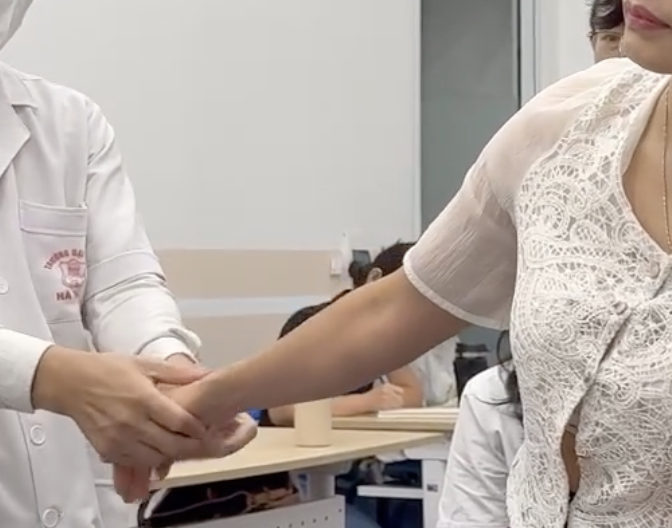
\includegraphics[width=0.48\linewidth]{rung_tay_01.png}
    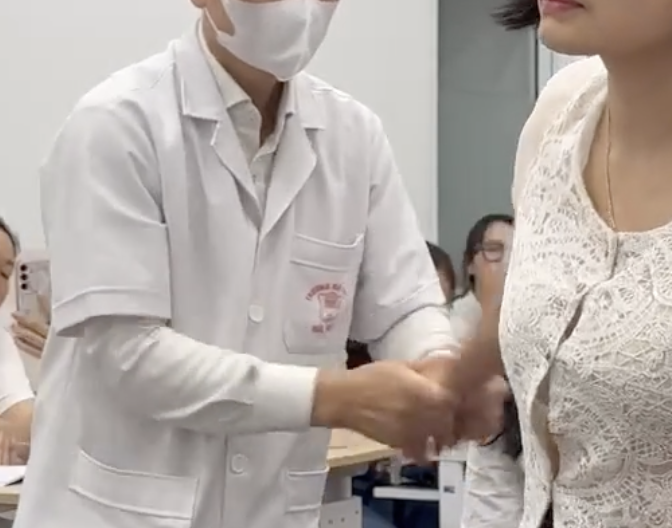
\includegraphics[width=0.48\linewidth]{rung_tay_02.png}
    \newline
    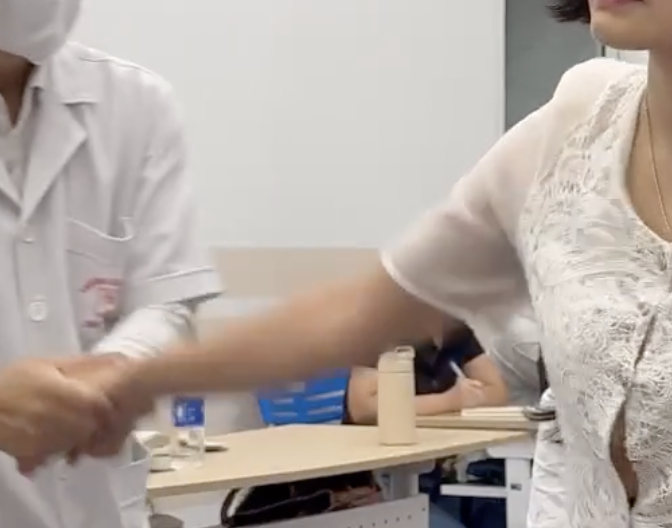
\includegraphics[width=0.48\linewidth]{rung_tay_03.png}
    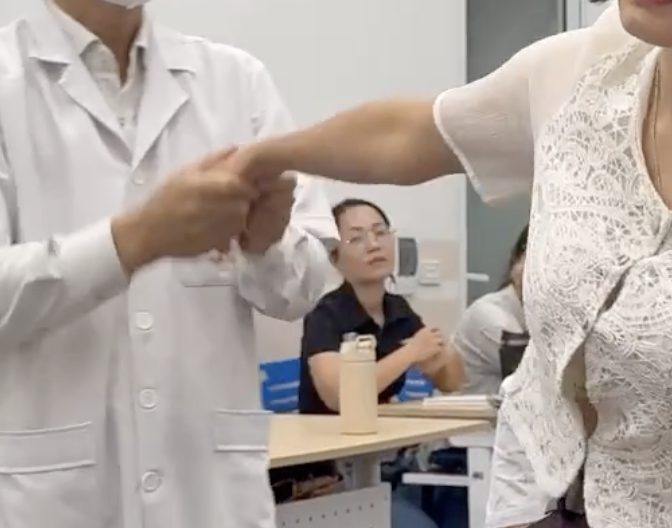
\includegraphics[width=0.48\linewidth]{rung_tay_04.png}
    \newline
    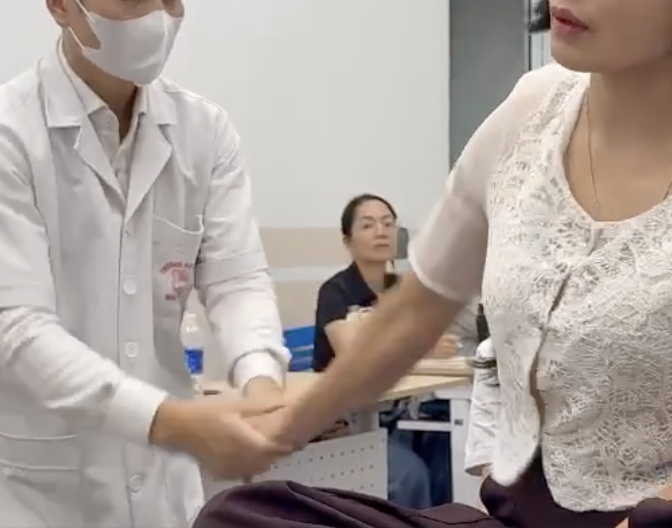
\includegraphics[width=\linewidth]{rung_tay_05.png}
    }
    \\ \hline
\end{longtblr}


\subsubsection{Vận động khớp chân}
\textbf{TƯ THẾ NẰM NGHIÊNG}

\begin{longtblr}[
    caption = {Vận động khớp tư thế nằm nghiêng},
]{
    width = \textwidth,
    colspec = {|X[1,c]|X[1,l]|X[2,l]|X[1,c]|X[7,l]|},
    % hlines,
    rowhead = 1,
}
    \hline
    STT & Tên & Vùng tác động & Số lần & Ghi chú
    \\ \hline
    1 & Vận động & Cột sống và thắt lưng cùng &  & {
        Vận động khớp cùng chậu
    
        Chi bị bệnh ở trên, thầy thuốc đứng sau người bệnh, 1 tay đặt ở khớp cùng chậu, một tay kéo giãn chi dưới và gấp nhanh chi dưới vào bụng, tay kia vẫn giữ chặt khớp cùng chậu.

        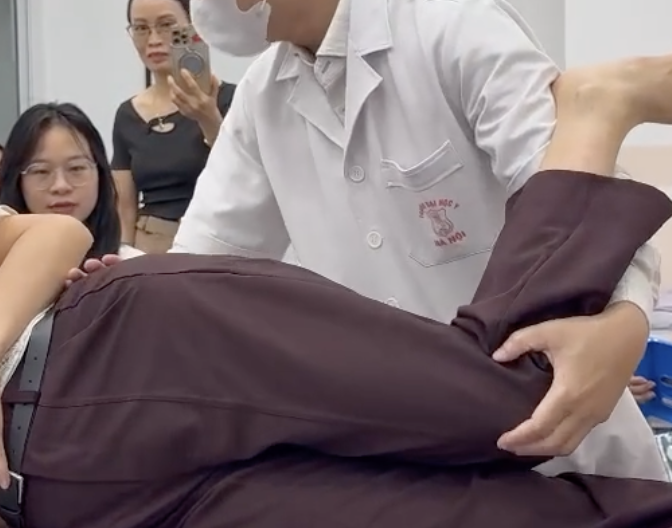
\includegraphics[width=\linewidth]{day_dau_goi_tu_the_nam_nghieng_01.png}
        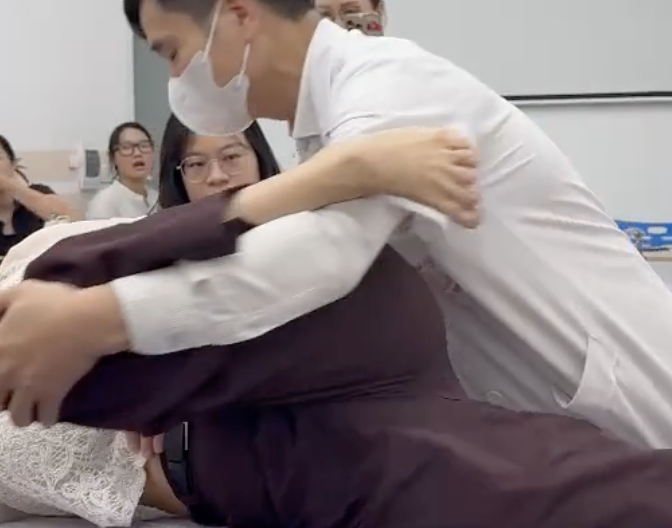
\includegraphics[width=\linewidth]{day_dau_goi_tu_the_nam_nghieng_02.png}

        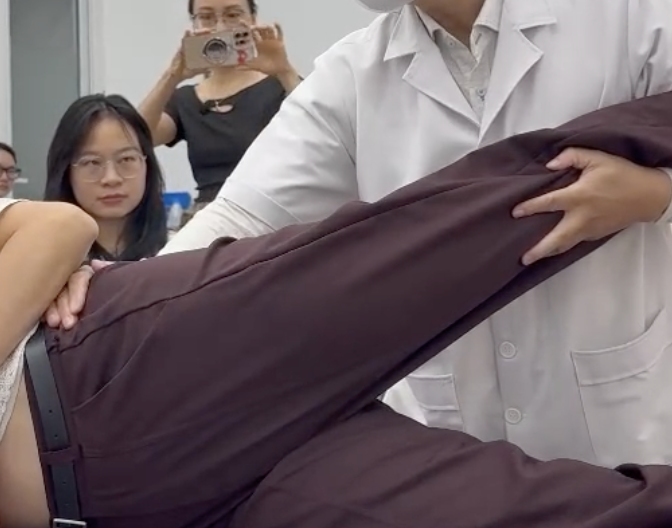
\includegraphics[width=\linewidth]{day_dau_goi_tu_the_nam_nghieng_03.png}
    }
    \\ \hline
    2 & Vận động & Cột sống và thắt lưng cùng & & {
        Vặn cột sống lưng
    
        Người bệnh nằm nghiêng, chân trên co, đầu gối để xuống giường, chân dưới duỗi, tay trên để ra sau lưng, tay dưới để tự nhiên. Thầy thuốc cùng 1 lúc 1 tay đẩy mông ra trước, 1 tay đẩy vai ra sau. Có thể nghe thấy tiếng kêu.   

        Nằm ngược lại và thực hiện tương tự.

        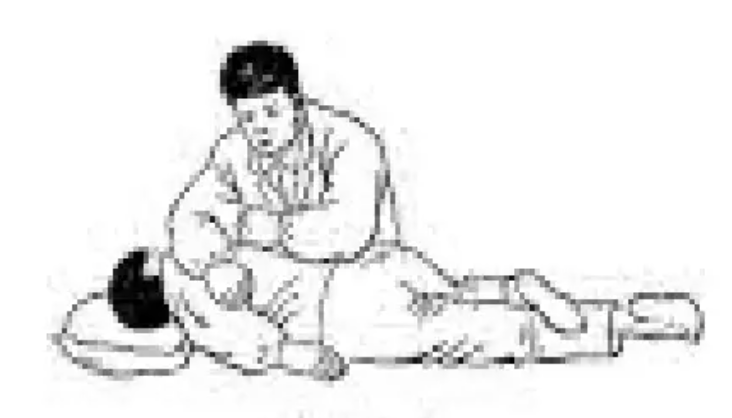
\includegraphics[width=3cm]{van_lung.png}
    }
    \\ \hline
\end{longtblr}


\textbf{TƯ THẾ NẰM NGỬA}

\begin{longtblr}[
    caption = {Vận động khớp tư thế nằm ngửa},
]{
    width = \textwidth,
    colspec = {|X[1,c]|X[1,l]|X[2,l]|X[1,c]|X[7,l]|},
    % hlines,
    rowhead = 1,
}
    \hline
    STT & Tên & Vùng tác động & Số lần & Ghi chú
    \\ \hline
    1 & Vận động & Khớp háng &  & {
        Mở khớp háng

        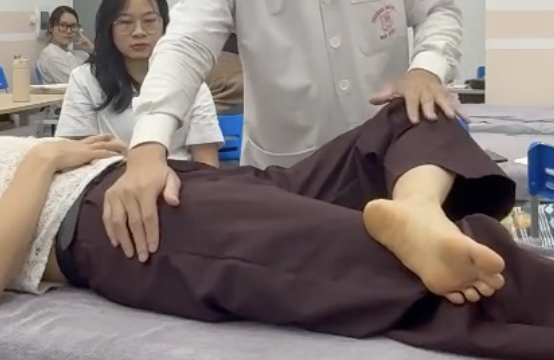
\includegraphics[width=\linewidth]{mo_khop_hang_01.png}
    }
    \\ \hline
    2 & Vận động & Khớp háng  & & {
        \hypertarget{target:van_dong_khop_hang_tu_the_nam_ngua}{\textbf{Vận động khớp háng tư thế nằm ngửa:}}

        Đẩy đầu gối
        
        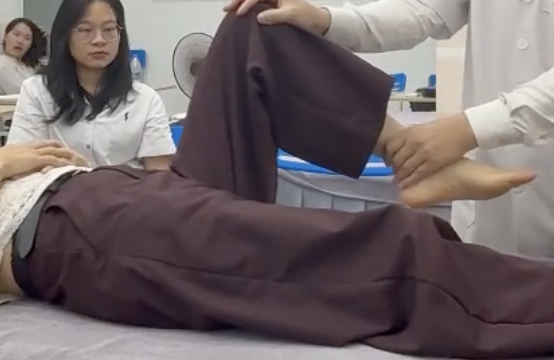
\includegraphics[width=\linewidth]{day_dau_goi_01.png}
        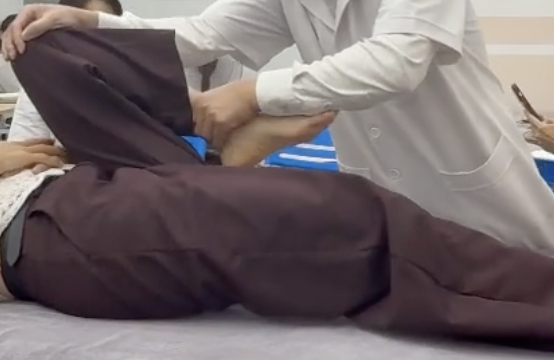
\includegraphics[width=\linewidth]{day_dau_goi_02.png}
    }
    \\ \hline
    3 & Vận động & Cột sống và khớp thắt lưng cùng & & {
        Vận động khớp cùng chậu

        \textbf{Không làm cho thoát vị đĩa đệm}
        
        Co gập chi dưới vào bụng, thầy thuốc một tay giữ chân, một tay đẩy đầu gối người bệnh sang bên phải sang bên trái 2-3 lần.

        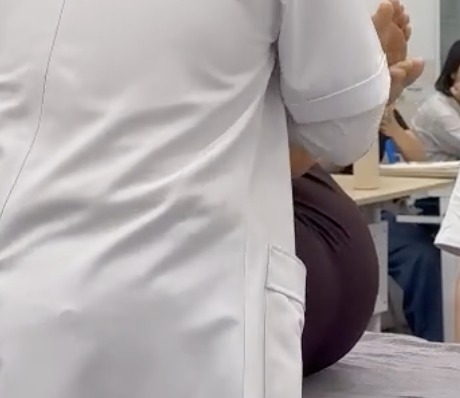
\includegraphics[width=\linewidth]{van_dong_that_lung_cung_01.png}
    }
    \\ \hline
    4 & Vận động & Cột sống và khớp thắt lưng cùng & & {
        Vận động khớp thắt lưng cùng

        Người bệnh nằm ngửa, co gập 2 chi dưới vào bụng, thầy thuốc 1 tay giữ gối, 1 tay để vào vùng cùng cụt làm cho người cong lại, rồi thả ra. 2-3 lần.

        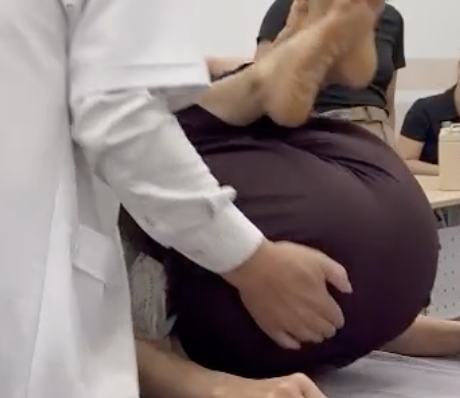
\includegraphics[width=\linewidth]{van_dong_khop_that_lung_cung_01.png}
    }
    \\ \hline
    5 & Vận động & Khớp đầu gối & & {
        Đẩy đầu gối
        \hypertarget{target:day_dau_goi}{\textbf{Đẩy đầu gối:}}

        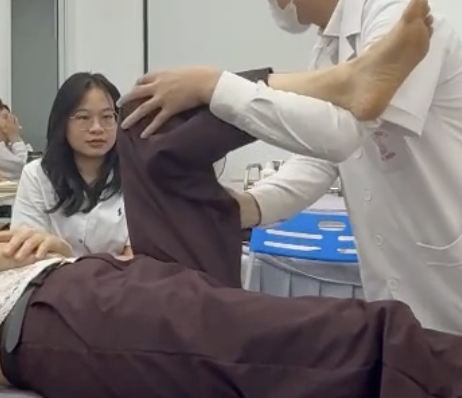
\includegraphics[width=\linewidth]{van_dong_khop_goi_01.png}
        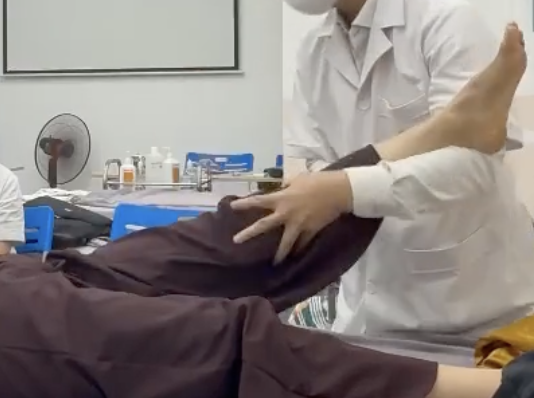
\includegraphics[width=\linewidth]{van_dong_khop_goi_02.png}
    }
    \\ \hline
    6 & Vận động & Khớp cổ chân & & {
        \hypertarget{target:xoay_co_chan}{\textbf{Xoay cổ chân:}}
    }
    \\ \hline
    7 & Vận động & Khớp cổ chân & & {
        \hypertarget{target:gap_duoi_co_chan}{\textbf{Gấp duỗi cổ chân:}}
    }
    \\ \hline
    8 & Vận động & Khớp cổ chân & & {
        \hypertarget{target:nghieng_co_chan}{\textbf{Nghiêng cổ chân:}}
    }
    \\ \hline
    9 & Vận động & Khớp ngón chân & & {
        \hypertarget{target:ve_ngon_chan}{\textbf{Vê ngón chân:}}
    }
    \\ \hline
    10 & Vận động & Khớp ngón chân & & {
        \hypertarget{target:vuot_ngon_chan}{\textbf{Vuốt ngón chân:}}
    }
    \\ \hline
\end{longtblr}

\textbf{TƯ THẾ NẰM SÂP}

\begin{longtblr}[
    caption = {Vận động khớp tư thế nằm sấp},
]{
    width = \textwidth,
    colspec = {|X[1,c]|X[1,l]|X[1,l]|X[1,c]|X[8,l]|},
    % hlines,
    rowhead = 1,
}
    \hline
    STT & Tên & Vùng tác động & Số lần & Ghi chú
    \\ \hline
    1 & Vận động &Cột sống và thắt lưng cùng (dưới) & 2-3  & {
        \noindent \textbf{Không dùng cho bệnh nhân bị thoát vị đĩa đệm.}

        Người bệnh nằm sấp, thầy thuốc 1 tay ấn lưng bệnh nhân,
         một tay nhấc 2 chân bn lên cao.

        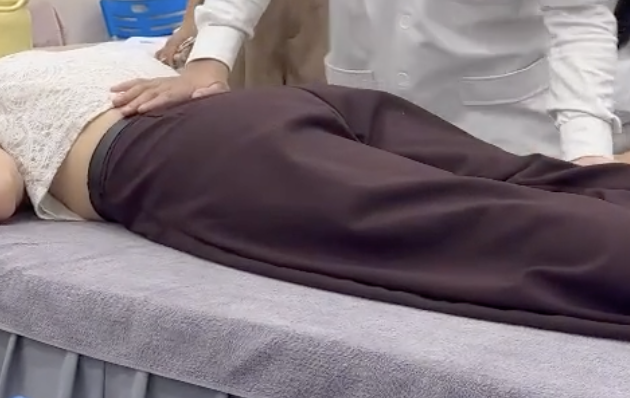
\includegraphics[width=\linewidth]{uon_lung_01.png}
        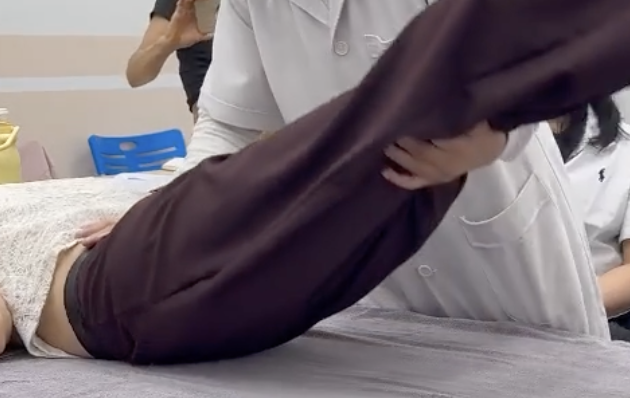
\includegraphics[width=\linewidth]{uon_lung_02.png}
    }
    \\ \hline
    2 & Vận động & Cột sống và thắt lưng cùng (trên) & 2-3 & {
        \noindent \textbf{Không dùng cho bệnh nhân bị thoát vị đĩa đệm.}

        Hai tay bệnh nhân duỗi thẳng lên đỉnh đầu.
        Người trị liệu một tay để ở giữa hai vai bệnh nhân,
        cánh tay dưới của cánh tay còn lại đỡ lấy phần trên khuỷu tay của bệnh nhân.
        Sau đó tay đẩy tay nâng thực hiện động tác.
    }
    \\ \hline
    1 & Vận động & Khớp háng & 3-5 & {
        \hypertarget{target:van_dong_khop_hang_tu_the_nam_sap}{\textbf{Vận động khớp háng tư thế nằm sấp:}}
        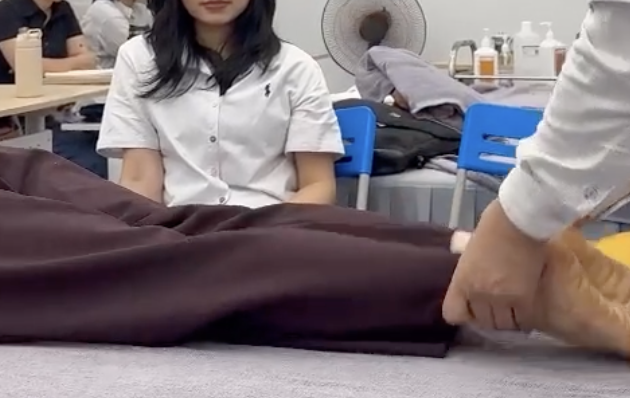
\includegraphics[width=\linewidth]{van_dong_khop_hang_tu_the_nam_sap_01.png}
        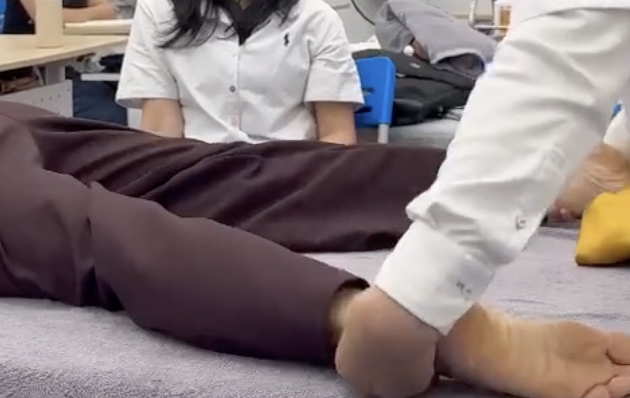
\includegraphics[width=\linewidth]{van_dong_khop_hang_tu_the_nam_sap_02.png}
    }
    \\ \hline
    1 & Vận động & Khớp gối & 3-5 & {
        \hypertarget{target:van_dong_khop_goi_tu_the_nam_sap}{\textbf{Vận động khớp gối tư thế nằm sấp:}}
        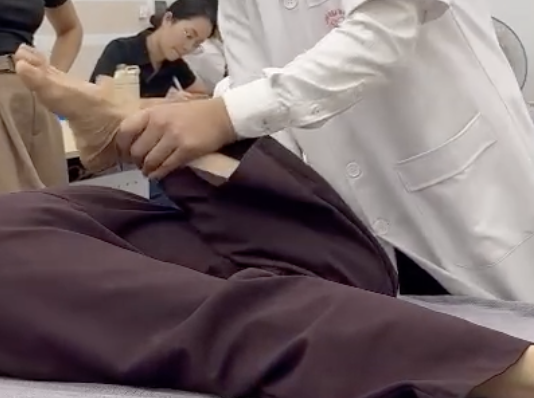
\includegraphics[width=\linewidth]{van_dong_khop_goi_tu_the_nam_sap_01.png}
        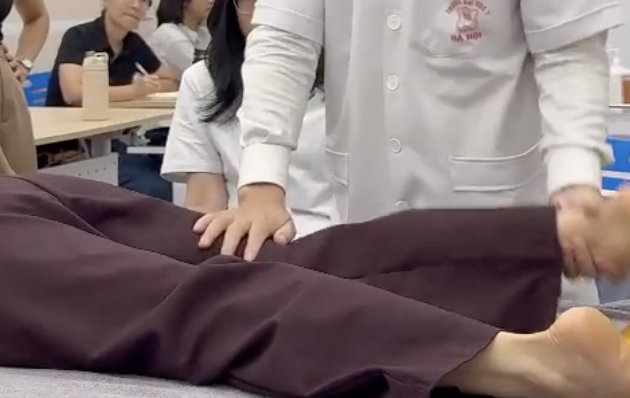
\includegraphics[width=\linewidth]{van_dong_khop_dau_goi_tu_the_nam_sap_02.png}
    }
    \\ \hline
\end{longtblr}

\section{Thủ thuật}

\subsection{Thủ thuật vùng đầu}

\begin{longtblr}[
    caption = {Thủ thuật xoa bóp vùng đầu},
]{
    width = \textwidth,
    colspec = {| X[1,c] |X[1, c]|X[2, c]|X[1, c]|X[7, l]|},
    % hlines,
    hspan = minimal,
    rowhead = 1,
}
    \hline
    ID & Động tác & Vùng tác động & Số lần & Huyệt
    \\ \hline
    1 & Chải & Đầu & 3-5 & {
        Trước ra sau. Trên sang hai bên
    }
    \\ \hline
    2 & Miết & Trán & 3-5 & {
        Miết từ ấn đường ra chân mày.
        Theo hình dẻ quạt ra hai bên.
    }
    \\ \hline
    3 & Miết & Huyệt & 3-5 & {
        Ấn Đường, Thái Dương, Đầu Duy, Xuất Cốc, Phong Trì
    }
    \\ & & & & {
        Ấn Đường
        \anduong
    }
    \\ & & & & {
        Thái Dương
        \thaiduong
    } 
    \\ & & & & {
        Đầu Duy
        \dauduy
    } 
    \\ & & & & {
        Xuất Cốc
        \xuatcoc
    } 
    \\ & & & & {
        Phong trì
        \phongtri
    }
    \\ \hline
    4 & Phân hợp & Trán & 3-5 & {
        Phân hợp vùng trán, từ ấn đường ra chân mày, phân hợp hết trán, sử dụng ngón tay cái để tiến hành phân hợp.
    }
    \\ \hline
    5 & Véo & Véo từ đầu chân mày đến cuối chân mày & 3-5 & {
        Dùng để xoá nhăn
    }
    \\ & & & & {
        Ấn Đường
        \anduong
    }
    \\ & & & & {
        Thái Dương
        \thaiduong
    }
    \\ \hline
    6 & Vỗ & Đầu, trán & 3-5 & {Vỗ vùng tiếp giáp đầu và trán}
    \\ \hline
    7 & Day & Hốc mắt & 3-5 & {
        Dùng 3 đầu ngón tay giữa.
        Để vô lông mày, kéo ngược lên trán và day.
    }
    \\ \hline
    8 & Day & Đầu, trán & 3-5 & {
        Dùng đầu ngón tay
    }
    \\ \hline
    9 & Chặt & Trán & 3-5 & {
        Chặt xoè vùng đầu trán.
    }
    \\ \hline
    10 & Bóp & Đầu & 3-5 & {
    }
    \\ \hline
    11 & Bấm/Day & Huyệt Ấn Đường & 1 (1 huyệt 1 phút) & {
        Ấn Đường

        \anduong
    }
    \\ \hline
    12 & Bấm/Day & Huyệt Dương Bạch & 1 (1 huyệt 1 phút) & {
        Dương Bạch

        \duongbach
    }
    \\ \hline
    12 & Bấm/Day & Huyệt Đầu Duy & 1 (1 huyệt 1 phút) & {
        Đầu Duy

        \dauduy
    }
    \\ \hline
    13 & Bấm/Day & Huyệt Thái Dương & 1 (1 huyệt 1 phút) & {
        Thái Dương

        \thaiduong
    }
    \\ \hline
    14 & Bấm/Day & Huyệt Hàm Yến & 1 (1 huyệt 1 phút) & {
        Hàm Yên

        \hamyen
    }
    \\ \hline
    15 & Bấm/Day & Huyệt Bách Hội & 1 (1 huyệt 1 phút) & {
        Bách Hội

        \bachhoi
    }
    \\ \hline
    16 & Bấm/Day & Huyệt Tứ Thần Thông & 1 (1 huyệt 1 phút) & {
        Tứ Thần Thông

        \tuthanthong
    }
    \\ \hline
    17 & Bấm/Day & Huyệt Phong Phủ & 1 (1 huyệt 1 phút) & {
        Phong Phủ

        \phongphu
    }
    \\ \hline
    18 & Bấm/Day & Huyệt Thiên Trụ & 1 (1 huyệt 1 phút) & {
        Thiên Trụ

        \thientru
    }
    \\ \hline
    19 & Bấm/Day & Huyệt Phong Trì & 1 (1 huyệt 1 phút) & {
        Phong Trì

        \phongtri
    }
    \\ \hline
\end{longtblr}

\subsection{Thủ thuật vùng vai}

\begin{longtblr}[
    caption = {Thủ thuật xoa bóp vùng vai},
]{
    width = \textwidth,
    colspec = {| X[1,c] |X[1, c]|X[2, c]|X[1, c]|X[7, l]|},
    % hlines,
    rowhead = 1,
}
    \hline
    ID & Động tác & Vùng tác động & Số lần & Huyệt
    \\ \hline
    1 & Xoa & Vai & 3-5 & {}
    \\ \hline
    2 & Xát & Vai & 3-5 & {}
    \\ \hline
    3 & Miết & Vai & 3-5 & {
        Miết ngược từ huyệt cảnh can lên đầu. \newline
        Dưới huyệt cảnh can thì miết xuôi.
    }
    \\ \hline
    4 & Phân hợp & Vai, Cổ & 3-5 & {
        Gáy dùng ngón cái. \newline
        Vai dùng đốt ngón út.
    }
    \\ \hline
    5 & Vỗ & Vai & 3-5 {}
    \\ \hline
    6 & Day & Cổ, Vai & 3-5 & {
        Day cơ thang và cơ ức đòn trũng.
        \newline.
        Day cơ vai
    }
    \\ \hline
    7 & Đấm chặt & Vai & 3-5 & {

    }
    \\ \hline
    8 & Lăn & Cổ vai & 3-5 & {
        Lăn dọc theo đốt sống cách 0.5
        \newline
        Lăn từ trên lăn xuống.
        \newline
        Lăn vai
    }
    \\ \hline
    9 & Bóp & Cổ vai & 3-5 & {
        Bóp gáy chú ý bóp từ xương chũng quay lên dùng một bàn tay.
        \newline
        Vai, lưng thì có thể dùng hai tay. (Ấn sâu xuống cơ và dồn lại)
    }
    \\ \hline
    9 & Vờn & Cổ vai & 3-5 & {
        Lưu ý giống bóp, chỉ khác cách thực hiện
    }
    \\ \hline
    10 & Bấm & Huyệt & 1 & {
        Phong Phủ, Thiên Trụ, Phong Trì, Thiên Dung, Bách Lao, Cảnh Căn,
        Kiên Tỉnh, Đại Trữ, Phong Môn, Phế Du, Quyết Âm Du, Cao Hoang,
        Đốc Du, Thiên Tông, Kiên Trinh, Nhu Du, Kiên Ngung.
    }
    \\ & & & & {
        Phong Phủ
        \phongphu
    }
    \\ & & & & {
        Thiên Trụ
        \thientru
    }
    \\ & & & & {
        Phong Trì
        \phongtri
    }
    \\ & & & & {
        Thiên Dung
        \thiendung
    }
    \\ & & & & {
        Bách Lao
        \bachlao
    }
    \\ & & & & {
        Kiên tỉnh
        \kientinh
    }
    \\ & & & & {
        Phong Môn
        \phongmon
    }
    \\ & & & & {
        Phế Du
        \phedu
    }
    \\ & & & & {
        Quyết Âm Du
        \quyetamdu
    }
    \\ & & & & {
        Cao Hoang
        \caohoang
    }
    \\ & & & & {
        Đốc Du
        \docdu
    }
    \\ & & & & {
        Thiêng Tông
        \thientong
    }
    \\ & & & & {
        Kiên Trinh
        \kientrinh
    }
    \\ & & & & {
        Nhu Du
        \nhudu
    }
    \\ \hline
\end{longtblr}

\subsection{Thủ thuật vùng lưng}

\begin{longtblr}[
    caption = {Thủ thuật xoa bóp vùng lưng},
]{
    width = \textwidth,
    colspec = {| X[1,c] |X[1, c]|X[2, c]|X[1, c]|X[7, l]|},
    % hlines,
    rowhead = 1,
}
    \hline
    ID & Động tác & Vùng tác động & Số lần & Huyệt
    \\ \hline
    1 & Xoa & Lưng & 3-5 &
    \\ \hline
    2 & Xát & Lưng & 3-5 &
    \\ \hline
    3 & Miết & Lưng & 3-5 &
    \\ \hline
    4 & Phân hợp & Lưng & 3-5 &
    \\ \hline
    5 & Véo & Lưng & 3-5 &
    \\ \hline
    7 & Vỗ & Lưng & 3-5 &
    \\ \hline
    8 & Day & Lưng & 3-5 &
    \\ \hline
    9 & Đấm & Lưng & 3-5 &
    \\ \hline
    10 & Chặt & Lưng & 3-5 &
    \\ \hline
    11 & Lăn & Lưng & 3-5 & {
        Giáp tích \newline
        \giaptich
    }
    \\ \hline
    12 & Bóp & Lưng & 3-5 &
    \\ \hline
    13 & Vờn & Lưng & 3-5 &
    \\ \hline
    15 & Bấm & Huyệt & 1 & {
        Cách du (BL17), Can du(BL18), Đởm du(BL19), Tì du(BL20), Vị du(BL21), Tam tiêu du(BL22), Thận du(BL23), Khí hải du(BL24), Đại trường du(BL25), Quan nguyên du(BL26), Tiểu trường du(BL27), Yêu nhãn(yaoyan-ex-b7)
        \newline
        Từ 17 đến 23 nằm trong vùng từ đầu dưới bả vai đến xương sườn (chia tầm 7 phần).
        \newline
        Từ 23 đến 27 chia làm 4 phần.
    }
    \\ \cline{5-5} & & & & {
        Cách Du
 
        \cachdu
    }
    \\ & & & & {
        Can Du

        \candu
    }
    \\ & & & & {
        Đởm Du

        \domdu
    }
    \\ & & & & {
        Tì Du
 
        \tidu
    }
    \\ & & & & {
        Vị Du

        \vidu
    }
    \\ & & & & {
        Tam Tiêu Du

        \tamtieudu
    }
    \\ & & & & {
        Thần Du

        \thandu
    }
    \\ & & & & {
        Khí Hải Du

        \khihaidu
    }
    \\ & & & & {
        Đại Trường Du

        \daitruongdu
    }
    \\ & & & & {
        Quan Nguyên Du

        \quannguyendu
    }
    \\ & & & & {
        Tiểu Trường Du

        \tieutruongdu
    }
    \\ & & & & {
        Yêu Nhãn

        \yeunhan
    }
    \\ \hline
    16 & Vận động & Cột sống (tư thế nằm sấp) - Ưỡn cột sống dưới & 3 & {
        Ưỡn cột sống dưới.
    }
    \\ \hline
    17 & Vận động & Cột sống (tư thế nằm sấp) - Ưỡn cột sống trên & 3 & {
        Ưỡn cột sống trên.
    }
    \\ \hline
    18 & Vận động & Cột sống (tư thế nằm nghiêng)  & 3 & {
        Nhún
    }
    \\ \hline
    19 & Vận động & Khớp háng (tư thế nằm ngiêng) & 3 & {
        Đẩy đầu gối
    }
    \\ \hline
    20 & Vận động & Xoay thắt lưng cùng & 3 & {
        Vận động thắt lưng cùng
    }
    \\ \hline
    21 & Vận động & Duỗi thắt lưng cùng & 3 & {
        Vận động thắt lưng cùng
    }
    \\ \hline
\end{longtblr}


\subsection{Vận động vùng chi trên}

\begin{longtblr}[
    caption = {Vận động vùng chi trên},
]{
    width = \textwidth,
    colspec = {| X[1,c] |X[1, l]|X[2, l]|X[1, c]|X[7, l]|},
    % hlines,
    rowhead = 1,
}
    \hline
    ID & Động tác & Vùng tác động & Số lần & Ghi chú
    \\ \hline
    1 & Xoa & & &
    \\ \hline
    2 & Xát & & &
    \\ \hline
    3 & Miết & & &
    \\ \hline
    4 & Phân hợp & & & {%
        Từ gốc chi xuống
    }
    \\ \hline
    5 & Vỗ & & & {%
    }
    \\ \hline
    6 & Day & & & {%
        Dùng ô mô út để day
    }
    \\ \hline
    7 & Chặt & & & {%
    }
    \\ \hline
    8 & Lăn & & & {%
        Thiên tỉnh ra đầu vai đến hết cơ delta, phần dưới không cần
    }
    \\ \hline
    9 & Bóp & & & {%
        Từ trên xuống dưới
    }
    \\ \hline
    10 & Vờn & & & {%
        Từ trên xuống
    }
    \\ \hline
    11 & Bấm & Huyệt & 1 (1 phút một huyệt) & {%
        Hợp Cốc,
        Dương Trì,
        Ngoại Quan,
        Khúc Trì,
        Thủ Tam Lý,
        Tí Nhu,
        Kiên Ngung,
        Kiên Tỉnh,
        Kiên Trinh,
        Lao Cung,
        Ngư Tế,
        Đại Lăng,
        Nội Quan,
        Xích Trạch,
        Trung Phủ
    }
    \\ \cline{5-5} & & & & {%
        Hợp Cốc (Bấm chéo mắt cá đối diện)

        \hopcoc
    }
    \\ & & & & {%
        Dương Trì (Chính giữa vết lằn gấp ngoài cổ tay)

        \duongtri
    }
    \\ & & & & {%
        Ngoại Quan

        \ngoaiquan
    }
    \\ & & & & {%
        Khúc Trì
        
        \khuctri
    }
    \\ & & & & {%
        Thủ Tam Lý (Khúc trì xuống 3 thốn)

        \thutamly
    }
    \\ & & & & {%
        Tí Nhu
        
        \tinhu
    }
    \\ & & & & {%
        Kiên Ngung (Giơ ngang tay có lõm)

        \kienngung
    }
    \\ & & & & {%
        Kiên Tỉnh (GB21)

        \kientinh
    }
    \\ & & & & {%
        Kiên Trinh (SI9)

        \kientrinh
    }
    \\ & & & & {%
        Lao Cung

        \laocung
    }
    \\ & & & & {%
        Ngư Tế

        \ngute
    }
    \\ & & & & {%
        Đại Lăng

        \dailang
    }
    \\ & & & & {%
        Nội Quan
        
        \noiquan
    }
    \\ & & & & {%
        Xích Trạch

        \xichtrach
    }
    \\ & & & & {%
        Trung Phủ

        \trungphu
    }
    \\ \hline
    12 & Vận động & Chi trên & & {%
        \hyperlink{target:xoay_vong_nho}{Xoay vòng nhỏ} \newline
        \hyperlink{target:xoay_vong_lon}{Xoay vòng lớn} \newline
        \hyperlink{target:xoay_mo_khop_vai}{Xoay mở khớp vai} \newline
        \hyperlink{target:mo_khop_vai}{Mở khớp vai}
    }
    \\ \hline
\end{longtblr}


\subsection{Thủ thuật vùng chi dưới}

\begin{longtblr}[
    caption = {Thủ thuật xoa bóp vùng chi dưới},
]{
    width = \textwidth,
    colspec = {| X[1,c] |X[1, l]|X[2, c]|X[1, c]|X[7, l]|},
    % hlines,
    rowhead = 1,
}
    \hline
    ID & Động tác & Vùng tác động & Số lần & Nội dung 
    \\ \hline
    1 & Xoa & & & {%
        Từ gốc chi đi xuống
    }
    \\ \hline
    2 & Xát & & & {%
        Từ gốc chi đi xuống
    }
    \\ \hline
    3 & Miết & & & {%
        Từ trên xuống
    }
    \\ \hline
    4 & Phân hợp & & & {%
        Từ trên xuống
    }
    \\ \hline
    5 & Vỗ & & & {%
    }
    \\ \hline
    6 & Day & & & {%
    }
    \\ \hline
    7 & Đấm & & & {%
    }
    \\ \hline
    8 & Chặt & & & {%
    }
    \\ \hline
    9 & Lăn & & & {%
    }
    \\ \hline
    10 & Bóp & & & {%
    }
    \\ \hline
    11 & Vờn & & & {%
    }
    \\ \hline
    12 & Bấm & Huyệt & 1 & {%
        Dũng Tuyền,
        Côn Lôn,
        Thái Khê,
        Huyền Chung,
        Tam Âm Giao,
        Thừa Sơn,
        Uỷ Trung,
        Ân Môn,
        Thừa Phủ,
        Trật Biên (gấp gót, vuông góc, mũi gót ở đâu thì huyệt ở đó),
        Phong Thị(vai để tự do, đầu ngón giữa ở đâu huyệt ở đó),
        Dương Lăng Tuyền,
        Túc Tam Lý,
        Bát Phong,
        Thái Xung,
        Nội Đình,
        Giải Khê,
        Độc Tỵ,
        Tất Nhãn,
        Hạc Đỉnh,
        Huyết Hải,
        Lương Khâu    
    }
    \\ \cline{5-5} & & & & {%
        Dũng Tuyền

        \dungtuyen
    }
    \\ & & & & {%
        Côn Lôn

        \conlon
    }
    \\ & & & & {%
        Thái Khê

        \thaikhe
    }
    \\ & & & & {%
        Huyền Chung

        \huyenchung
    }
    \\ & & & & {%
        Tam Âm Giao

        \tamamgiao
    }
    \\ & & & & {%
        Thừa Sơn

        \thuason
    }
    \\ & & & & {%
        Uỷ Trung

        \uytrung
    }
    \\ & & & & {%
        Ân Môn

        \anmon
    }
    \\ & & & & {%
        Thừa Phủ

        \thuaphu
    }
    \\ & & & & {%
        Trật Biên

        \tratbien
    }
    \\ & & & & {%
        Phong Thị

        \phongthi
    }
    \\ & & & & {%
        Dương Lăng Tuyền

        \duonglangtuyen
    }
    \\ & & & & {%
        Túc Tam Lý

        \tuctamly
    }
    \\ & & & & {%
        Bát Phong

        \batphong
    }
    \\ & & & & {%
        Thái Xung

        \thaixung
    }
    \\ & & & & {%
        Nội Đình

        \noidinh
    }
    \\ & & & & {%
        Giải Khê

        \giaikhe
    }
    \\ & & & & {%
        Độc Tỵ

        \docty
    }
    \\ & & & & {%
        Tất Nhãn

        \tatnhan
    }
    \\ & & & & {%
        Hạc Đỉnh

        \hacdinh
    }
    \\ & & & & {%
        Huyết Hải

        \huyethai
    }
    \\ & & & & {%
        Lương Khâu

        \luongkhau
    }
    \\ \hline
    12 & Vận động & Chi dưới & & {%
        % khớp háng (ngửa, mở khớp háng, giữ khớp gối và xương chậu, nhún nhả liên tục, nhún căng nhả) \newline
        % 15. Đẩy đầu gối và khớp háng (sau đó xoay và mở khớp háng, đẩy là tịnh tiến, xoay là vòng) \newline
        % 16. mở 120, thay vì đẩy thì ép. \newline

        Vận động khớp háng mở khớp háng.

        \hyperlink{target:day_dau_goi}{\textbf{Vận động khớp gối tư thế nằm ngửa}}

        \hyperlink{target:xoay_co_chan}{\textbf{Xoay cổ chân tư thế nằm ngửa}}

        \hyperlink{target:gap_duoi_co_chan}{\textbf{Gấp duỗi cổ chân tư thế nằm ngửa}}

        \hyperlink{target:nghieng_co_chan}{\textbf{Nghiêng cổ chân tư thế nằm ngửa}}
        
        \hyperlink{target:ve_ngon_chan}{\textbf{Vê ngón chân tư thế nằm ngửa}}

        \hyperlink{target:vuot_ngon_chan}{\textbf{Vuốt ngón chân tư thế nằm ngửa}}

        \hyperlink{target:van_dong_khop_hang_tu_the_nam_ngua}{\textbf{Vận động khớp háng tư thế nằm ngửa}}

        \hyperlink{target:van_dong_khop_hang_tu_the_nam_sap}{\textbf{Vận động khớp háng tư thế nằm sấp}}

        \hyperlink{target:van_dong_khop_goi_tu_the_nam_sap}{\textbf{Vận động khớp gối tư thế nằm sấp}}
    }
    \\ \hline
\end{longtblr}


\subsection{Thủ thuật ngực bụng}

\begin{center}
    \includegraphics[width=0.5\linewidth]{"abs.png"}
\end{center}

\begin{longtblr}[
    caption = {Thủ thuật xoa bóp vùng ngực bụng},
]{
    width = \textwidth,
    colspec = {| X[1,c] |X[1, c]|X[2, c]|X[1, c]|X[7, l]|},
    % hlines,
    rowhead = 1,
}\hline
    ID & Động tác & Vùng tác động & Số lần & Nội dung 
    \\ \hline
    1 & Xoa & Ngực bụng & & {
        Xoa vùng bụng thì xoa tròn, phải lên, trái xuống.
        Xoa giảm béo thì cần xoa mạnh hơn
    }
    \\ \hline
    2 & Xát & Ngực bụng & &
    \\ \hline
    3 & Miết & Ngực bụng & & {
        Miết xuôi không miết ngược (miết từ trên ngực xuống dưới bụng)
    }
    \\ \hline
    4 & Phân hợp  & & & {
        Có thể phân chéo tay không cần hợp
    }
    \\ \hline
    5 & Bóp & & & {
        Bóp vùng cơ ngực (xung quanh ngực), bụng
    }
    \\ \hline
    6 & Vờn & Ngực bụng & & {

    }
    \\ \hline
    7 & Huyệt & Ngực bụng & 1 & {
        Thiên đột, đản trung, tử cung, cưu vỹ, thượng quản, trung quản, hạ quản, đại hoành, khí hải, quan nguyên du, trung cực, hội âm, tử cung, đới mạch.
    }
    \\ \hline
\end{longtblr}

\subsection{Tác động cột sống}

\begin{longtblr}[
  caption = {Bảng Chỉ Định, Chống Chỉ Định và Biến Chứng trong Tác Động Cột Sống},
  label = {tab:chi_dinh_chong_chi_dinh_tdcs},
]{
  colspec = {X[1.8,l,m] X[4,l,m]},
  hlines,
  vlines,
  row{1} = {font=\bfseries, bg=gray!15, c},
}
Hạng mục & Nội dung chi tiết \\

\textbf{Chỉ định} & 
• Các bệnh lý cơ - cột sống cơ năng.\newline
• Tình trạng đau lưng.\newline
• Cột sống kém/hạn chế vận động.\newline
• Một số trường hợp biến đổi hình thái đốt sống (lồi, lõm, lệch). \\

\textbf{Chống chỉ định tuyệt đối} & 
• Nhiễm trùng cột sống.\newline
• Khối u rõ rệt.\newline
• Gãy xương.\newline
• Rối loạn đông máu nặng. \\

\textbf{Chống chỉ định riêng}\newline\textit{(Thủ thuật Bật)} & 
• Bệnh nhân có dấu hiệu tổn thương rễ thần kinh nặng.\newline
• Vỡ xương.\newline
\textit{*(Yêu cầu người thực hiện phải có kinh nghiệm)*} \\

\textbf{Biến chứng có thể gặp} & 
• Đau tăng thoáng qua.\newline
• Tụ máu tại chỗ.\newline
• Tổn thương rễ thần kinh (hiếm gặp). \\
\end{longtblr}


\begin{longtblr}[
  caption = {Bảng Phân Biệt Hình Thái Đốt Sống (Lồi, Lõm, Lệch)},
  label = {tab:phan_biet_dot_song},
]{
  colspec = {X[1.2,l,m] X[2,l,m] X[2,l,m] X[2,l,m]},
  hlines,
  vlines,
  rowhead = 1,
  row{1} = {font=\bfseries, bg=gray!15, c},
}
Tiêu Chí Phân Biệt & Đốt Sống Lồi & Đốt Sống Lõm & Đốt Sống Lệch \\
Hình Thái Không Gian & Đốt sống nhô lồi ra phía sau so với đường cong sinh lý. & Đốt sống thụt/lõm về phía trước (hướng về phía bụng). & Đốt sống lệch sang một bên (trái hoặc phải) mà không bị lồi hay lõm. \\
Các Biến Thể & Đơn lồi, liên lồi, lồi trên, lồi dưới. & Thường gặp dạng đơn lõm hoặc lõm - lệch. & Đơn lệch, liên lệch, lệch trên, lệch dưới. \\
Đặc Điểm Lớp Cơ & Lớp cơ quanh đốt sống thường \textbf{dày, co cứng}, xơ sợi (hoặc mềm, teo). & Lớp cơ tương ứng thường bị \textbf{teo mỏng}. & Lớp cơ \textbf{bên lệch thường dày, co cứng}; bên đối diện thường bị \textbf{teo mỏng}. \\
Nhiệt Độ Da & Nhiệt độ da vùng bệnh lý thường \textbf{tăng}. & Nhiệt độ da vùng bệnh lý thường \textbf{giảm}. & Bên lệch có nhiệt độ tăng/thay đổi; bên đối diện có nhiệt độ \textbf{thấp}. \\
Biểu Hiện Cảm Giác & Cảm giác đau khu trú \textbf{tăng}. & Cảm giác đau/đối ứng thường \textbf{giảm}. & Bên lệch đau; bên đối diện cảm giác \textbf{giảm}. \\
\end{longtblr}


\begin{longtblr}[
  caption = {Bảng Tổng Hợp 8 Thủ Thuật Tác Động Cột Sống},
  label = {tab:8_thu_thuat_tdcs},
]{
  colspec = {c X[1.2,l,m] X[2.5,l,m] X[2.5,l,m] X[2.5,l,m]},
  hlines,
  vlines,
  row{1} = {font=\bfseries, bg=gray!15, c},
}
STT & Thủ thuật & Kỹ thuật \& Lực thực hiện & Mục tiêu chính / Tác dụng & Lưu ý \& Ứng dụng lâm sàng \\

1 & \textbf{Áp} & Dùng ngón cái hoặc gan bàn tay với diện tiếp xúc nhỏ/lớn tùy thể; lực áp nhẹ $\rightarrow$ giữ vài giây $\rightarrow$ thả, hoặc áp lặp theo nhịp để tạo sóng. & Tạo kích thích diện hẹp hoặc rộng lên đầu gai đốt sống nhằm thay đổi mô xơ và tăng cường tuần hoàn. & Dùng \textbf{áp diện hẹp} cho trường hợp đốt sống lồi. \\

2 & \textbf{Vuốt} & Dùng lực kéo nhẹ theo chiều dọc hoặc chiều chếch. & Làm giãn lớp cơ và tăng cường dẫn lưu tuần hoàn. & Dùng trong \textbf{tiền xử lý} và \textbf{hậu xử lý} trước/sau thủ thuật mạnh để làm dịu mô và đánh giá phản ứng. \\

3 & \textbf{Vê} & Thực hiện động tác xoay tròn, nhỏ. & Xoa bóp trực tiếp lên lớp cơ và làm mềm các mô xơ. & Thường phối hợp với thủ thuật vuốt ở giai đoạn tiền và hậu xử lý. \\

4 & \textbf{Ấn} & Dùng đầu ngón tay hoặc cán khuỷu tay tác động trực tiếp lên một điểm trọng tâm nhỏ. & Làm tan điểm xơ cứng, kích thích thần kinh địa phương để thay đổi cảm giác đau. & Có thể gây đau; cần linh hoạt điều chỉnh lực theo phản ứng của bệnh nhân. \\

5 & \textbf{Đẩy} & Tác dụng lực hướng ra phía sau hoặc hướng ngang. & Di chuyển nhẹ nhàng cấu trúc đốt sống hoặc lớp cơ bị di lệch. & Kết hợp với định hướng để đưa lực chính xác vào lớp cơ mong muốn. \\

6 & \textbf{Kéo} & Tạo lực kéo dọc theo trục của cột sống. & Làm giãn cột sống và giảm áp lực nội đĩa đệm. & Ưu tiên \textbf{kéo nhẹ} đối với đốt sống bị lõm sâu để phục hồi tuần hoàn trước khi áp mạnh. \\

7 & \textbf{Xoay} & Xoay nhẹ hoặc mạnh tùy thuộc vào nhu cầu điều trị. & Phục hồi chuyển động giữa các đốt sống. & Giúp giải tỏa hạn chế vận động khu trú. \\

8 & \textbf{Bật} & Thao tác tăng lực đột ngột (\textit{thrust}). & Giải phóng kẹt khớp hoặc làm thay đổi cấu trúc mô liên kết. & \textbf{Cẩn trọng}: Cần người có kinh nghiệm thực hiện; chống chỉ định khi có dấu hiệu rễ thần kinh nặng hoặc vỡ xương. Dùng \textbf{bật nhẹ} cho đốt sống lệch. \\
\end{longtblr}
x
\begin{longtblr}[
  caption = {Bảng Quy Trình Tiêu Chuẩn 5 Bước Thực Hiện Tác Động Cột Sống},
  label = {tab:quy_trinh_5_buoc_tdcs},
]{
  colspec = {c X[1.5,l,m] X[4,l,m]},
  hlines,
  vlines,
  row{1} = {font=\bfseries, bg=gray!15, c},
}
Bước & Tên bước & Nội dung công việc \\
1 & \textbf{Khám \& Định vị} & Xác định trọng điểm, điểm đối động, loại và thể của đốt sống. \\
2 & \textbf{Chuẩn bị} & Đặt bệnh nhân ở tư thế thoải mái, giải thích thao tác và xin đồng ý. \\
3 & \textbf{Tiền xử lý} & Dùng thủ thuật \textbf{vuốt, vê, áp nhẹ} để làm nóng mô và làm dịu cơ. \\
4 & \textbf{Thao tác chính} & Thực hiện thủ thuật chính theo đúng nguyên tắc \textbf{định điểm, định lực, định hướng}. \\
5 & \textbf{Hậu xử lý} & Vuốt hoặc gõ nhẹ; kiểm tra lại nhiệt độ da, cảm giác đau và khả năng vận động. \\
\end{longtblr}

\subsection{Tác động đốt sống cổ}

\begin{longtblr}[
  caption = {Tổng hợp các loại cơ bao quanh vùng cổ},
  label = {tab:co_vung_co},
]{
    % 1 2 28 7
  colspec = {X[1,c] X[2,l] X[2, l] X[7, l]}, % Định dạng 4 cột: căn giữa, trái, trái, trái
  vlines, % Đường kẻ dọc (bỏ đi nếu bạn thích phong cách booktabs thoáng hơn)
  hlines, % Đường kẻ ngang cho toàn bộ bảng
  rowhead = 1, % Lặp lại dòng tiêu đề khi sang trang mới
  row{1} = {font=\bfseries, bg=gray!10}, % Làm đậm và tô nền xám nhẹ cho tiêu đề
}
% Tiêu đề bảng
STT & Tên Tiếng Việt & Tên Tiếng Anh (Latin) & Nhóm cơ giải phẫu \\

% Thân bảng
\textbf{I} & \SetCell[c=3]{l} \textbf{CÁC CƠ NÔNG VÀ CƠ VÙNG CỔ BÊN (Superficial \& Lateral Muscles)} & & \\
1 & Cơ bám da cổ & Platysma & Cơ nông \\
2 & Cơ ức đòn chũm & Sternocleidomastoid (SCM) & {
    Cơ cổ bên
    \newline
    \includegraphics[width=4cm]{"sternocleidomastoid.png"}
} \\

\textbf{II} & \SetCell[c=3]{l} \textbf{NHÓM CƠ TRÊN MÓNG (Suprahyoid Muscles)} & & \\
3 & Cơ nhị thân (Cơ hai thân) & Digastric & Cơ cổ trước \\
4 & Cơ trâm móng & Stylohyoid & Cơ cổ trước \\
5 & Cơ hàm móng & Mylohyoid & Cơ cổ trước \\
6 & Cơ cằm móng & Geniohyoid & Cơ cổ trước \\

\textbf{III} & \SetCell[c=3]{l} \textbf{NHÓM CƠ DƯỚI MÓNG (Infrahyoid Muscles)} & & \\
7 & Cơ ức móng & Sternohyoid & Cơ cổ trước \\
8 & Cơ ức giáp & Sternothyroid & Cơ cổ trước \\
9 & Cơ giáp móng & Thyrohyoid & Cơ cổ trước \\
10 & Cơ vai móng & Omohyoid & Cơ cổ trước \\

\textbf{IV} & \SetCell[c=3]{l} \textbf{CÁC CƠ BẬC THANG (Scalene Muscles)} & & \\
11 & Cơ bậc thang trước & Anterior scalene & Cơ sâu bên cổ \\
12 & Cơ bậc thang giữa & Middle scalene & Cơ sâu bên cổ \\
13 & Cơ bậc thang sau & Posterior scalene & Cơ sâu bên cổ \\

\textbf{V} & \SetCell[c=3]{l} \textbf{CÁC CƠ TRƯỚC ĐỐT SỐNG (Prevertebral Muscles)} & & \\
14 & Cơ dài cổ & Longus colli & Cơ cổ trước sâu \\
15 & Cơ dài đầu & Longus capitis & Cơ cổ trước sâu \\
16 & Cơ thẳng đầu trước & Rectus capitis anterior & Cơ cổ trước sâu \\
17 & Cơ thẳng đầu bên & Rectus capitis lateralis & Cơ cổ trước sâu \\

\textbf{VI} & \SetCell[c=3]{l} \textbf{NHÓM CƠ GÁY VÙNG CỔ SAU (Posterior Neck Muscles)} & & \\
18 & Cơ thang & Trapezius & {
    Lớp nông
    \newline
    \includegraphics[width=4cm]{"trapezius.png"}
} \\
19 & Cơ gối đầu & Splenius capitis & {
    Lớp giữa
    \newline
    \includegraphics[width=4cm]{"splenius_capitis.png"}
}\\
20 & Cơ gối cổ & Splenius colli (cervicis) & {
    Lớp giữa
    \newline
    \includegraphics[width=4cm]{"splenius_cervicis.png"}
}\\
21 & Cơ nâng vai & Levator scapulae & {
    Lớp giữa
    \newline
    \includegraphics[width=4cm]{"levator_scapulae.png"}
    
} \\
22 & Cơ bán gai đầu & Semispinalis capitis & {
    Lớp sâu
    \newline
    \includegraphics[width=4cm]{"semispinalis_capitis.png"}
} \\
23 & Cơ dài đầu / cổ sau & Longissimus capitis / cervicis & {
    Lớp sâu
    \newline
    \includegraphics[width=4cm]{"longissimus_capitis.png"}
    \includegraphics[width=4cm]{"longissimus_cervicis.png"}
} \\
\textbf{VII} & \SetCell[c=3]{l} \textbf{NHÓM CƠ DƯỚI CHŨM (Suboccipital Muscles)} & & \\
24 & Cơ chéo đầu dưới & Obliquus capitis inferior & {
    Lớp rất sâu
    \newline
    \includegraphics[width=4cm]{"obliquus_capitis_inferior.png"}
} \\
25 & Cơ chéo đầu trên & Obliquus capitis superior & {
    Lớp rất sâu
    \newline
    \includegraphics[width=4cm]{"obliquus_capitis_superior.png"}
} \\
26 & Cơ thẳng đầu sau lớn & Rectus capitis posterior major & {
    Lớp rất sâu
    \newline
    \includegraphics[width=4cm]{"rectus_capitis_posterior_major.png"}
} \\
27 & Cơ thẳng đầu sau nhỏ & Rectus capitis posterior minor & {
    Lớp rất sâu
    \newline
    \includegraphics[width=4cm]{"rectus_capitis_posterior_minor.png"}
} \\
\end{longtblr}


\begin{longtblr}[
  caption = {Tổng hợp các loại xương vùng cổ},
  label = {tab:xuong-vung-co-long},
]{
  colspec = {X[1,c] X[2,l] X[2,l] X[7,l]}, % Định dạng cột: căn lề, canh giữa theo chiều dọc, tỷ lệ độ rộng
  hlines, % Thêm đường kẻ ngang giữa các dòng (nếu muốn bảng thoáng hơn theo chuẩn booktabs thì có thể bỏ dòng này)
  vlines,
  row{1} = {font=\bfseries, bg=gray!10}, % Làm đậm và tô nền nhẹ cho dòng tiêu đề
  rowhead = 1, % Lặp lại dòng tiêu đề nếu bảng bị nhảy sang trang sau
}
STT & Tên tiếng Việt & Tên tiếng Anh & Ghi chú / Đặc điểm chuyên biệt \\
1 & Đốt sống cổ C1 (Đốt đội) & Atlas (First cervical vertebra) & {
        Nâng đỡ hộp sọ, giúp đầu thực hiện chuyển động gật
        \newline
        \includegraphics[width=4cm]{"C1.png"}
    } \\
2 & Đốt sống cổ C2 (Đốt trục) & Axis (Second cervical vertebra) & {
        Có chỏm răng nhô lên làm trục giúp đầu xoay trái/phải
        \newline
        \includegraphics[width=4cm]{"C2.png"}
    } \\
3 & Đốt sống cổ C3 & Cervical vertebra C3 & {
        Đốt sống cổ điển hình
        \newline
        \includegraphics[width=4cm]{"C3.png"}
    } \\
4 & Đốt sống cổ C4 & Cervical vertebra C4 & {
        Đốt sống cổ điển hình 
        \newline
        \includegraphics[width=4cm]{"C4.png"}
    } \\
5 & Đốt sống cổ C5 & Cervical vertebra C5 &{
        Đốt sống cổ điển hình
        \newline
        \includegraphics[width=4cm]{"C5.png"}
    } \\
6 & Đốt sống cổ C6 & Cervical vertebra C6 & {
        Đốt sống cổ điển hình
        \newline
        \includegraphics[width=4cm]{"C6.png"}
    } \\
7 & Đốt sống cổ C7 (Đốt lồi) & Vertebra prominens (C7) & {
        Có gai sống dài nhất, nổi cục rõ phía sau gáy
        \newline
        \includegraphics[width=4cm]{"C7.png"}
    } \\
8 & Xương móng & Hyoid bone & Xương hình chữ U nằm ở trước cổ, không khớp với xương nào khác \\
\end{longtblr}


Đốt sống cổ có bề rộng khoảng 0.5 thốn.
Xác định từ dưới phong phủ, đại chuỳ.
Chia thành 6 khoảng.


\begin{longtblr}[
  caption = {Bảng tổng hợp các kỹ thuật và thủ thuật tác động cột sống vùng cổ - vai},
  entry = {Bảng kỹ thuật Tác động cột sống},
  label = {tab:tdcs}
]{
  colspec = {|X[1,c] |X[2,l] |X[2,l] |X[7,l]|},
  row{1} = {font=\bfseries, bg=gray!10}, % Làm đậm và tô nền nhẹ cho dòng tiêu đề
  hlines,
  vlines,
}
STT & Tên động tác / Thủ thuật & Vùng tác động & Nội dung thực hiện \\
1 & Khám áp lực lớn & Vùng da cột sống cổ - vai & {
    Áp sát bàn tay/ngón tay lên da để nhận biết sự thay đổi nhiệt độ vùng tổn thương.
    \includegraphics[width=\linewidth]{"ap_lon.jpg"}
} \\
2 & Khám áp lực nhỏ & Khối cơ cạnh sống cổ & {
    Dùng lực nhẹ tìm điểm đau khách quan và đánh giá tình trạng co cứng của khối cơ.
    \includegraphics[width=\linewidth]{"ap_nho.jpg"}
} \\
3 & Thủ thuật Vê \newline \textit{(Chẩn bệnh)} & Cạnh sống \newline (các đốt C5, C6, C7...) & {
    Vê nhẹ ngón tay dọc cạnh sống để xác định vị trí đốt sống, phát hiện điểm co cơ/nốt cơ cứng, đồng thời giúp làm mềm cơ tại chỗ.
    \includegraphics[width=\linewidth]{"ve_co.jpg"}
} \\
% 4 & Thủ thuật Lách \newline \textit{(Trị bệnh)} & Khe đốt sống / Huyệt Giáp tích & Lách phần mềm đầu ngón tay vào khe giữa các đốt sống (nơi rễ thần kinh chui ra) để tiếp cận và giải tỏa bờ cơ co cứng. \\
4 & Thủ thuật Xoay \& Tạo sóng & Vùng cột sống cổ & {
    Thực hiện xoay nhẹ nhàng kết hợp phương thức tạo sóng để thư giãn cơ, không dùng lực nén hoặc đẩy mạnh.

} \\
5 & Kỹ thuật Kéo giãn cổ trên & Đốt sống cổ trên \newline (từ C3 trở lên) & Đặt tay ôm/đẩy ở điểm phía trong bả vai (gần đường giữa) rồi thực hiện kéo giãn. \\
6 & Kỹ thuật Kéo giãn cổ dưới & Đốt sống cổ dưới \newline (C4, C5, C6) & Đặt tay ôm/đẩy ở phía bên ngoài vai (gần khớp vai) để thực hiện kéo giãn các đốt phía dưới. \\
\end{longtblr}

% \begin{longtblr}[
%     caption = {Thủ thuật tác động đốt sống cổ},
% ]{
%     width = \textwidth,
%     colspec = {| X[1,c]|X[1, c]|X[1, c]|X[9, l]|},
%     % hlines,
%     rowhead = 1,
% }
%     \hline
%     STT & Kỹ thuật & Số lần & Nội dung
%     \\ \hline
%     1 & Áp &  & {
%         Áp lớn dùng cả lòng bàn tay xác định nhiệt độ \newline
%         Áp nhỏ dùng ngón tay cái và ngón tay trỏ để xác định điểm đau. \newline
%         Vê (dùng ngón tay cái và ngón tay trỏ thực hiện vê) để kiểm tra cạnh sống (khám và làm mềm cơ)\newline
%     }
%     \\ \hline
%     2 & Xoay và tạo sóng & & {
%         Dùng ba đầu ngón tay thực hiện xoay và tạo sóng ở khe đốt sống cổ. \newline
%         % Xoay nhẹ nhàng, lách đầu ngón tay vào đốt sống cổ
%     }
%     \\ \hline
%     3 & Kéo dãn & & {
%         Kéo dãn dùng vai. (Một tay đặt bờ vai, một tay đặt ở điểm cần giãn) (Trên C123) \newline
%         kéo dẫn dùng điểm trong bả vai. (Một tay đặt trong bả vai, một tay đặt ở điểm cần giãn) (dưới C456)
%     }
%     \\ \hline
% \end{longtblr}


\section{Trị liệu một số bệnh phổ biến}


\subsection{Đau đầu}

Đau đầu là triệu chứng của nhiều bệnh mà nguyên nhân rất phức tạp,
vì vậy không phải bất cứ đau đầu nào cũng xoa bóp được mà phải tuỳ
theo từng trường hợp cụ thể. Xoa bóp chỉ điều trị triệu chứng,
muốn điều trị nguyên nhân phải phối hợp các phương pháp khác của y
học hiện đại và y học cổ truyền. Muốn đem lại kết quả tốt cần phải
chỉ định cho đúng.

\subsubsection{Chỉ định}
\begin{itemize}
    \item Đau đầu do cảm mạo.
    \item Do thiểu năng tuần hoàn não.
    \item Do bệnh tâm căn suy nhược.
    \item Do bệnh tăng huyết áp mức độ nhẹ và trung bình.
    \item Do thoái hoá cột sống lưng, thắt lưng và cổ.
\end{itemize}

\subsubsection{Cách làm}
Bệnh nhân ngồi trên ghế tựa (nếu bệnh nhân khoẻ) hoặc bệnh nhân nằm
(nếu bệnh nhân yếu) lần lượt làm các thủ thuật sau:

\begin{longtblr}[
    caption = {Đau đầu},
]{
    width = \textwidth,
    colspec = {| X[1,c] |X[1, l]|X[2, l]|X[1, c]|X[7, l]|},
    hspan = minimal,
    rowhead = 1,
}
    \hline
    ID & Động tác & Vùng tác động & Số lần & Ghi chú
    \\ \hline
    1 & Chải & Đầu & 3-5 & {\
        Trước ra sau.\\
        Trên sang hai bên
    }
    \\ \hline
    2 & Miết & Trán & 3-5 & {\
        Miết từ ấn đường ra chân mày.
        Theo hình dẻ quạt ra hai bên.
    }
    \\ \hline
    3 & Miết & Huyệt & 3-5 & {\
        Ấn Đường, Thái Dương, Đầu Duy, Xuất Cốc, Phong Trì
    }
    \\ & & & & {\
        Ấn Đường
        \anduong
    }
    \\ & & & & {\
        Thái Dương
        \thaiduong
    } 
    \\ & & & & {\
        Đầu Duy
        \dauduy
    } 
    \\ & & & & {\
        Xuất Cốc
        \xuatcoc
    } 
    \\ & & & & {\
        Phong trì
        \phongtri
    }
    \\ \hline
    4 & Phân hợp & Trán & 3-5 & {\
        Phân hợp vùng trán, từ ấn đường ra chân mày, phân hợp hết trán, sử dụng ngón tay cái để tiến hành phân hợp.
    }
    \\ \hline
    5 & Véo & Véo từ đầu chân mày đến cuối chân mày & 3-5 & {\
        Dùng để xoá nhăn
    }
    \\ & & & & {\
        Ấn Đường
        \anduong
    }
    \\ & & & & {\
        Thái Dương
        \thaiduong
    }
    \\ \hline
    6 & Vỗ & Đầu, trán & 3-5 & {Vỗ vùng tiếp giáp đầu và trán}
    \\ \hline
    7 & Day & Hốc mắt & 3-5 & {\
        Dùng 3 đầu ngón tay giữa.
        Để vô lông mày, kéo ngược lên trán và day.
    }
    \\ \hline
    8 & Day & Đầu, trán & 3-5 & {\
        Dùng đầu ngón tay
    }
    \\ \hline
    9 & Chặt & Trán & 3-5 & {\
        Chặt xoè vùng đầu trán.
    }
    \\ \hline
    10 & Bóp & Đầu & 3-5 & {\
    }
    \\ \hline
    11 & Bấm/Day & Huyệt Ấn Đường & 1 (1 huyệt 1 phút) & {\
        Ấn Đường

        \anduong
    }
    \\ \hline
    12 & Bấm/Day & Huyệt Dương Bạch & 1 (1 huyệt 1 phút) & {\
        Dương Bạch

        \duongbach
    }
    \\ \hline
    12 & Bấm/Day & Huyệt Đầu Duy & 1 (1 huyệt 1 phút) & {\
        Đầu Duy

        \dauduy
    }
    \\ \hline
    13 & Bấm/Day & Huyệt Thái Dương & 1 (1 huyệt 1 phút) & {\
        Thái Dương

        \thaiduong
    }
    \\ \hline
    14 & Bấm/Day & Huyệt Hàm Yến & 1 (1 huyệt 1 phút) & {\
        Hàm Yên

        \hamyen
    }
    \\ \hline
    15 & Bấm/Day & Huyệt Bách Hội & 1 (1 huyệt 1 phút) & {\
        Bách Hội

        \bachhoi
    }
    \\ \hline
    16 & Bấm/Day & Huyệt Tứ Thần Thông & 1 (1 huyệt 1 phút) & {\
        Tứ Thần Thông

        \tuthanthong
    }
    \\ \hline
    17 & Bấm/Day & Huyệt Phong Phủ & 1 (1 huyệt 1 phút) & {\
        Phong Phủ

        \phongphu
    }
    \\ \hline
    18 & Bấm/Day & Huyệt Thiên Trụ & 1 (1 huyệt 1 phút) & {\
        Thiên Trụ

        \thientru
    }
    \\ \hline
    19 & Bấm/Day & Huyệt Phong Trì & 1 (1 huyệt 1 phút) & {\
        Phong Trì

        \phongtri
    }
    \\ \hline
    29 & Vận động & Cổ & 1 & {\
    }
    \\ \hline
\end{longtblr}


\subsubsection{Liệu trình}

Mỗi ngày xoa bóp một lần, mỗi lần 30 phút. Nếu do cảm mạo làm
1 đến 3 lần thì khỏi, còn các nguyên nhân khác chỉ điều trị triệu chứng,
vì vậy lúc nào đau thì xoa bóp.

% \subsection{Vẹo cổ cấp tính}

\begin{longtblr}[
    caption = {Vẹo cổ cấp tính},
]{
    width = \textwidth,
    colspec = {| X[1,c] |X[1, c]|X[2, c]|X[1, c]|X[7, l]|},
    % hlines,
    rowhead = 1,
}
    \hline
        ID & Động tác & Vùng tác động & Số lần & Huyệt
        \\ \hline
        1 & Day & Huyệt & 1 & {
            Kiên Tỉnh, Phong Môn, Phong Trì
        }
        \\ & & & & {
            Kiên Tỉnh

            \kientinh
        }
        \\ & & & & {
            Phong Môn

            \phongmon
        }
        \\ & & & & {
            Phong Trì

            \phongtri
        }
        \\ \hline
        2 & Lăn  & Vùng trên & 3 &
        \\ \hline
        3 & Bóp & Vùng trên &
        \\ \hline
    4 & Bấm & Huyệt & 1 & {
        Bấm các huyệt Phong Trì, Thiên Trụ, Phong Môn, A Thị Huyệt, Kiên Tỉnh.
    }
    \\ & & & & {
        Phong Trì

        \phongtri
    }
    \\ & & & & {
        Thiên Trụ
        
        \thientru
    }
    \\ & & & & {
        Phong Môn
        
        \phongmon
    }
    \\ & & & & {
        Kiên Tỉnh
        
        \kientinh
    }
    \\ \hline
    5 & Vận động & Cổ & 1 & \vandongco
    \\ \hline
    7 & Bóp & Cổ gáy & 1 &
    \\ \hline
\end{longtblr}

% \subsection{Viêm quanh khớp vai}

\begin{longtblr}[
    caption = {Viêm quanh khớp vai},
]{
    width = \textwidth,
    colspec = {| X[1,c] |X[1, c]|X[2, c]|X[1, c]|X[7, l]|},
    % hlines,
    rowhead = 1,
}
    \hline
        ID & Động tác & Vùng tác động & Số lần & Huyệt
        \\ \hline
        1 & Day & Huyệt & 3 & {
            Đầu chót của cơ delta qua mỏm cùng vai đòn, qua vùng xương bả và vùng kiên tỉnh.
            \newline
            % \codelta
            \kientinh
        }
        \\ \hline
        2 & Lăn & Vùng trên & 3 &
        \\ \hline
        3 & Bóp & Vùng trên & 3 &
        \\ \hline
    4 & Bấm & Huyệt & 1 & {
        Kiên Ngung, Trung  Phủ, Nhu Du.
 
        Nếu đau lan lên khớp vai thì bấm thêm huyệt Kiên Tỉnh hoặc Cự Cốt.
 
        Nếu đau lan ra phía sau xương bả vai thì bấm thêm huyệt Thiên Tông.
 
        Nếu đau lan xuống cánh tay thì bấm huyệt Tý Nhu.
    }
    \\ & & & & {
        Kiên Ngung

        \kienngung
    }
    \\ & & & & {
        Trung Phủ

        \trungphu
    }
    \\ & & & & {
        Nhu Du

        \nhudu
    }
    \\ \hline & & \SetCell[c=3]{l} {
        Nếu đau lan lên khớp vai thì bấm thêm huyệt Kiên Tỉnh hoặc Cự Cốt.
    } & & 
    \\ \hline & & & & {
        Kiên Tỉnh

        \kientinh
    }
    \\ & & & & {
        Cự Cốt

        \cucot
    }
    \\ \hline & & \SetCell[c=3]{l} {
        Nếu đau lan ra phía sau xương bả vai thì bấm thêm huyệt Thiên Tông.
    } & &
    \\ \hline & & & & {
        Nếu đau lan ra phía sau xương bả vai thì bấm thêm huyệt thiên tông.

        Thiên Tông

        \thientong
    }
    \\ \hline & & \SetCell[c=3]{l} {
        Nếu đau lan xuống cánh tay thì bấm huyệt Tý Nhu
    } & &
    \\ \hline & & & & {
        Tý Nhu

        \tinhu
    }
    \\ \hline
    5 & Vận động & Khớp vai & 1 & {
        Một tay cố định phía trên khớp vai, một tay nắm tay bệnh nhân quay vòng từ từ tăng dần từ nhẹ đến mạnh mỗi chiều 5 đến 10 vòng.
    }
    \\ \hline
    6 & Rung & Khớp vai & 1 & {
        Bệnh nhân ngồi hơi nghiêng người về phía đối diện với thầy thuốc. Thầy thuốc nắm lấy hai bàn tay bệnh nhân hơi kéo căng rung từ nhẹ đến mạnh. Vừa rung vừa nâng lên hạ xuống làm 3 lần, đến lần thứ 3 khi hạ xuống thì giật mạnh mọt cái. Phát lại vùng vai một lần.
    }
    \\ \hline
\end{longtblr}

% \subsection{Đau lưng cấp}

\begin{longtblr}[
    caption = {Đau lưng cấp},
]{
    width = \textwidth,
    colspec = {| X[1,c] |X[1, c]|X[2, c]|X[1, c]|X[7, l]|},
    % hlines,
    rowhead = 1,
}
    \hline
    ID & Động tác & Vùng tác động & Số lần & Huyệt
    \\ \hline
    1 & Day & Hai bên cột sống từ D7 đến mông & 3 &
    \\ \hline
    2 & Lăn & Hai bên cột sống từ D7 đến mông & 3 &
    \\ \hline
    3 & Bóp & Hai bên cột sống từ D7 đến mông & 3 &
    \\ \hline
    4 & Bấm & Huyệt & 1 & {
        Giáp Tích nơi đau, Thận Du, Đại Trường Du, Cách Du, a thị huyệt.
    }
    \\ & & & & {
        Giáp Tích

        \giaptich
    }
    \\ & & & & {
        Thận Du 
        
        \thandu
    }
    \\ & & & & {
        Đại Trường Du

        \daitruongdu
    }
    \\ & & & & {
        Cách Du       

        \cachdu
    }
    \\ \hline
    5 & Nắn & Cột sống & 1 & Nếu đốt sống bị lệch
    \\ \hline
    6 & Vận động & Cột sống & 1 & {
    Bệnh nhân nằm nghiêng chân dưới duỗi thẳng, chân trên co, tay ở phía dưới để trước mặt, tay ở phía trên để quặt sau lưng. Một cẳng tay thầy thuốc để ở rãnh delta ngực, một cẳng tay để ở mông, hai tay vận động ngược chiều nhau một cách nhẹ nhàng, sau đó đột nhiên làm mạnh một cái sẽ phát ra tiếng kêu khục, rồi đổi chiều làm bên đối diện.
    \newline
    Gập đùi vào ngực: bệnh nhân nằm ngửa co chân, một tay thầy thuốc để ở hai đàu gối, một tay để dưới mông, hai tay phối hợp nhịp nhàng nâng mông lên và ấn gối xuống, từ từ tăng dần khi nào đầu gối sát ngực thì đưa mông sang phải và sang trái hai lần.
    \newline
    Chú ý: động tác gập đùi vào ngực nếu có nghi ngờ thoát vị đĩa đệm thì không làm.
    }
    \\ \hline
    7 & Phát & Thắt lưng & 1 &
    \\ \hline
\end{longtblr}

% \subsection{Đau dây thần kinh toạ}

\begin{longtblr}[
    caption = {Đau dây thần kinh toạ},
]{
    width = \textwidth,
    colspec = {| X[1,c] |X[1, c]|X[2, c]|X[1, c]|X[7, l]|},
    % hlines,
    rowhead = 1,
}
    \hline
        ID & Động tác & Vùng tác động & Số lần & Huyệt
        \\ \hline
        1 & Xoa & Thắt lưng tới mặt sau cẳng chân & 3 & {\
            \href{https://youtu.be/r8d4cjjBErI}{Click to play video}
        }
        \\ \hline
        2 & Xát & Thắt lưng tới mặt sau cẳng chân & 3 & {\
            \href{https://youtu.be/su1TKVBlb1M}{Click to play video}
        }
        \\ \hline
        3 & Miết & Thắt lưng tới mặt sau cẳng chân & 3 &{\
            \href{https://youtu.be/jX_ehlUr63Q}{Click to play video}
        }
        \\ \hline
        4 & Phân hợp & Thắt lưng tới mặt sau cẳng chân & 3 & {\
            \href{https://youtu.be/FqLnLjbflOI}{Click to play video}
        }
        \\ \hline
        5 & Véo & Thắt lưng & 3 & {\ 
            \href{https://youtu.be/YpxpyKM69IU}{Click to play video}
        }
        \\ \hline
        6 & Vỗ & Thắt lưng tới mặt sau cẳng chân & 3 & {\
            \href{https://youtu.be/DuR34HowjbY}{Click to play video}
        }
        \\ \hline
        7 & Lăn & Thắng lưng tới mặt sau cẳng chân & 3 & {\
            \href{https://youtu.be/lDtbY-xWBfw}{Click to play video}
        }
        \\ \hline
        8 & Bóp & Thắt lưng tới mặt sau cẳng chân & 3 & {\
            \href{https://youtu.be/9Y3E0aYnpnI}{Click to play video}
        }
        \\ \hline
        9 & Vờn & Thắt lưng tới mặt sau cẳng chân & 3 & {\
            \href{https://youtu.be/zZFts_kpfV8}{Click to play video}
        }
        \\ \hline
        10 & Bấm & Huyệt & 1 & {\
            % Giáp Tích nơi đau, Thận Du, Đại Trường Du,
            % Hoàn Khiêu, Thừa Phủ, Uỷ Trung,
            % Thừa Sơn, Côn Lôn.
            Côn Lôn, Thừa Sơn, Uỷ Trung, Ân Môn, Thừa Phủ,
            Trật Biên, Phong Long, Dương Lăng Tuyền, Phong Thị,
            Hoàn Khiêu, Đại Trường Du, ...
        }
        \\ & & & & {\
            Côn Lôn         
            
            \conlon
        }
        \\ & & & & {\
            Thừa Sơn

            \thuason
        }
        \\ & & & & {\
            Uỷ Trung           
            
            \uytrung
        }
        \\ & & & & {\
            Ân Môn

            \anmon
        }
        \\ & & & & {\
            Thừa Phủ

            \thuaphu
        }
        \\ & & & & {\
            Trật Biên

            \tratbien
        }
        \\ & & & & {\
            Phong Long

            \phonglong
        }
        \\ & & & & {\
            Dương Lăng Tuyền
            (Nếu đau ngoài mặt ngoài đùi và cẳng chân bấm thêm huyệt phong thị và dương lăng tuyền)

            \duonglangtuyen           
        }
        \\ & & & & {\
            Phong Thị
            (Nếu đau ngoài mặt ngoài đùi và cẳng chân bấm thêm huyệt phong thị và dương lăng tuyền)
            \phongthi
        }
        \\ & & & & {\
            Hoàn Khiêu
            
            \hoankhieu
        }
        \\ & & & & {\
            Đại Trường Du

            \daitruongdu
        }
        \\ & & & & {\
            Thận Du

            \thandu
        }
        \\ & & & & {\
            Giáp Tích

            \giaptich
        }
        \\ \hline
        11 & Vận động & Cột sống & 1 & {\
            Vận động cột sống (giống đau lưng cấp)
            \newline
            Gập đùi vào ngực (giống đau lưng cấp)
        }
        \\ \hline
        \\ & & & & {\
            Vận động, tư thế nằm ngửa
            Một tay để cổ chân
            Một tay để đầu gối
            Đẩy đầu gối lên trên vùng bụng.
            Dừng lại một chút.
            Kéo đầu gối thẳng.
            % \href{videos/sciatica.front.cotsong.day}{Kéo đẩy xoay cột sống}
        }
        \\ \hline
        \\ & & & & {\
            Vận động, tư thế nằm ngửa
        }
        \\ \hline
        \\ & & & & {\
            Vận động, tư thế nằm ngửa

        }
        \\ \hline
        \\ & & & & {\
            Vận động, tư thế nằm nghiêng
        }
        \\ \hline
        \\ & & & & {\
            Vận động, tư thế nằm nghiêng
        }
        \\ \hline
        \\ & & & & {\
            Vận động, tư thế nằm sấp
        }
        \\ \hline
        12 & Vận động & Chân & 1 & {\
            Nếu có thoát vị đĩa đệm thì không làm. Bệnh nhân nằm ngửa, một tay thầy thuốc nắm cổ chân, một tay để ở đầu gối, gập chân bệnh nhân vào bụng rồi kéo duỗi thẳng chân, làm như vậy 3 lần, đến lần thứ 3 khi duỗi thẳng chân thì giật mạnh một cái. Bệnh nhân nằm sấp, phát từ thắt lưng xuống mặt sau cẳng chân một lần.
        }
    \\ \hline
\end{longtblr}

% \subsection{Liệt dây 7 ngoại biên}

\subsubsection{Chỉ định}
Xoa bóp cho các nguyên nhân sau
\begin{itemize}
    \item Do nhiễm lạnh
    \item Do nhiễm trùng
    \item Do xung huyết (do chấn thương).
\end{itemize}

Xoa bóp chỉ giúp phục hồi nhanh vì vậy cần phối hợp với điều trị
nguyên nhân như thuốc hoặc phẫu thuật.

\subsubsection{Cách làm}

\begin{longtblr}[
    caption = {Liệt dây 7 ngoại biên},
]{
    width = \textwidth,
    colspec = {| X[1,c] |X[1, l]|X[2, l]|X[1, c]|X[7, l]|},
    rowhead = 1,
}
    \hline
    ID & Động tác & Vùng tác động & Số lần & Lưu ý
    \\ \hline
    1 & Xoa & Mặt & 5-10 & {\
        Từ đường trung tâm chia mặt thành hai phần trái và phải.
        Tay trái phần mặt trái.
        Tay phải phần mặt phải.
        Đặt lòng bàn tay xoa theo vòng tròn theo chiều từ trung tâm (khoé mũi)
        sang hai bên (má)
    }
    \\ \hline
    2 & Xát & Mặt & 5-10 & {\
        Từ đường trung tâm chia mặt thành 2 phần trái và phải.
        Tay trái phần mặt trái.
        Tay phải phần mặt phải.
        Thực hiện xát tịnh tiến.
    }
    \\ \hline
    3 & Miết & Mặt & 5-10 & {\
        Mỗi tay một bên mặt, mắt thì miết ngược từ bình minh lên toản trúc
    }
    \\ \hline
    4 & Phân hợp  & Mặt & 5-10 & {
    }
    \\ \hline
    5 & Véo & Lông mày & 5-10 & {\
        Véo chân lông mày
    }
    \\ \hline
    6 & Day & Toả cơ vùng mặt & 5-10 & {
    }
    \\ \hline
    7 & Bóp & Cơ mặt & 5-10 & {
    }
    \\ \hline
    8 & Vờn & Cơ mặt & 5-10 & {
    }
    \\ \hline
    9 & Bấm & Huyệt & 5-10 & {\
        % Nội Đình (ST 44) cùng bên.
        % Hợp Cốc (LI 4)  khác bên.
        % Thừa Tương (CV 24)
        % Địa Thương (ST 4)
        % Nghinh Hương (Ex-HN9)
        % Nhân Trung (GV 26)
        % Giáp Xa (ST 6) %(\giapxa)
        % Hạ Quan (ST 7) %(\haquan)
        % Ế Phong (TH 17)
        % Tình Minh (BL 1) %(\tinhminh)
        % Thừa Khấp (ST 1)
        % Đồng Tử Liêu (GB 1)
        % Ty Trúc Không (TH 23/ SJ 23)
        % Ngư Yêu (Ex-HN4) %(\nguyeu)
        % Toản Trúc (BL 2)
        % Dương Bạch (GB 14)
    }
    \\ \hline
    & & & & {\
        Nội Đình (Cùng bên)
        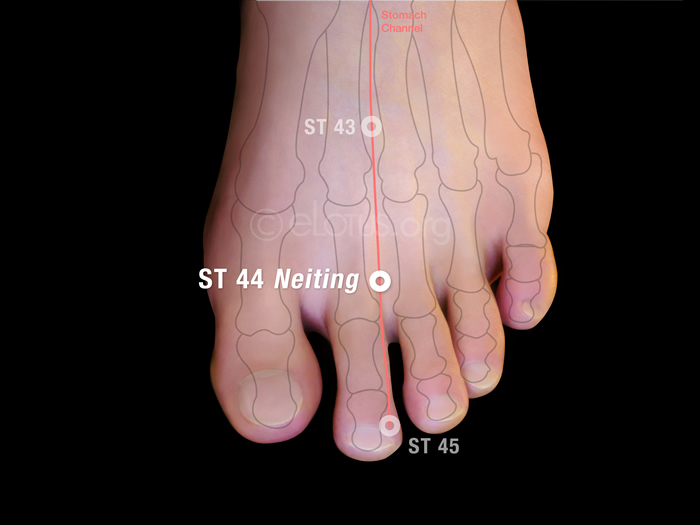
\includegraphics[width=\linewidth]{ST_44.jpg}
    }
    \\ \hline
    & & & & {\
        Hợp Cốc (Khác bên)
        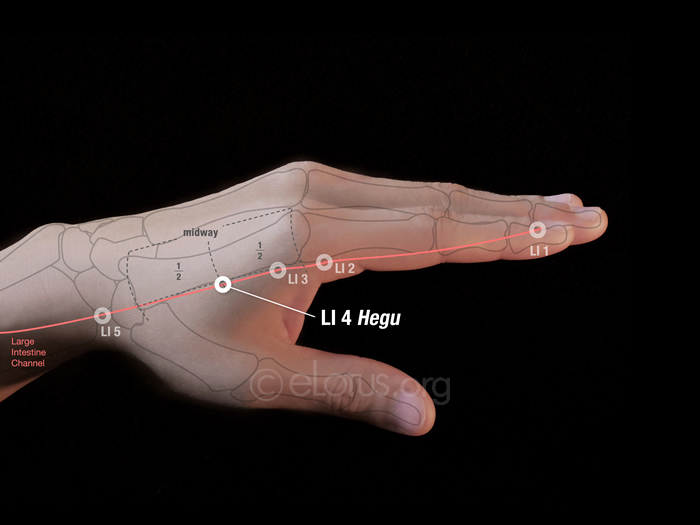
\includegraphics[width=\linewidth]{LI_4.jpg}
    }
    \\ \hline
    & & & & {\
        Thừa Tương (CV 24)
        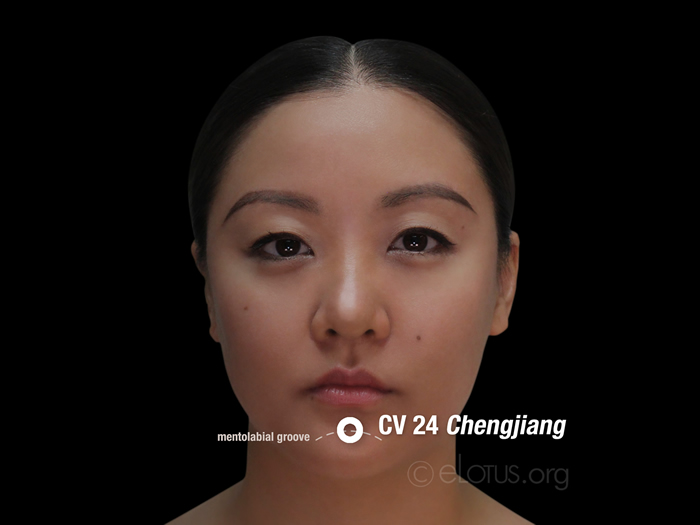
\includegraphics[width=\linewidth]{CV 24.jpg}

        Nằm ở chỗ lõm dưới môi dưới và phía trên cằm, tại chính giữa rãnh môi - cằm.
    }
    \\ \hline
    & & & & {\
        Địa Thương (ST 4)
        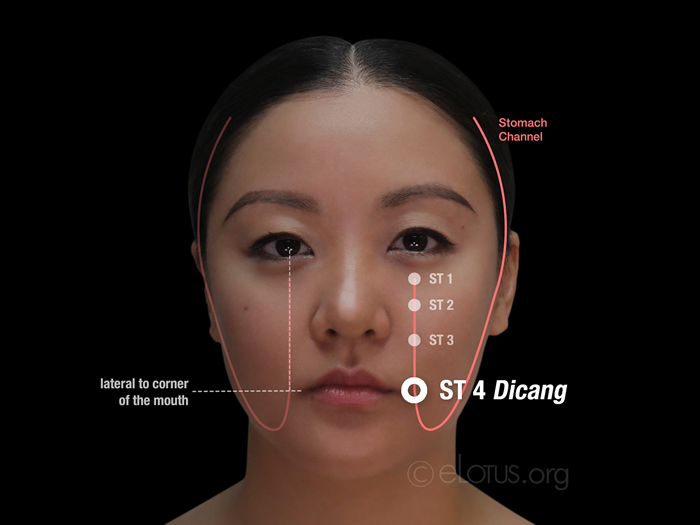
\includegraphics[width=\linewidth]{ST 4.jpg}

        Huyệt này nằm cách góc miệng (khoé miệng) 0,4 thốn về phía ngoài.
        Huyệt này nằm trên rãnh mũi - má (nếu bình thường không nhìn rõ, mỉm cười sẽ giúp thấy rõ hơn).
    }
    \\ \hline
    & & & & {\
        Nghinh Hương (LI 20)
        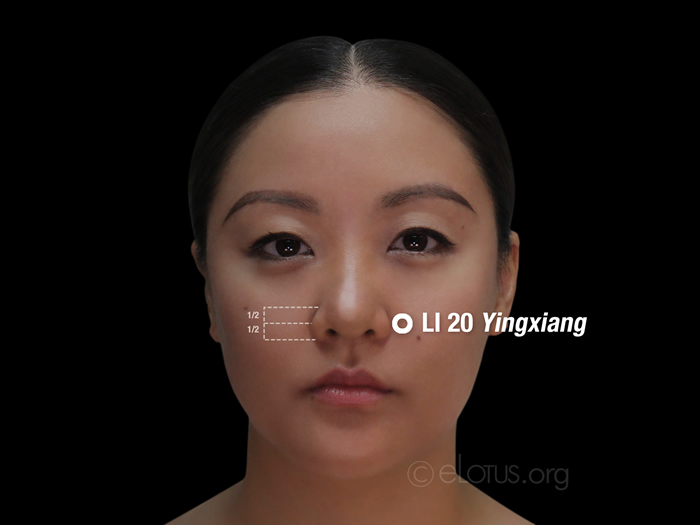
\includegraphics[width=\linewidth]{LI 20.jpg}

        Huyệt này nằm ở điểm giữa bờ ngoài của cánh mũi, trong rãnh mũi - má.
    }
    \\ \hline
    & & & & {\
        Nhân Trung (GV 26)
        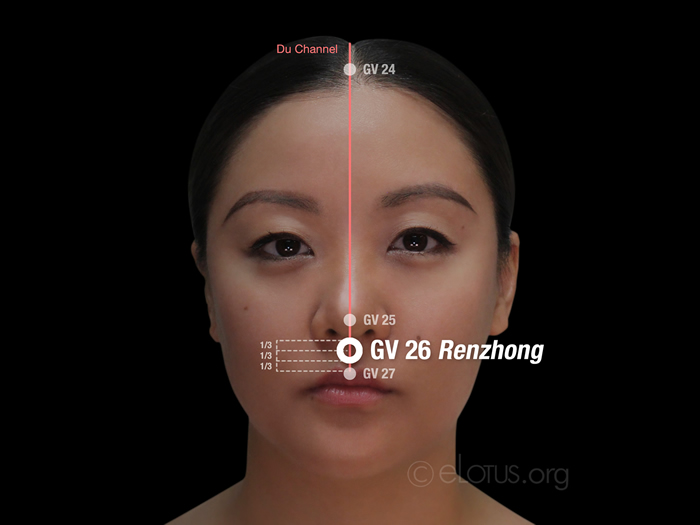
\includegraphics[width=\linewidth]{GV 26.jpg}

        Nằm ở vị trí 2/3 phía trên bờ môi trên, trên rãnh nhân trung và
        đường giữa mặt.
        Rãnh nhân trung là chỗ lõm nằm trên đường giữa mặt, nằm giữa mũi
        và bờ môi trên.
    }
    \\ \hline
    & & & & {
        Giáp Xa (ST 6)
        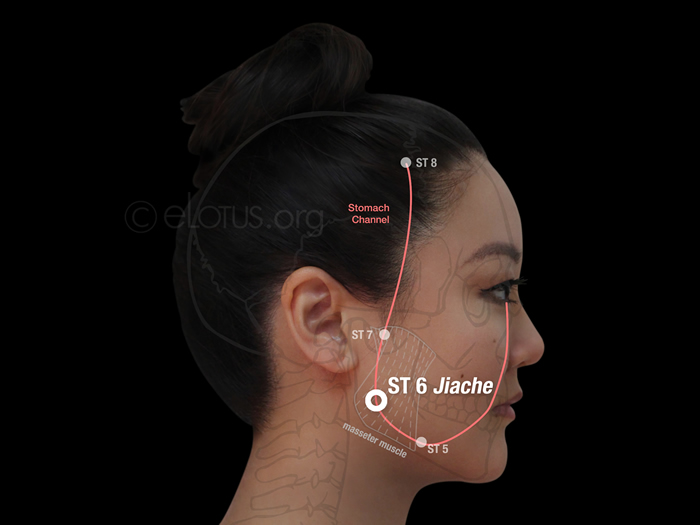
\includegraphics[width=\linewidth]{ST 6_1_0.jpg}
        \newline
        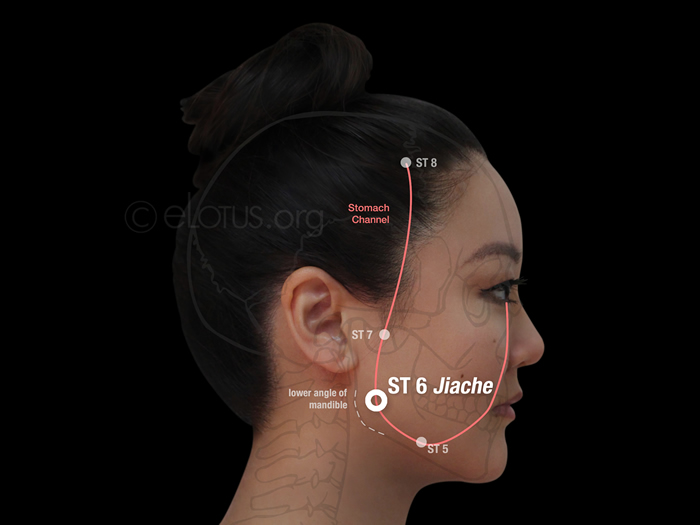
\includegraphics[width=\linewidth]{ST 6_2.jpg}

        Huyệt này nằm ở phía trước và phía trên góc hàm khoảng 1 chiều ngang ngón tay, nằm trên cơ cắn.

        Cơ cắn sẽ nổi rõ hơn khi cắn chặt răng (cắn hàm).
    }
    \\ \hline
    & & & & {\
        Hạ Quan (ST 7)
        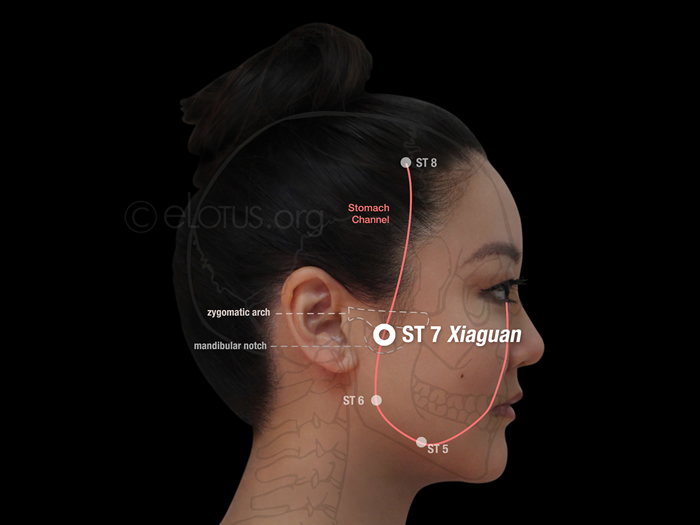
\includegraphics[width=\linewidth]{ST 7.jpg}
        Huyệt này nằm ở chỗ lõm tại bờ dưới gò má (cung gò má),
        phía trước lồi cầu xương hàm dưới.

        Có thể xác định huyệt bằng cách há miệng và đặt ngón tay
        lên lồi cầu xương hàm dưới, khi ngậm miệng lại ngón tay
        sẽ trượt vào đúng vị trí của huyệt ST-7 (khi châm cứu
        được thực hiện lúc ngậm miệng).
    }
    \\ \hline
    & & & & {\
        Ế Phong (TH 17)
        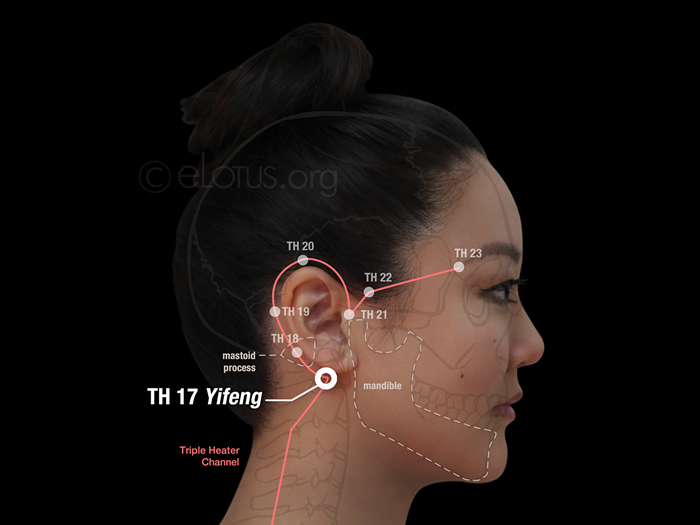
\includegraphics[width=\linewidth]{TH 17.jpg}
        Huyệt này nằm ở chỗ lõm phía sau dái tai, trung điểm giữa
        mỏm chũm và ngành lên xương hàm dưới, ngay phía trên mỏm ngang
        của đốt sống cổ C1 (đốt sống cổ thứ nhất).
        Dễ xác định huyệt hơn khi ép (gập) dái tai về phía trước.
    }
    \\ \hline
    & & & & {\
        Tình Minh (BL 1)
        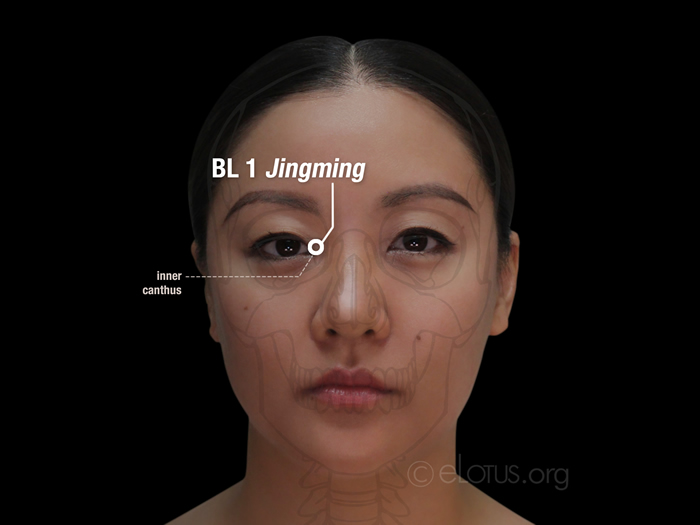
\includegraphics[width=\linewidth]{BL 1.jpg}
        Huyệt này nằm ở vị trí phía trên và trong khóe mắt
        trong 0,1 thốn, sát bờ trong xương hốc mắt.
    }
    \\ \hline
    & & & & {\
        Thừa Khấp (ST 1)
        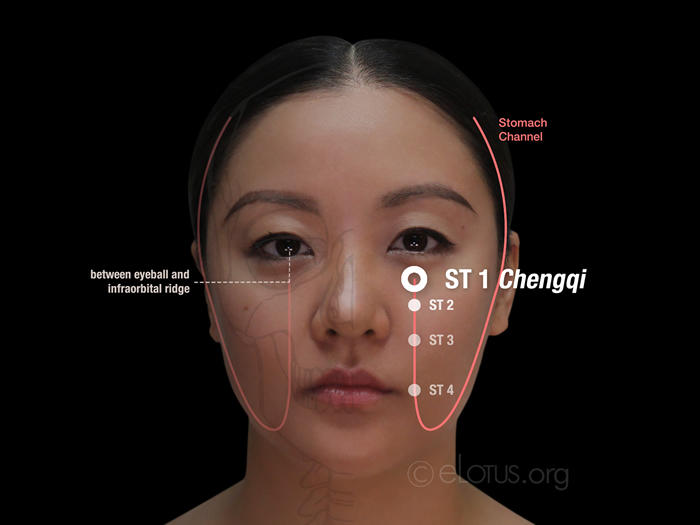
\includegraphics[width=\linewidth]{ST 1.jpg}
        Huyệt này nằm ngay phía dưới đồng tử (khi mắt nhìn thẳng về phía trước),
        ở khoảng giữa nhãn cầu và bờ dưới hốc mắt.
    }
    \\ \hline
    & & & & {\
        Đồng Tử Liêu (GB 1)
        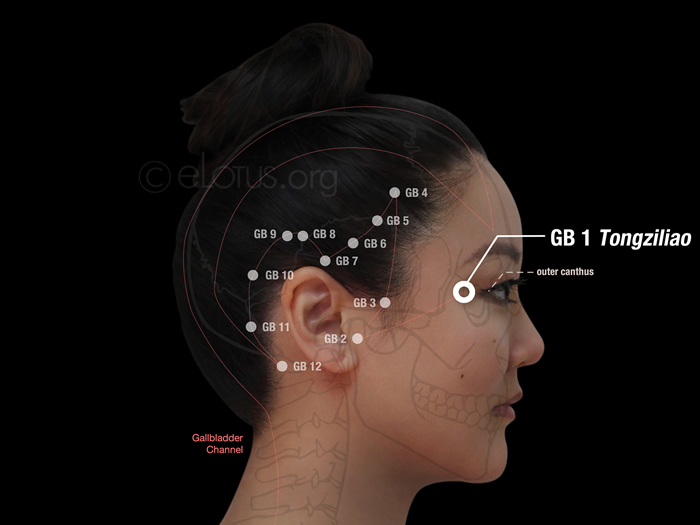
\includegraphics[width=\linewidth]{GB 1.jpg}
        Huyệt này nằm cách khóe mắt ngoài 0,5 thốn về phía bên (ngoài), nằm trong
        chỗ lõm phía ngoài của bờ xương hốc mắt.
    }
    \\ \hline
    & & & & {\
        Ty Trúc Không (TH 23)
        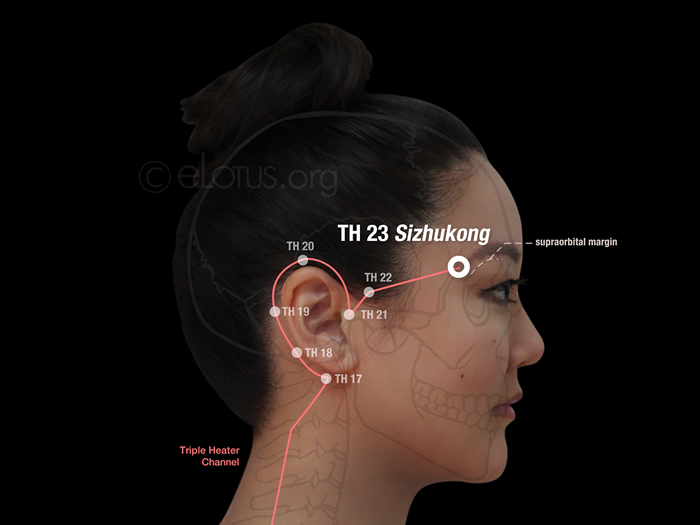
\includegraphics[width=\linewidth]{TH 23.jpg}
        Nằm ở chỗ lõm tại đuôi lông mày, ngay trên bờ trên hốc mắt.
    }
    \\ \hline
    & & & & {\
        Ngư Yêu (Ex-HN4)
        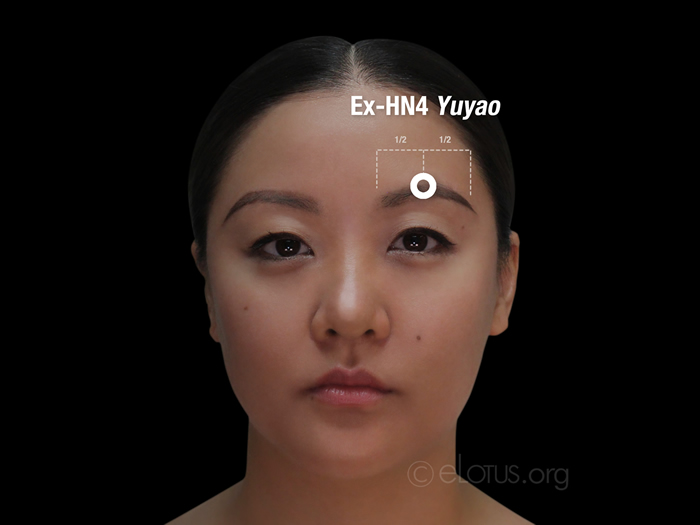
\includegraphics[width=\linewidth]{Ex-HN4.jpg}

        Nằm ở chính giữa lông mày, thẳng hàng với con ngươi (khi mắt nhìn thẳng về phía trước).
    }
    \\ \hline
    & & & & {\
        Toản Trúc (BL 2)
        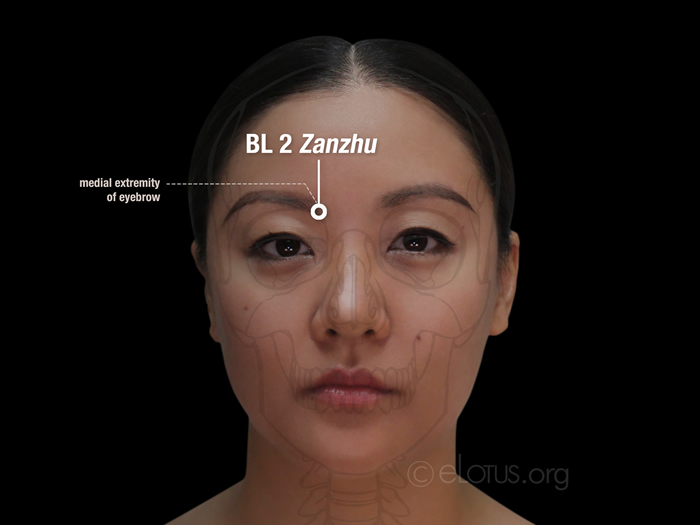
\includegraphics[width=\linewidth]{BL 2.jpg}
        Huyệt này nằm ở đầu trong lông mày, thẳng ngay phía trên huyệt BL-1
        (Tình Minh), trong chỗ lõm ở khuyết trên hốc mắt.
    }
    \\ \hline
    & & & & {\
        Dương Bạch (GB 14)

        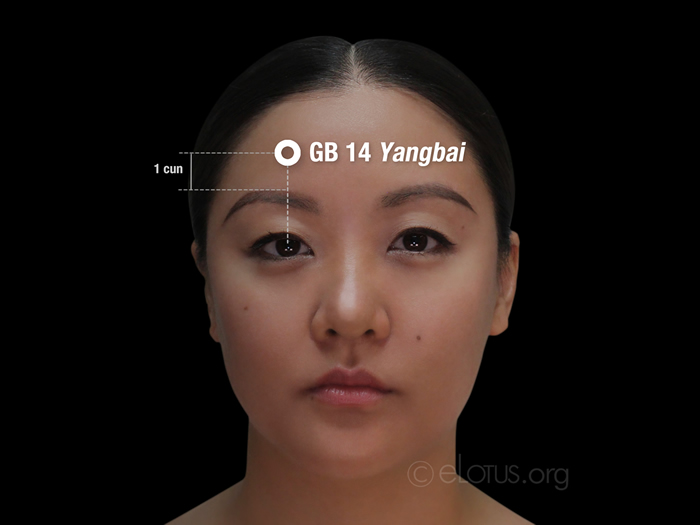
\includegraphics[width=\linewidth]{GB 14.jpg}

        Huyệt này nằm thẳng phía trên con ngươi (khi nhìn thẳng về phía trước)
        và cách điểm giữa lông mày lên phía trên 1 thốn.
    }
    \\ \hline
    10 & Đẩy & Toàn Trúc & &
    \\ \hline
    11 & Miết ngược & & &
    \\ \hline
    12 & Đẩy & Rãnh cười & &
    \\ \hline
\end{longtblr}

\subsubsection{Liệu trình}

\begin{itemize}
    \item Tần suất: ngày 1 lần; mỗi lần gần 30 phút làm đến khi khỏi.
    \item Lấy bên liệt làm chủ nhưng không bỏ qua bên lành.
    \item Giai đoạn đầu: chú trọng bảo vệ - trị mắt, tránh lộ đồng tử kéo dài gây khô/viêm giác mạc - kết mạc.
    \item Khuyên đeo kính râm bảo vệ mắt khi ra ngoài.
\end{itemize}

% \subsection{Liệt nửa người}
\subsubsection{Xoa bóp tay}
\begin{longtblr}[
    caption = {Liệt nửa người - Xoa bóp tay},
]{
    width = \textwidth,
    colspec = {| X[1,c] |X[1, c]|X[2, c]|X[1, c]|X[7, l]|},
    % hlines,
    rowhead = 1,
}
        \hline
        ID & Động tác & Vùng tác động & Số lần & Huyệt
        \\ \hline
        1 & Day & Vai xuống bàn tay & 3 &
        \\ \hline
        2 & Lăn & Cẳng tay đến vai & 3 &
        \\ \hline
        3 & Bóp & Cẳng tay đến vai & 3 &
        \\ \hline
        4 & Vờn & Tay & 3 &
        \\ \hline
        5 & Bấm & Huyệt & 1 & {
            Kiên Tỉnh, Kiên Ngung, Khúc Trì, Hợp Cốc, Dương Trì.
        }
        \\ & & & & {
            Kiên Tỉnh

            \kientinh
        }
        \\ & & & & {
            Kiên Ngung

            \kienngung
        }
        \\ & & & & {
            Khúc Trì

            \khuctri
        }
        \\ & & & & {
            Hợp Cốc

            \hopcoc
        }
        \\ & & & & {
            Dương Trì
            
            \duongtri
        }
        \\ \hline
        6 & Vê & Ngón tay & ? &
        \\ \hline
        7 & Vận động & Khớp vai, khuỷu tay, cổ tay và ngón tay & ? &
        \\ \hline
        8 & Rung & Tay & ? &
        \\ \hline
        9 & Phát & Vai xuống cẳng tay & 1 & Phát mạnh
        \\ \hline
    \end{longtblr}

\subsubsection{Xoa bóp chân}

\begin{longtblr}[
    caption = {Liệt nửa người - Xoa bóp chân},
]{
    width = \textwidth,
    colspec = {| X[1,c] |X[1, c]|X[2, c]|X[1, c]|X[7, l]|},
    % hlines,
    rowhead = 1,
}
    \hline
    ID & Động tác & Vùng tác động & Số lần & Huyệt
    \\ \hline
    1 & Day & Mông xuống cẳng chân & 3 &
    \\ \hline
    2 & Lăn & Mông xuống cẳng chân & 3 &
    \\ \hline
    3 & Bóp & Mông xuống cẳng chân & 3 & 
    \\ \hline
    4 & Bấm & Huyệt & 1 & {
        Hoàn Khiêu, Ân Môn, Thừa Phủ, Uỷ Trung,
        Thừa Sơn, Côn Lôn, Phong Thị, Dương Lăng Tuyền,
        Huyền Chung (Tuyệt Cốt), Giải Khê
    }
    \\ & & & & {
        Hoàn Khiêu

        \hoankhieu
    }
    \\ & & & & {
        Ân Môn
        
        \anmon
    }
    \\ & & & & {
        Thừa Phủ

        \thuaphu
    }
    \\ & & & & {
        Uỷ Trung

        \uytrung
    }
    \\ & & & & {
        Thừa Sơn

        \thuason
    }
    \\ & & & & {
        Côn Lôn

        \conlon
    }
    \\ & & & & {
        Phong Thị

        \phongthi
    }
    \\ & & & & {
        Dương Lăng Tuyền

        \duonglangtuyen
    }
    \\ & & & & {
        Huyền Chung

        \huyenchung
    }
    \\ & & & & {
        Giải khê

        \giaikhe
    }
    \\ \hline
    5 & Vận động & Khớp háng, khớp gối, khớp cổ chân và ngón chân & 1 &
    \\ \hline
    6 & Vê & Ngón chân & ? &
    \\ \hline
    7 & Vận động & Chân & ? &
    \\ \hline
    8 & Phát & Chân & 1 &
    \\ \hline
\end{longtblr}

\subsubsection{Xoa bóp lưng}

\begin{longtblr}[
    caption = {Liệt nửa người - Xoa bóp chân},
]{
    width = \textwidth,
    colspec = {| X[1,c] |X[1, c]|X[2, c]|X[1, c]|X[7, l]|},
    % hlines,
    rowhead = 1,
}
    \hline
    ID & Động tác & Vùng tác động & Số lần & Huyệt
    \\ \hline
    1 & Day & Vai tới mông & 3 &
    \\ \hline
    2 & Lăn & Vai tới mông & 3 &
    \\ \hline
    3 & Bóp & Vai tới mông & 3 &
    \\ \hline
    4 & Bấm & Huyệt & 1 & {
        hoa đà giáp tích bên liệt, cao hoang, thiên tông, cách du, thận du, đại trường du.
    }
    \\ & & & & {
        Giáp tích

        \giaptich
    }
    \\ & & & & {
        Cao hoang

        \caohoang
    }
    \\ & & & & {
        Thiên tông

        \thientong
    }
    \\ & & & & {
        Cách du

        \cachdu
    }
    \\ & & & & {
        Thần du

        \thandu
    }
    \\ & & & & {
        Đại trường du

        \daitruongdu
    }
    \\ \hline
    5 & Vận động & Cột sống & ? &
    \\ \hline
    6 & Phát & Lưng & 1 &
    \\ \hline
\end{longtblr}


% 
\subsection{Mất ngủ}

\begin{longtblr}[
    caption = {Mất ngủ},
]{
    width = \textwidth,
    colspec = {| X[1,c] |X[1, c]|X[2, c]|X[1, c]|X[7, l]|},
    % hlines,
    rowhead = 1,
}
    \hline
        ID & Động tác & Vùng tác động & Số lần & Huyệt
        \\ \hline
        1 & Bấm & Huyệt & 1 & {
            Thần môn

            \thanmon
        }
        \\ \hline
        2 & Bấm & Huyệt & 1 & {
            Ấn Đường

            \anduong
        }
        \\ \hline
        3 & Bấm & Huyệt & 1 & {
            Dũng Tuyền

            \dungtuyen
        }
        \\ \hline
        4 & Bấm & Huyệt & 1 & {
            Nội Quan

            \noiquan
        }
        \\ \hline
        5 & Bấm & Huyệt & 1 & {
            Tam Âm Giao

            \tamamgiao
        }
        \\ \hline
        6 & Bấm & Huyệt & 1 & {
            Phong Trì

            \phongtri
        }
        \\ \hline
    \end{longtblr}



\section{Tĩnh công của đại nhạn khí công}

\subsection{Nhận thức đúng đắn về mục đích ý nghĩa của việc luyện tập tĩnh công.}

Đại nhạn tĩnh công là một bộ phận cấu thành quan trọng trong cả bộ công pháp của môn phái Côn Luân Đạo gia. Trên cơ sở luyện thành thục động công, kết hợp luyện tập tĩnh công, có thể tiến tới điều động được nội khí, sơ thông kinh mạch, đạt được mục đích chữa bệnh, bồi bổ sức khỏe.

Tĩnh công trong Đại nhạn khí công lấy tĩnh làm chủ, trong tĩnh có động, ngoài tĩnh trong động. Trong quá trình luyện tập, nếu nắm được phương pháp đạo dẫn bằng hình thể và ý niệm một cách chuẩn xác thì hiệu quả luyện công rất rõ rệt, có thể thông suốt chu thiên một cách nhanh chóng; có thể hình thành chu thiên một cách tự nhiên. Tiểu chu thiên có thể đi xuôi, tức là khí đi từ Nhâm mạch sang Đốc mạch đi lên. Nhưng khi luyện công, không được có tạp niệm, quá trình luyện công xuất hiện ảo giác thì đừng cuống, phải nhìn nhận đúng đắn theo mục đích luyện công. Tựu chung, luyện kỹ tĩnh công, sẽ thu được những hiệu quả mà động công của Đại nhạn khí công không thể nào đạt được, thật kỳ diệu vô cùng.


\subsection{Giới thiện vài phương pháp và hình thức luyện tĩnh công đạt hiệu quả.}

Tĩnh công của Đại nhạn khí công có các tư thế lập (đứng), hành (đi), tọa (ngồi), ngọa (nằm) nhưng trong thực tiễn thường lấy tọa công làm công pháp chủ yếu. Trong tọa công lại phân biệt ngồi buông xuôi cẳng chân và ngồi khoanh tròn chân. Xin lần lượt trình bày 5 phương pháp tọa công của tĩnh công.

\subsubsection{Phương pháp trầm khí tự nhiên}

Ngồi đặt mông trên ghế 3 thốn, để lộ \textbf{Hội âm} ra,
thân trên và đùi tạo thành góc 90 hoặc lớn hơn,
đùi và cẳng chân tạo thành góc 90 hoặc lớn hơn,
hai bàn chân song song, rộng ngang vai, cổ để thẳng,
đầu lưỡi đặt lên vòm hàm trên, khép răng nhẹ nhẹ,
miệng hơi khép, hô hấp tự nhiên. Thả lỏng toàn thân,
sau đó hai tay bồng khí, từ trên đầu quán khí xuống dưới,
khí chìm xuống \textbf{Hạ Đan điền} hoặc \textbf{Dũng tuyền},
tiếp đó hạ mí mắt xuống, mắt từ từ nhìn xuống, vào chóp mũi
rồi sau đó nhìn xuống Đản trung, tiếp theo nhìn vào 
trong xuống đến \textbf{Hạ Đan điền}. Hai mắt khép nhẹ,
gạt bỏ hết mọi tạp niệm, không mảy may vấn vương về bất
cứ một điều gì kể cả bản thân mình. Hai lòng bàn tay đặt
lên huyệt \textbf{Lương khâu}, ngón tay cái đặt nhẹ trên
huyệt \textbf{Huyết hải}, bắt đầu tập công (hình 7-1).

\subsubsection{Phương pháp niệm thần}

Phương pháp này chủ yếu giúp cho những người mới tập tĩnh công chưa thể thả lỏng nhập tĩnh, để đi vào trạng thái khí công. Nói chung người mới luyện công thường rất khó tập trung tư tưởng, hễ nhắm mắt lại là suy nghĩ miên man, đủ thứ về cuộc sống, công việc, học hành, quan hệ đồng nghiệp v.v... Mà tư tưởng đã không yên thì không thể luyện tĩnh công có kết quả. Khi đó có thể dùng biện pháp niệm thầm trong đầu niệm hai chữ "công... thành." Niệm hai chữ "công thành" là cách niệm cơ bản của môn phái Côn Luân Đạo gia. Bằng cách này có thể giúp những người mới luyện tĩnh công từ bỏ những tư tưởng vấn vương, đi vào tùng tĩnh, kết quả giống như bài tập trầm khí tự nhiên (xem hình 8-1).

\subsubsection{Phương pháp điều túc}

Tư thế và yếu lĩnh động tác như bài tập trầm khí tự nhiên. Sau khi nhập tĩnh, dùng phương pháp hô hấp bụng thuận, tức là khi hít vào thì phình bụng dưới lên, thở ra thì thu bụng dưới. Cũng có thể dùng phương pháp thở bụng nghịch để tiếp vào trạng thái khí công. Trong quá trình luyện công trình độ thở cao nhất là đạt được "Thai túc pháp".

Khi hô hấp bằng mũi phải tự nhiên, thông suốt, đạt đến trình độ thở bụng sâu, dài, đều, mịn, kỵ nhất là cách thở ngực, nông, ngắn, gấp, thở hồng hộc (hình 8-1).

\subsubsection{Phương pháp tán khí}

Phương pháp này chỉ có thể tiến hành luyện tập trên cơ sở đã luyện 3 phương pháp trên, đã thông suốt tiểu chu thiên, đã nắm vững sự vận hành của khí. Nội dung của phương pháp là điều khiển


tập trung nội khí, khí chu thiên đến bộ phận có bệnh, dùng ý niệm xua tan bệnh khí trong
 cơ thể, làm thân thể khỏe mạnh, thoải mái. Khi tập phương pháp này,
 trong quá trình luyện công có dùng một chút ý niệm, tức là dùng ý niệm đạo dẫn để thực
  hiện cách luyện công này (hình 8-1).

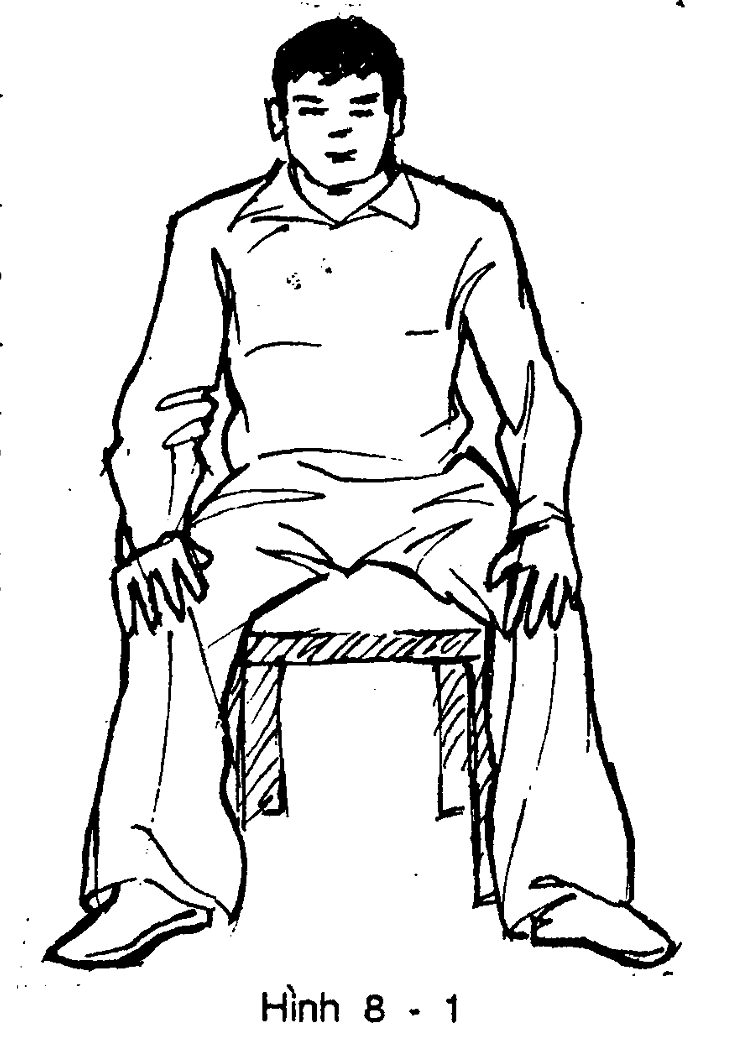
\includegraphics[width=0.5\textwidth]{qigong8.1.png}

\subsubsection{Phương pháp luyện chu thiên ngoài cơ thể}

Tư thế và yếu lĩnh làm như phép trầm khí tự nhiên. Khi luyện công, thông qua thể hình và dùng ý niệm đạo dẫn, thải những khí vẩn đục ra ngoài cơ thể, sau đó quán khí của đại tự nhiên thấu vào cơ thể thông qua huyệt Bách hội, hoặc Đại chùy. Làm như vậy sẽ tạo được vòng tuần hoàn lớn giữa ngoài và trong cơ thể. Khi luyện công bằng phương pháp thứ tư và thứ năm, đòi hỏi phải có công cơ bản thật vững chắc, công phu đã khá lên nhiều thì mới có thể luyện phương pháp "Chu thiên ngoài cơ thể".

Cách thu công của 5 phương pháp trên đều là: hợp hai bàn tay, xoa bàn tay 7 lần, sau đó dùng ngón tay hoặc lòng bàn tay xoa ấn mắt 7 lần, dùng hai bàn tay chải đầu một cách tự nhiên, dần dần mở mắt. Sau đó hai tay bồng khí đưa lên đằng trước phía trên đầu, quán khí vào Thượng, Trung Hạ Đan điền, ngồi một lát rồi mới có thể đứng dậy hoạt động như hình 8-1 .

Ngoài tĩnh công ngồi thả chân như đã trình bày ở trên còn có cả cách ngồi khoanh tròn chân; yếu lĩnh thân trên ngay thẳng. Đầu lưỡi đặt lên vòm hàm trên, răng khép nhẹ, miệng hơi hé, bàn chân trái khoanh vào trong, đặt dưới đùi phải, chân phải xếp khoanh ở ngoài, bàn chân để ở dưới đùi chân trái, thành khoanh chân tự do, hai lòng bàn tay đặt nhẹ huyệt Lương khâu trên đầu gối, ngón tay

cái điểm nhẹ trên huyệt Huyết hải, vai phải thả lỏng, hai cánh tay tròn, luyện công trong trạng thái không mảy may vấn vương về điều gì, kể cả sự tồn tại của bản thân.

Không quy định thời gian một lần luyện tĩnh công là bao nhiêu, người mới tập có thể tập thời gian ngắn, có thể tập khoảng 10 phút. Công phu càng sâu thì thời gian tập có thể kéo dài dần đến 30 phút. Nếu hoàn cảnh cho phép, có thể tập một giờ hoặc lâu hơn. Nếu điều kiện không cho phép, có thể luyện ít cũng được. Cái chính là tập xong phải cảm thấy thoải mái.

\subsection{Những điều cần chú ý khi luyện tĩnh công}

\subsubsection{Để luyện Đại nhạn khí công đạt kết quả, nhất định phải quán xuyến suốt quá trình luyện công những yêu cầu: "tĩnh, tùng, không".}

\begin{itemize}
    \item \textbf{Tĩnh:} Nghĩa là yên tĩnh, môi trường luyện công phải yên tĩnh, không khí phải yên lành, thể hình phải "Điềm đạm hư vô".
    \item \textbf{Tùng:} Nghĩa là phải thả lỏng cả tư tưởng, cơ bắp, và các khớp xương.
    \item \textbf{Không:} Tức là người luyện công không suy nghĩ gì cả. Khi luyện công nhìn thấy bất cứ cái gì cũng coi như không thấy, nghe thấy bất cứ cái gì cũng coi như không nghe, nhất định phải đạt được yêu cầu "không có gì cả, không có ai cả".
\end{itemize}

\subsubsection{Khi luyện công, cần tránh sự quấy nhiễu của thất tình (bảy loại tình cảm) và Lục dâm}

Bảy thứ tình cảm: vui, cáu giận, lo lắng, suy nghĩ, bi ai, sợ hãi, kinh hoàng, là những yếu tố dẫn bệnh vào cơ thể. Còn lục dâm là: phong, hàn, thử, thấp, táo, hỏa, chúng cũng là những yếu tố khách quan dẫn bệnh đến cơ thể. Tuy vậy ý thức chủ quan của con người có thể khống chế được chúng.

Quá vui thì tổn thương đến tâm, cáu giận thì hại đến gan, quá lo lắng phiền muộn thì hại đến vị, suy nghĩ quá mức thì hại đến tỳ, sợ hãi thì hại đến đởm, kinh hoàng thì hại thận. Nên phải dùng ý thức chủ quan để khắc phục những nhân tố khách quan có thể quấy nhiễu việc luyện công. Ngoài ra cần chú ý khi gặp sấm chớp, mưa to thì không luyện công.

\subsubsection{Khi luyện công cần chú ý}

Khởi cư hữu thường, \\
Ẩm thực thích độ, \\
Tiết chế phòng sự \\
Bất vong lao tác:

Theo ngôn ngữ hiện đại thì lời nói trên của người xưa có nghĩa là:

\textit{"Khởi cư hữu thường"}: sinh hoạt trong ngày phải có nề nếp, kể cả việc thức ngủ, cũng cần phải tuân theo quy luật.

\textit{"Ẩm thực thích độ"}: hàng ngày luyện công, không nên ăn quá no, cũng không nên luyện công khi đói. Không nên ăn quá ngon (ăn cá, thịt nhiều quá), tuy vậy cũng cần phải chú ý dinh dưỡng đầy đủ, thích hợp khẩu vị, ăn nhiều rau, đậu. Không luyện công trước và sau bữa ăn 30 phút.

\textit{"Tiết chế phòng sự"}: cần hạn chế sinh hoạt vợ chồng để khỏi bị ảnh hưởng kết quả luyện công. Lấy lời dạy của
người xưa: "Xuân nhất, thu nhị, hạ tam, đông tàng" để tiết chế sinh hoạt vợ chồng.

\textit{"Bất vong lao tác"}: người già và những người lao động trí óc phải tham gia lao động chân tay phù hợp với sức khỏe, với điều kiện của bản thân. Làm như vậy không những củng cố được thành quả luyện công, mà còn có thể giữ gìn sức khỏe, kéo dài tuổi thọ. Tóm lại "Động tĩnh lạc thọ (Sự sống tồn tại trong sự vận động)", ý nghĩa chính là ở chỗ đó.

\subsubsection{Mặc khi luyện tĩnh công}

Phải mặc quần áo rộng, thoải mái, không nên mặc chặt quá, nếu không sẽ ảnh hưởng đến việc hành khí. Ngoài ra, trước khi luyện công, nếu không mót đái, mót ỉa thì không nên cố vào nhà xí để tránh ảnh hưởng đến việc thả lỏng, nhập tĩnh.

\subsubsection{Gặp chuyện lạ khi luyện công}

Nếu bị kinh hoàng thì không nên vội mở mắt, không nên vội đứng dậy mà bình tĩnh theo yếu lĩnh thu công, dần dần thu công lại, sau đó mới đứng dậy đi để tránh bị choáng, bị tức ngực.

Còn một phương pháp luyện tĩnh công nữa tên là:

\textbf{"Tĩnh tọa thải độc công"} (hình 8-2)

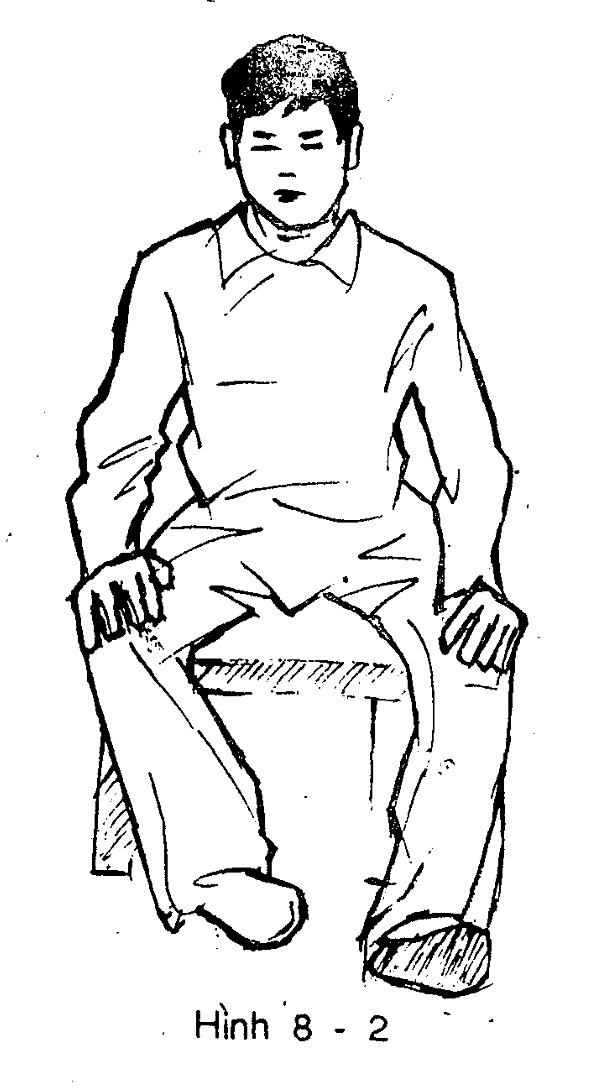
\includegraphics[width=0.5\textwidth]{qigong8.2.png}

\textit{Phương pháp tập:} thả lỏng, nhập tĩnh. Sau khi ngồi ở ghế, chân trái hơi gập để ở đằng trước, mép ngoài chân trái tiếp đất, mũi chân hướng ra đằng trước. Chân phải cong ở đằng sau, mép ngoài chân phải tiếp đất, mũi chân đối chuẩn với gót chân trái. Hai bàn chân cách nhau khoảng 7 thốn. Lòng bàn tay trái chiếu chuẩn vào huyệt Dương lăng tuyền, lòng bàn tay phải đối chuẩn với huyệt Lương khâu chân phải, nhưng hai bàn tay và tay đều không áp sát vào người, cách thân khoảng một thốn là được. Nếu tay có cảm giác mỏi thì có thể áp sát vào huyệt vị mà lòng bàn tay chiếu vào, luyện đến khi có cảm giác khoan khoái thì bỏ ra, rồi lại tiếp tục làm. Khi luyện công phải thêm ý để đạo dẫn, tức là niệm thầm câu "Bệnh khí nhập thổ, độc khí nhập thổ". Yếu lĩnh còn lại làm như phương pháp trầm khí tự nhiên.

% \section{Huyệt}

\section{LU 7 -- Liệt khuyết (Lieque)}

\subsection{Vị trí huyệt}

Huyệt Liệt khuyết nằm ở mặt quay của cẳng tay, cách nếp gấp ngang cổ tay khoảng \(1{,}5\) thốn về phía gần khuỷu tay, trong khe giữa gân cơ cánh tay quay và gân cơ dạng dài ngón cái.

Có thể xác định huyệt bằng cách đan chéo ngón trỏ và ngón cái của hai bàn tay, đặt ngón trỏ của một bàn tay lên mỏm trâm quay của bàn tay còn lại. Huyệt nằm tại chỗ lõm ngay dưới đầu ngón trỏ.

\begin{figure}[htbp]
    \centering
    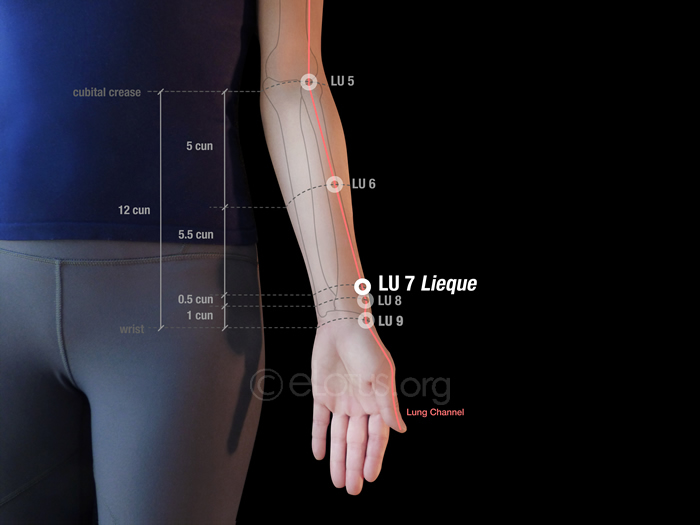
\includegraphics[width=0.65\textwidth]{LU_7.jpg}
    \caption{Huyệt Liệt khuyết (LU 7).}
    \label{fig:lu7}
\end{figure}

\subsection{Chỉ định}

Các chỉ định được liệt kê trong tài liệu nguồn bao gồm:

\begin{itemize}
    \item Ho, hen suyễn và đau họng.
    \item Đau đầu, đau nửa đầu và cứng cổ.
    \item Liệt mặt và đau răng.
    \item Đau và yếu vùng cổ tay.
\end{itemize}

\subsection{Cơ chế tác dụng theo y học cổ truyền}

Theo lý luận y học cổ truyền, huyệt Liệt khuyết có các tác dụng sau:

\begin{itemize}
    \item Giải biểu, khu phong.
    \item Tuyên thông Phế khí, thúc đẩy chức năng túc giáng của Phế.
    \item Khai thông và điều hòa mạch Nhâm.
    \item Điều hòa thủy đạo.
    \item Có lợi cho vùng đầu và cổ.
\end{itemize}

\subsection{Ứng dụng trong phương pháp Balance}

Trong phương pháp Balance, huyệt Liệt khuyết được liên hệ với các kinh mạch và hệ thống sau:

\begin{itemize}
    \item \textbf{Kinh thủ Thái âm -- Phế:} kinh mạch chủ quản của huyệt.
    \item \textbf{Hệ thống 1:} kinh túc Thái âm -- Tỳ.
    \item \textbf{Hệ thống 2:} kinh túc Thái dương -- Bàng quang.
    \item \textbf{Hệ thống 3:} kinh thủ Dương minh -- Đại trường.
    \item \textbf{Hệ thống 4:} kinh túc Thái dương -- Bàng quang.
    \item \textbf{Hệ thống 5:} kinh túc Quyết âm -- Can.
\end{itemize}

\subsection{Kỹ thuật châm cứu}

Theo tài liệu nguồn, kỹ thuật châm được mô tả như sau:

\begin{itemize}
    \item \textbf{Hướng châm:} châm chếch hướng lên phía khuỷu tay.
    \item \textbf{Độ sâu:} khoảng \(0{,}3\)--\(0{,}5\) thốn.
\end{itemize}

Hướng châm và độ sâu thực tế cần được điều chỉnh theo đặc điểm giải phẫu, thể trạng người bệnh và đánh giá của người hành nghề có chuyên môn.

\subsection{Đặc tính huyệt}

Theo phân loại trong tài liệu nguồn, Liệt khuyết có các đặc tính sau:

\begin{itemize}
    \item \textbf{Lạc huyệt:} kinh Phế.
    \item \textbf{Huyệt Xuất:} kinh Phế.
    \item \textbf{Huyệt phối:} mạch Âm Kiều (Yinqiao).
    \item \textbf{Huyệt chủ:} mạch Nhâm.
    \item \textbf{Huyệt chỉ huy:} vùng đầu và gáy.
\end{itemize}

\subsection{Tài liệu tham khảo}

Master Tung's Acupuncture. (n.d.). \textit{Lieque (LU 7)}.
eLotus CORE.
\url{https://www.mastertungacupuncture.org/acupuncture/traditional/points/lu7}
% 
\clearpage
\subsection{Lung Meridian (LU): Kinh thủ thái âm Phế}
\subsubsection{Zhongfu (LU 1): Trung Phủ}
\includegraphics[width=\linewidth]{"LU_1.jpg"}

\subsubsection{Yunmen (LU 2): Vân Môn}
\includegraphics[width=\linewidth]{"LU_2.jpg"}

\subsubsection{Tianfu (LU 3): Thiên Phủ}
\includegraphics[width=\linewidth]{"LU_3.jpg"}

\subsubsection{Xiabai (LU 4): Hiệp Bạch}
\includegraphics[width=\linewidth]{"LU_4.jpg"}

\subsubsection{Chize (LU 5): Xích Trạch}
\includegraphics[width=\linewidth]{"LU_5.jpg"}

\subsubsection{Kongzui (LU 6): Khổng Tối}
\includegraphics[width=\linewidth]{"LU_6.jpg"}

\subsubsection{Lieque (LU 7): Liệt Khuyết}
\includegraphics[width=\linewidth]{"LU_7.jpg"}

\subsubsection{Jingqu (LU 8): Kinh Cừ}
\includegraphics[width=\linewidth]{"LU_8.jpg"}

\subsubsection{Taiyuan (LU 9): Thái Uyên}
\includegraphics[width=\linewidth]{"LU_9.jpg"}

\subsubsection{Yuji (LU 10): Ngư Tế}
\includegraphics[width=\linewidth]{"LU_10.jpg"}

\subsubsection{Shaoshang (LU 11): Thiếu Thương}
\includegraphics[width=\linewidth]{"LU_11.jpg"}

% \clearpage
\subsection{Large Intestine Meridian (LI): Kinh thủ dương minh Đại trường}

\subsubsection{Shangyang (LI 1): Thương Dương}
\includegraphics[width=\linewidth]{"LI_1.jpg"}

\subsubsection{Erjian (LI 2): Nhị Gian}
\includegraphics[width=\linewidth]{"LI_2.jpg"}

\subsubsection{Sanjian (LI 3): Tam Gian}
\includegraphics[width=\linewidth]{"LI_3.jpg"}

\subsubsection{Hegu (LI 4): Hợp Cốc}
\includegraphics[width=\linewidth]{"LI_4.jpg"}

\subsubsection{Yangxi (LI 5): Dương Khê}
\includegraphics[width=\linewidth]{"LI_5.jpg"}

\subsubsection{Pianli (LI 6): Thiên Lịch}
\includegraphics[width=\linewidth]{"LI_6.jpg"}

\subsubsection{Wenliu (LI 7): Ôn Lưu}
\includegraphics[width=\linewidth]{"LI_7.jpg"}

\subsubsection{Xialian (LI 8): Hạ Liêm}
\includegraphics[width=\linewidth]{"LI_8.jpg"}

\subsubsection{Shanglian (LI 9): Thượng Liêm}
\includegraphics[width=\linewidth]{"LI_9.jpg"}

\subsubsection{Shousanli (LI 10): Thủ Tam Lý}
\includegraphics[width=\linewidth]{"LI_10.jpg"}

\subsubsection{Quchi (LI 11): Khúc Trì}
\includegraphics[width=\linewidth]{"LI_11.jpg"}

\subsubsection{Zhouliao (LI 12): Trửu Liêu}
\includegraphics[width=\linewidth]{"LI_12a_0.jpg"}

\subsubsection{Shouwuli (LI 13): Thủ Ngũ Lý}
\includegraphics[width=\linewidth]{"LI_13.jpg"}

\subsubsection{Binao (LI 14): Tý Nhu}
\includegraphics[width=\linewidth]{"LI_14.jpg"}

\subsubsection{Jianyu (LI 15): Kiên Ngung}
\includegraphics[width=\linewidth]{"LI_15b.jpg"}

\subsubsection{Jugu (LI 16): Cự Cốt}
\includegraphics[width=\linewidth]{"LI_16b.jpg"}

\subsubsection{Tianding (LI 17): Thiên Đỉnh}
\includegraphics[width=\linewidth]{"LI 17.jpg"}

\subsubsection{Futu (LI 18): Phủ Đột}
\includegraphics[width=\linewidth]{"LI 18.jpg"}

\subsubsection{Kouheliao (LI 19): Hòa Liêu}
\includegraphics[width=\linewidth]{"LI 19.jpg"}

\subsubsection{Yingxiang (LI 20): Nghinh Hương}
\includegraphics[width=\linewidth]{"LI 20.jpg"}


% \clearpage
\subsection{Stomach Meridian (ST): Kinh túc dương minh Vị}

\subsubsection{Chengqi (ST 1): Thừa Khấp}
\includegraphics[width=\linewidth]{"ST 1.jpg"}
Huyệt này nằm ngay phía dưới đồng tử (khi mắt nhìn thẳng về phía trước),
ở khoảng giữa nhãn cầu và bờ dưới hốc mắt.

\subsubsection{Sibai (ST 2): Tứ Bạch}
\includegraphics[width=\linewidth]{"ST 2.jpg"}

\subsubsection{Juliao (ST 3): Cự Liêu}
\includegraphics[width=\linewidth]{"ST 3.jpg"}

\subsubsection{Dicang (ST 4): Địa Thương}
\includegraphics[width=\linewidth]{"ST 4.jpg"}

\subsubsection{Daying (ST 5): Đại Nghinh}
\includegraphics[width=\linewidth]{"ST 5.jpg"}

\subsubsection{Jiache (ST 6): Giáp Xa}
\includegraphics[width=\linewidth]{"ST 6_1_0.jpg"}
\includegraphics[width=\linewidth]{"ST 6_2.jpg"}

\subsubsection{Xiaguan (ST 7): Hạ Quan}
\includegraphics[width=\linewidth]{"ST 7.jpg"}

\subsubsection{Touwei (ST 8): Đầu Duy}
\includegraphics[width=\linewidth]{"ST 8.jpg"}
\includegraphics[width=\linewidth]{"ST 8_2.jpg"}

\subsubsection{Renying (ST 9): Nhân Nghinh}
\includegraphics[width=\linewidth]{"ST 9.jpg"}

\subsubsection{Shuitu (ST 10): Thủy Đột}
\includegraphics[width=\linewidth]{"ST 10.jpg"}

\subsubsection{Qishe (ST 11): Khí Xá}
\includegraphics[width=\linewidth]{"ST 11.jpg"}

\subsubsection{Quepen (ST 12): Khuyết Bồn}
\includegraphics[width=\linewidth]{"ST 12.jpg"}

\subsubsection{Qihu (ST 13): Khí Hộ}
\includegraphics[width=\linewidth]{"ST 13.jpg"}

\subsubsection{Kufang (ST 14): Khố Phòng}
\includegraphics[width=\linewidth]{"ST 14.jpg"}

\subsubsection{Wuyi (ST 15): Ốc É}
\includegraphics[width=\linewidth]{"ST 15.jpg"}

\subsubsection{Yingchuang (ST 16): Ưng Song}
\includegraphics[width=\linewidth]{"ST 16.jpg"}

\subsubsection{Ruzhong (ST 17): Nhũ Trung}
\includegraphics[width=\linewidth]{"ST 17.jpg"}

\subsubsection{Rugen (ST 18): Nhũ Căn}
\includegraphics[width=\linewidth]{"ST 18.jpg"}

\subsubsection{Burong (ST 19): Bất Dung}
\includegraphics[width=\linewidth]{"ST 19.jpg"}

\subsubsection{Chengman (ST 20): Thừa Mãn}
\includegraphics[width=\linewidth]{"ST 20.jpg"}

\subsubsection{Liangmen (ST 21): Lương Môn}
\includegraphics[width=\linewidth]{"ST 21.jpg"}

\subsubsection{Guanmen (ST 22): Quan Môn}
\includegraphics[width=\linewidth]{"ST 22.jpg"}

\subsubsection{Taiyi (ST 23): Thái Ất}
\includegraphics[width=\linewidth]{"ST 23.jpg"}

\subsubsection{Huaroumen (ST 24): Hoạt Nhục Môn}
\includegraphics[width=\linewidth]{"ST 24.jpg"}

\subsubsection{Tianshu (ST 25): Thiên Khu}
\includegraphics[width=\linewidth]{"ST 25.jpg"}

\subsubsection{Wailing (ST 26): Ngoại Lăng}
\includegraphics[width=\linewidth]{"ST 26.jpg"}

\subsubsection{Daju (ST 27): Đại Cự}
\includegraphics[width=\linewidth]{"ST 27.jpg"}

\subsubsection{Shuidao (ST 28): Thủy Đạo}
\includegraphics[width=\linewidth]{"ST 28.jpg"}

\subsubsection{Guilai (ST 29): Quy Lai}
\includegraphics[width=\linewidth]{"ST 29.jpg"}

\subsubsection{Qichong (ST 30): Khí Xung}
\includegraphics[width=\linewidth]{"ST 30.jpg"}

\subsubsection{Biguan (ST 31): Bễ Quan}
\includegraphics[width=\linewidth]{"ST_31.jpg"}

\subsubsection{Futu (ST 32): Phục Thỏ}
\includegraphics[width=\linewidth]{"ST_32.jpg"}

\subsubsection{Yinshi (ST 33): Âm Thị}
\includegraphics[width=\linewidth]{"ST_33.jpg"}

\subsubsection{Liangqiu (ST 34): Lương Khâu}
\includegraphics[width=\linewidth]{"ST_34.jpg"}

\subsubsection{Dubi (ST 35): Độc Tỵ}
\includegraphics[width=\linewidth]{"ST_35.jpg"}

\subsubsection{Zusanli (ST 36): Túc Tam Lý}
\includegraphics[width=\linewidth]{"ST_36.jpg"}

\subsubsection{Shangjuxu (ST 37): Thượng Cự Hư}
\includegraphics[width=\linewidth]{"ST_37.jpg"}

\subsubsection{Tiaokou (ST 38): Điều Khẩu}
\includegraphics[width=\linewidth]{"ST_38.jpg"}

\subsubsection{Xiajuxu (ST 39): Hạ Cự Hư}
\includegraphics[width=\linewidth]{"ST_39.jpg"}

\subsubsection{Fenglong (ST 40): Phong Long}
\includegraphics[width=\linewidth]{"ST_40.jpg"}

\subsubsection{Jiexi (ST 41): Giải Khê}
\includegraphics[width=\linewidth]{"ST 41.jpg"}

\subsubsection{Chongyang (ST 42): Xung Dương}
\includegraphics[width=\linewidth]{"ST 42.jpg"}

\subsubsection{Xiangu (ST 43): Hãm Cốc}
\includegraphics[width=\linewidth]{"ST_43.jpg"}

\subsubsection{Neiting (ST 44): Nội Đình}
\includegraphics[width=\linewidth]{"ST_44.jpg"}

\subsubsection{Lidui (ST 45): Lệ Đoài}
\includegraphics[width=\linewidth]{"ST_45.jpg"}

% \clearpage
\subsection{Spleen Meridian(SP): Kinh túc thái âm Tỳ}

\subsubsection{Yinbai (SP 1): Ân Bạch}
\includegraphics[width=\linewidth]{"SP_1.jpg"}

\subsubsection{Dadu (SP 2): Đại Đô}
\includegraphics[width=\linewidth]{"SP_2.jpg"}

\subsubsection{Taibai (SP 3): Thái Bạch}
\includegraphics[width=\linewidth]{"SP_3.jpg"}

\subsubsection{Gongsun (SP 4): Công Tôn}
\includegraphics[width=\linewidth]{"SP_4.jpg"}

\subsubsection{Shangqiu (SP 5): Thương Khâu}
\includegraphics[width=\linewidth]{"SP_5.jpg"}

\subsubsection{Sanyinjiao (SP 6): Tam Âm Giao}
\includegraphics[width=\linewidth]{"SP_6.jpg"}

\subsubsection{Lougu (SP 7): Lậu Cốc}
\includegraphics[width=\linewidth]{"SP_7.jpg"}

\subsubsection{Diji (SP 8): Địa Cơ}
\includegraphics[width=\linewidth]{"SP_8.jpg"}

\subsubsection{Yinlingquan (SP 9): Âm Lăng Tuyền}
\includegraphics[width=\linewidth]{"SP_9.jpg"}

\subsubsection{Xuehai (SP 10): Huyết Hải}
\includegraphics[width=\linewidth]{"SP_10a.jpg"}

\subsubsection{Jimen (SP 11): Cơ Môn}
\includegraphics[width=\linewidth]{"SP_11.jpg"}

\subsubsection{Chongmen (SP 12): Xung Môn}
\includegraphics[width=\linewidth]{"SP 12.jpg"}

\subsubsection{Fushe (SP 13): Phủ Xá}
\includegraphics[width=\linewidth]{"SP 13.jpg"}

\subsubsection{Fujie (SP 14): Phúc Kết}
\includegraphics[width=\linewidth]{"SP 14.jpg"}

\subsubsection{Daheng (SP 15): Đại Hoành}
\includegraphics[width=\linewidth]{"SP 15.jpg"}

\subsubsection{Fuai (SP 16): Phúc Ai}
\includegraphics[width=\linewidth]{"SP 16.jpg"}

\subsubsection{Shidou (SP 17): Thực Đậu}
\includegraphics[width=\linewidth]{"SP 17.jpg"}

\subsubsection{Tianxi (SP 18): Thiên Khê}
\includegraphics[width=\linewidth]{"SP 18.jpg"}

\subsubsection{Xiongxiang (SP 19): Hung Hương}
\includegraphics[width=\linewidth]{"SP 19.jpg"}

\subsubsection{Zhourong (SP 20): Chu Vinh}
\includegraphics[width=\linewidth]{"SP 20.jpg"}

\subsubsection{Dabao (SP 21): Đại Bao}
\includegraphics[width=\linewidth]{"SP21.jpg"}

% \clearpage
\subsection{Heart Meridian (HT): Kinh thủ thiếu âm Tâm}

\subsubsection{Jiquan (HT 1): Cực Tuyền}
\includegraphics[width=\linewidth]{"HT1.jpg"}
\includegraphics[width=\linewidth]{"HT 1.jpg"}

\subsubsection{Qingling (HT 2): Thanh Linh}
\includegraphics[width=\linewidth]{"HT_2.jpg"}

\subsubsection{Shaohai (HT 3): Thiếu Hải}
\includegraphics[width=\linewidth]{"HT_3.jpg"}

\subsubsection{Lingdao (HT 4): Linh Đạo}
\includegraphics[width=\linewidth]{"HT_4.jpg"}

\subsubsection{Tongli (HT 5): Thông Lý}
\includegraphics[width=\linewidth]{"HT_5.jpg"}

\subsubsection{Yinxi (HT 6): Âm Khích}
\includegraphics[width=\linewidth]{"HT_6.jpg"}

\subsubsection{Shenmen (HT 7): Thần Môn}
\includegraphics[width=\linewidth]{"HT_7a.jpg"}
\includegraphics[width=\linewidth]{"HT_7b.jpg"}

\subsubsection{Shaofu (HT 8): Thiếu Phủ}
\includegraphics[width=\linewidth]{"HT_8.jpg"}

\subsubsection{Shaochong (HT 9): Thiếu Xung}
\includegraphics[width=\linewidth]{"HT_9.jpg"}
% \clearpage
\subsection{Small Intestine Meridian (SI): Kinh thủ thái dương Tiểu trường}

\subsubsection{Shaoze (SI 1): Thiếu Trạch}
\includegraphics[width=\linewidth]{"SI_1b.jpg"}

\subsubsection{Qiangu (SI 2): Tiền Cốc}
\includegraphics[width=\linewidth]{"SI_2.jpg"}

\subsubsection{Houxi (SI 3): Hậu Khê}
\includegraphics[width=\linewidth]{"SI_3.jpg"}

\subsubsection{Wangu (SI 4): Uyển Cốt}
\includegraphics[width=\linewidth]{"SI_4.jpg"}

\subsubsection{Yanggu (SI 5): Dương Cốc}
\includegraphics[width=\linewidth]{"SI_5.jpg"}

\subsubsection{Yanglao (SI 6): Dưỡng Lão}
\includegraphics[width=\linewidth]{"SI_6.jpg"}

\subsubsection{Zhizheng (SI 7): Chi Chính}
\includegraphics[width=\linewidth]{"SI_7.jpg"}

\subsubsection{Xiaohai (SI 8): Tiểu Hải}
\includegraphics[width=\linewidth]{"SI_8.jpg"}

\subsubsection{Jianzhen (SI 9): Kiên Trinh}
\includegraphics[width=\linewidth]{"SI_9.jpg"}

\subsubsection{Naoshu (SI 10): Nhu Du}
\includegraphics[width=\linewidth]{"SI_10.jpg"}

\subsubsection{Tianzong (SI 11): Thiên Tông}
\includegraphics[width=\linewidth]{"SI_11.jpg"}

\subsubsection{Bingfeng (SI 12): Binh Phong}
\includegraphics[width=\linewidth]{"SI_12.jpg"}

\subsubsection{Quyuan (SI 13): Khúc Viên}
\includegraphics[width=\linewidth]{"SI_13.jpg"}

\subsubsection{Jianwaishu (SI 14): Kiên Ngoại Du}
\includegraphics[width=\linewidth]{"SI_14.jpg"}

\subsubsection{Jianzhongshu (SI 15): Kiên Trung Du}
\includegraphics[width=\linewidth]{"SI_15.jpg"}

\subsubsection{Tianchuang (SI 16): Thiên Song}
\includegraphics[width=\linewidth]{"SI 16.jpg"}

\subsubsection{Tianrong (SI 17): Thiên Dung}
\includegraphics[width=\linewidth]{"SI 17.jpg"}

\subsubsection{Quanliao (SI 18): Quyền Liêu}
\includegraphics[width=\linewidth]{"SI 18_0.jpg"}

\subsubsection{Tinggong (SI 19): Thính Cung}
\includegraphics[width=\linewidth]{"SI 19.jpg"}

% \clearpage
\subsection{Bladder Meridian (BL): Kinh thủ thái dương Bàng quang}

\subsubsection{Jingming (BL 1): Tình Minh}
\includegraphics[width=\linewidth]{"BL 1.jpg"}

\subsubsection{Zanzhu (BL 2): Toản Trúc}
\includegraphics[width=\linewidth]{"BL 2.jpg"}

\subsubsection{Meichong (BL 3): My Xung}
\includegraphics[width=\linewidth]{"B3_0.jpg"}

\subsubsection{Quchai (BL 4): Khúc Sai}
\includegraphics[width=\linewidth]{"BL4.jpg"}

\subsubsection{Wuchu (BL 5): Ngũ Xứ}
\includegraphics[width=\linewidth]{"BL5.jpg"}

\subsubsection{Chengguang (BL 6): Thừa Quang}
\includegraphics[width=\linewidth]{"BL6.jpg"}

\subsubsection{Tongtian (BL 7): Thông Thiên}
\includegraphics[width=\linewidth]{"BL7.jpg"}

\subsubsection{Luoque (BL 8): Lạc Khước}
\includegraphics[width=\linewidth]{"BL8.jpg"}

\subsubsection{Yuzhen (BL 9): Ngọc Chẩm}
\includegraphics[width=\linewidth]{"BL9.jpg"}

\subsubsection{Tianzhu (BL 10): Thiên Trụ}
\includegraphics[width=\linewidth]{"BL10.jpg"}

\subsubsection{Dazhu (BL 11): Đại Trữ}
\includegraphics[width=\linewidth]{"BL_11.jpg"}

\subsubsection{Fengmen (BL 12): Phong Môn}
\includegraphics[width=\linewidth]{"BL_12.jpg"}

\subsubsection{Feishu (BL 13): Phế Du}
\includegraphics[width=\linewidth]{"BL_13.jpg"}

\subsubsection{Jueyinshu (BL 14): Quyết Âm Du}
\includegraphics[width=\linewidth]{"BL_14.jpg"}

\subsubsection{Xinshu (BL 15): Tâm Du}
\includegraphics[width=\linewidth]{"BL_15.jpg"}

\subsubsection{Dushu (BL 16): Đốc Du}
\includegraphics[width=\linewidth]{"BL_16.jpg"}

\subsubsection{Geshu (BL 17): Cách Du}
\includegraphics[width=\linewidth]{"BL_17.jpg"}

\subsubsection{Ganshu (BL 18): Can Du}
\includegraphics[width=\linewidth]{"BL_18.jpg"}

\subsubsection{Danshu (BL 19): Đởm Du}
\includegraphics[width=\linewidth]{"BL_19.jpg"}

\subsubsection{Pishu (BL 20): Tỳ Du}
\includegraphics[width=\linewidth]{"BL_20.jpg"}

\subsubsection{Weishu (BL 21): Vị Du}
\includegraphics[width=\linewidth]{"BL_21.jpg"}

\subsubsection{Sanjiaoshu (BL 22): Tam Tiêu Du}
\includegraphics[width=\linewidth]{"BL_22.jpg"}

\subsubsection{Shenshu (BL 23): Thận Du}
\includegraphics[width=\linewidth]{"BL_23.jpg"}

\subsubsection{Qihaishu (BL 24): Khí Hải Du}
\includegraphics[width=\linewidth]{"BL_24.jpg"}

\subsubsection{Dachangshu (BL 25): Đại Trường Du}
\includegraphics[width=\linewidth]{"BL_25.jpg"}

\subsubsection{Guanyuanshu (BL 26): Quan Nguyên Du}
\includegraphics[width=\linewidth]{"BL_26.jpg"}

\subsubsection{Xiaochangshu (BL 27): Tiểu Trường Du}
\includegraphics[width=\linewidth]{"BL_27.jpg"}

\subsubsection{Pangguangshu (BL 28): Bàng Quang Du}
\includegraphics[width=\linewidth]{"BL_28.jpg"}

\subsubsection{Zhonglushu (BL 29): Trung Lữ Du}
\includegraphics[width=\linewidth]{"BL_29.jpg"}

\subsubsection{Baihuanshu (BL 30): Bạch Hoàn Du}
\includegraphics[width=\linewidth]{"BL_30.jpg"}

\subsubsection{Shangliao (BL 31): Thượng Liêu}
\includegraphics[width=\linewidth]{"BL_31.jpg"}

\subsubsection{Ciliao (BL 32): Thứ Liêu}
\includegraphics[width=\linewidth]{"BL_32.jpg"}

\subsubsection{Zhongliao (BL 33): Trung Liêu}
\includegraphics[width=\linewidth]{"BL_33.jpg"}

\subsubsection{Xialiao (BL 34): Hạ Liêu}
\includegraphics[width=\linewidth]{"BL_34.jpg"}

\subsubsection{Huiyang (BL 35): Hội Dương}
\includegraphics[width=\linewidth]{"BL_35.jpg"}

\subsubsection{Chengfu (BL 36): Thừa Phủ}
\includegraphics[width=\linewidth]{"BL_36.jpg"}

\subsubsection{Yinmen (BL 37): Ân Môn}
\includegraphics[width=\linewidth]{"BL_37.jpg"}

\subsubsection{Fuxi (BL 38): Phù Khích}
\includegraphics[width=\linewidth]{"BL_38.jpg"}

\subsubsection{Weiyang (BL 39): Uỷ Dương}
\includegraphics[width=\linewidth]{"BL_39.jpg"}

\subsubsection{Weizhong (BL 40): Uỷ Trung}
\includegraphics[width=\linewidth]{"BL_40.jpg"}

\subsubsection{Fufen (BL 41): Phụ Phân}
\includegraphics[width=\linewidth]{"BL_41.jpg"}

\subsubsection{Pohu (BL 42): Phách Hộ}
\includegraphics[width=\linewidth]{"BL_42.jpg"}

\subsubsection{Gaohuangshu (BL 43): Cao Hoang}
\includegraphics[width=\linewidth]{"BL_43.jpg"}

\subsubsection{Shentang (BL 44): Thần Đường}
\includegraphics[width=\linewidth]{"BL_44.jpg"}

\subsubsection{Yixi (BL 45): Y Hy}
\includegraphics[width=\linewidth]{"BL_45.jpg"}

\subsubsection{Geguan (BL 46): Cách Quan}
\includegraphics[width=\linewidth]{"BL_46.jpg"}

\subsubsection{Hunmen (BL 47): Hồn Môn}
\includegraphics[width=\linewidth]{"BL_47.jpg"}

\subsubsection{Yanggang (BL 48): Dương Cương}
\includegraphics[width=\linewidth]{"BL_48.jpg"}

\subsubsection{Yishe (BL 49): Ý Xá}
\includegraphics[width=\linewidth]{"BL_49.jpg"}

\subsubsection{Weicang (BL 50): Vị Thương}
\includegraphics[width=\linewidth]{"BL_50.jpg"}

\subsubsection{Huangmen (BL 51): Hoang Môn}
\includegraphics[width=\linewidth]{"BL_51.jpg"}

\subsubsection{Zhishi (BL 52): Chí Thất}
\includegraphics[width=\linewidth]{"BL_52.jpg"}

\subsubsection{Baohuang (BL 53): Bào Hoang}
\includegraphics[width=\linewidth]{"BL_53.jpg"}

\subsubsection{Zhibian (BL 54): Trật Biên}
\includegraphics[width=\linewidth]{"BL_54.jpg"}

\subsubsection{Heyang (BL 55): Hợp Dương}
\includegraphics[width=\linewidth]{"BL_55.jpg"}

\subsubsection{Chengjin (BL 56): Thừa Cân}
\includegraphics[width=\linewidth]{"BL_56.jpg"}

\subsubsection{Chengshan (BL 57): Thừa Sơn}
\includegraphics[width=\linewidth]{"BL_57.jpg"}

\subsubsection{Feiyang (BL 58): Phi Dương}
\includegraphics[width=\linewidth]{"BL_58.jpg"}

\subsubsection{Fuyang (BL 59): Phụ Dương}
\includegraphics[width=\linewidth]{"BL_59.jpg"}

\subsubsection{Kunlun (BL 60): Côn Lôn}
\includegraphics[width=\linewidth]{"BL_60.jpg"}

\subsubsection{Pucan (BL 61): Bộc Tham}
\includegraphics[width=\linewidth]{"BL_61.jpg"}

\subsubsection{Shenmai (BL 62): Thân Mạch}
\includegraphics[width=\linewidth]{"BL_62.jpg"}

\subsubsection{Jinmen (BL 63): Kim Môn}
\includegraphics[width=\linewidth]{"BL_63.jpg"}

\subsubsection{Jinggu (BL 64): Kinh Cốt}
\includegraphics[width=\linewidth]{"BL_64.jpg"}

\subsubsection{Shugu (BL 65): Thúc Cốt}
\includegraphics[width=\linewidth]{"BL_65.jpg"}

\subsubsection{Zutonggu (BL 66): Thông Cốc}
\includegraphics[width=\linewidth]{"BL_66.jpg"}

\subsubsection{Zhiyin (BL 67): Chí Âm}
\includegraphics[width=\linewidth]{"BL_67_2.jpg"}

% \clearpage
\subsection{Kidney Meridian (KI): Kinh túc thiếu âm Thận}

\subsubsection{Yongquan (KI 1): Dũng Tuyền}
\includegraphics[width=\linewidth]{"KI_1.jpg"}

\subsubsection{Rangu (KI 2): Nhiên Cốc}
\includegraphics[width=\linewidth]{"KI_2.jpg"}

\subsubsection{Taixi (KI 3): Thái Khê}
\includegraphics[width=\linewidth]{"KI_3.jpg"}

\subsubsection{Dazhong (KI 4): Đại Chung}
\includegraphics[width=\linewidth]{"KI_4.jpg"}

\subsubsection{Shuiquan (KI 5): Thủy Tuyền}
\includegraphics[width=\linewidth]{"KI_5.jpg"}

\subsubsection{Zhaohai (KI 6): Chiếu Hải}
\includegraphics[width=\linewidth]{"KI_6.jpg"}

\subsubsection{Fuliu (KI 7): Phục Lưu}
\includegraphics[width=\linewidth]{"KI_7.jpg"}

\subsubsection{Jiaoxin (KI 8): Giao Tín}
\includegraphics[width=\linewidth]{"KI_8.jpg"}

\subsubsection{Zhubin (KI 9): Trúc Tân}
\includegraphics[width=\linewidth]{"KI_9.jpg"}

\subsubsection{Yingu (KI 10): Âm Cốc}
\includegraphics[width=\linewidth]{"KI_10.jpg"}

\subsubsection{Henggu (KI 11): Hoành Cốt}
\includegraphics[width=\linewidth]{"KI 11.jpg"}

\subsubsection{Dahe (KI 12): Đại Hách}
\includegraphics[width=\linewidth]{"KI 12.jpg"}

\subsubsection{Qixue (KI 13): Khí Huyệt}
\includegraphics[width=\linewidth]{"KI 13.jpg"}

\subsubsection{Siman (KI 14): Tứ Mãn}
\includegraphics[width=\linewidth]{"KI 14.jpg"}

\subsubsection{Zhongzhu (KI 15): Trung Chú}
\includegraphics[width=\linewidth]{"KI 15.jpg"}

\subsubsection{Huangshu (KI 16): Hoang Du}
\includegraphics[width=\linewidth]{"KI 16.jpg"}

\subsubsection{Shangqu (KI 17): Thương Khúc}
\includegraphics[width=\linewidth]{"KI 17.jpg"}

\subsubsection{Shiguan (KI 18): Thạch Quan}
\includegraphics[width=\linewidth]{"KI 18.jpg"}

\subsubsection{Yindu (KI 19): Âm Đô}
\includegraphics[width=\linewidth]{"KI 19.jpg"}

\subsubsection{Futonggu (KI 20): Phúc Thông Cốc}
\includegraphics[width=\linewidth]{"KI 20.jpg"}

\subsubsection{Youmen (KI 21): U Môn}
\includegraphics[width=\linewidth]{"KI 21.jpg"}

\subsubsection{Bulang (KI 22): Bộ Lang}
\includegraphics[width=\linewidth]{"KI 22.jpg"}

\subsubsection{Shenfeng (KI 23): Thần Phong}
\includegraphics[width=\linewidth]{"KI 23.jpg"}

\subsubsection{Lingxu (KI 24): Linh Khu}
\includegraphics[width=\linewidth]{"KI 24.jpg"}

\subsubsection{Shencang (KI 25): Thần Tàng}
\includegraphics[width=\linewidth]{"KI 25.jpg"}

\subsubsection{Yuzhong (KI 26): Hoắc Trung}
\includegraphics[width=\linewidth]{"KI 26.jpg"}

\subsubsection{Shufu (KI 27): Du Phủ}
\includegraphics[width=\linewidth]{"KI 27.jpg"}

% \clearpage
\subsection{Pericardium Meridian(PC): Kinh thủ quyết âm Tâm bào}
\subsubsection{Tianchi (PC 1): Thiên Trì}
\includegraphics[width=\linewidth]{"PC_1.jpg"}

\subsubsection{Tianquan (PC 2): Thiên Tuyền}
\includegraphics[width=\linewidth]{"PC_2.jpg"}

\subsubsection{Quze (PC 3): Khúc Trạch}
\includegraphics[width=\linewidth]{"PC_3.jpg"}

\subsubsection{Ximen (PC 4): Khích Môn}
\includegraphics[width=\linewidth]{"PC_4.jpg"}

\subsubsection{Jianshi (PC 5): Giản Sử}
\includegraphics[width=\linewidth]{"PC_5.jpg"}

\subsubsection{Neiguan (PC 6): Nội Quan}
\includegraphics[width=\linewidth]{"PC_6.jpg"}

\subsubsection{Daling (PC 7): Đại Lăng}
\includegraphics[width=\linewidth]{"PC_7.jpg"}

\subsubsection{Laogong (PC 8): Lao Cung}
\includegraphics[width=\linewidth]{"PC_8.jpg"}

\subsubsection{Zhongchong (PC 9): Trung Xung}
\includegraphics[width=\linewidth]{"PC_9.jpg"}

% \clearpage
\subsection{Hand Shaoyang (TH): Kinh thủ thiếu dương Tam Tiêu}

\subsubsection{Guanchong (TH 1): Quan Xung}
\includegraphics[width=\linewidth]{"TH_1.jpg"}

\subsubsection{Yemen (TH 2): Dịch Môn}
\includegraphics[width=\linewidth]{"TH_2.jpg"}

\subsubsection{Zhongzhu (TH 3): Trung Chử}
\includegraphics[width=\linewidth]{"TH_3.jpg"}

\subsubsection{Yangchi (TH 4): Dương Trì}
\includegraphics[width=\linewidth]{"TH_4.jpg"}

\subsubsection{Waiguan (TH 5): Ngoại Quan}
\includegraphics[width=\linewidth]{"TH_5.jpg"}

\subsubsection{Zhigou (TH 6): Chi Câu}
\includegraphics[width=\linewidth]{"TH_6.jpg"}

\subsubsection{Huizong (TH 7): Hội Tông}
\includegraphics[width=\linewidth]{"TH_7.jpg"}

\subsubsection{Sanyangluo (TH 8): Tam Dương Lạc}
\includegraphics[width=\linewidth]{"TH_8.jpg"}

\subsubsection{Sidu (TH 9): Tứ Độc}
\includegraphics[width=\linewidth]{"TH_9.jpg"}

\subsubsection{Tianjing (TH 10): Thiên Tỉnh}
\includegraphics[width=\linewidth]{"TH_10.jpg"}

\subsubsection{Qinglengyuan (TH 11): Thanh Lãnh Uyên}
\includegraphics[width=\linewidth]{"TH_11.jpg"}

\subsubsection{Xiaoluo (TH 12): Tiêu Lạc}
\includegraphics[width=\linewidth]{"TH_12.jpg"}

\subsubsection{Naohui (TH 13): Nhu Hội}
\includegraphics[width=\linewidth]{"TH_13.jpg"}

\subsubsection{Jianliao (TH 14): Kiên Liêu}
\includegraphics[width=\linewidth]{"TH_14.jpg"}

\subsubsection{Tianliao (TH 15): Thiên Liêu}
\includegraphics[width=\linewidth]{"TH_15.jpg"}

\subsubsection{Tianyou (TH 16): Thiên Dũ}
\includegraphics[width=\linewidth]{"TH 16.jpg"}

\subsubsection{Yifeng (TH 17): Ế Phong}
\includegraphics[width=\linewidth]{"TH 17.jpg"}

\subsubsection{Chimai (TH 18): Khế Mạch}
\includegraphics[width=\linewidth]{"TH 18.jpg"}

\subsubsection{Luxi (TH 19): Lư Tức}
\includegraphics[width=\linewidth]{"TH 19.jpg"}

\subsubsection{Jiaosun (TH 20): Giác Tôn}
\includegraphics[width=\linewidth]{"TH 20.jpg"}

\subsubsection{Ermen (TH 21): Nhĩ Môn}
\includegraphics[width=\linewidth]{"TH 21.jpg"}

\subsubsection{Erheliao (TH 22): Nhĩ Hòa Liêu}
\includegraphics[width=\linewidth]{"TH 22.jpg"}

\subsubsection{Sizhukong (TH 23): Ty Trúc Không}
\includegraphics[width=\linewidth]{"TH 23.jpg"}
Nằm ở chỗ lõm tại đuôi lông mày (đầu ngoài của lông mày), ngay trên bờ trên hốc mắt.
% \clearpage
\subsection{Gallbladder Meridian (GB): Kinh túc thiếu dương Đởm}
\subsubsection{Tongziliao (GB 1): Đồng Tử Liêu}
\includegraphics[width=\linewidth]{"GB 1.jpg"}
\includegraphics[width=\linewidth]{"GB 1 (2).jpg"}
Huyệt này nằm cách khóe mắt ngoài 0,5 thốn về phía bên (ngoài),
 nằm trong chỗ lõm phía ngoài của bờ xương hốc mắt.


\subsubsection{Tinghui (GB 2): Thính Hội}
\includegraphics[width=\linewidth]{"GB 2.jpg"}

\subsubsection{Shangguan (GB 3): Thượng Quan}
\includegraphics[width=\linewidth]{"GB 3_0.jpg"}

\subsubsection{Hanyan (GB 4): Hàm Yến}
\includegraphics[width=\linewidth]{"GB 4.jpg"}

\subsubsection{Xuanlu (GB 5): Huyền Lư}
\includegraphics[width=\linewidth]{"GB 5.jpg"}

\subsubsection{Xuanli (GB 6): Huyền Ly}
\includegraphics[width=\linewidth]{"GB 6.jpg"}

\subsubsection{Qubin (GB 7): Khúc Tân}
\includegraphics[width=\linewidth]{"GB 7.jpg"}

\subsubsection{Shuaigu (GB 8): Suất Cốc}
\includegraphics[width=\linewidth]{"GB 8.jpg"}

\subsubsection{Tianchong (GB 9): Thiên Xung}
\includegraphics[width=\linewidth]{"GB 9.jpg"}

\subsubsection{Fubai (GB 10): Phù Bạch}
\includegraphics[width=\linewidth]{"GB 10.jpg"}

\subsubsection{Touqiaoyin (GB 11): Đầu Khiếu Âm}
\includegraphics[width=\linewidth]{"GB 11.jpg"}

\subsubsection{Wangu (GB 12): Hoàn Cốt}
\includegraphics[width=\linewidth]{"GB 12.jpg"}

\subsubsection{Benshen (GB 13): Bản Thần}
\includegraphics[width=\linewidth]{"GB 13.jpg"}

\subsubsection{Yangbai (GB 14): Dương Bạch}
\includegraphics[width=\linewidth]{"GB 14.jpg"}

\subsubsection{Toulinqi (GB 15): Đầu Lâm Khấp}
\includegraphics[width=\linewidth]{"GB 15.jpg"}
\includegraphics[width=\linewidth]{"GB 15 (2).jpg"}

\subsubsection{Muchuang (GB 16): Mục Song}
\includegraphics[width=\linewidth]{"GB 16.jpg"}

\subsubsection{Zhengying (GB 17): Chính Doanh}
\includegraphics[width=\linewidth]{"GB 17.jpg"}

\subsubsection{Chengling (GB 18): Thừa Linh}
\includegraphics[width=\linewidth]{"GB 18.jpg"}

\subsubsection{Naokong (GB 19): Não Không}
\includegraphics[width=\linewidth]{"GB19.jpg"}

\subsubsection{Fengchi (GB 20): Phong Trì}
\includegraphics[width=\linewidth]{"GB20.jpg"}

\subsubsection{Jianjing (GB 21): Kiên Tỉnh}
\includegraphics[width=\linewidth]{"GB 21.jpg"}

\subsubsection{Yuanye (GB 22): Uyển Dịch}
\includegraphics[width=\linewidth]{"GB22.jpg"}

\subsubsection{Zhejin (GB 23): Triệp Cân}
\includegraphics[width=\linewidth]{"GB23.jpg"}

\subsubsection{Riyue (GB 24): Nhật Nguyệt}
\includegraphics[width=\linewidth]{"GB 24.jpg"}

\subsubsection{Jingmen (GB 25): Kinh Môn}
\includegraphics[width=\linewidth]{"GB25.jpg"}

\subsubsection{Daimai (GB 26): Đới Mạch}
\includegraphics[width=\linewidth]{"GB 26.jpg"}

\subsubsection{Wushu (GB 27): Ngũ Khu}
\includegraphics[width=\linewidth]{"GB27.jpg"}

\subsubsection{Weidao (GB 28): Duy Đạo}
\includegraphics[width=\linewidth]{"GB28.jpg"}

\subsubsection{Juliao (GB 29): Cự Liêu}
\includegraphics[width=\linewidth]{"GB_29.jpg"}

\subsubsection{Huantiao (GB 30): Hoàn Khiêu}
\includegraphics[width=\linewidth]{"GB_30.jpg"}

\subsubsection{Fengshi (GB 31): Phong Thị}
\includegraphics[width=\linewidth]{"GB_31.jpg"}

\subsubsection{Zhongdu (GB 32): Trung Độc}
\includegraphics[width=\linewidth]{"GB_32.jpg"}

\subsubsection{Xiyangguan (GB 33): Tất Dương Quan}
\includegraphics[width=\linewidth]{"GB_33.jpg"}

\subsubsection{Yanglingquan (GB 34): Dương Lăng Tuyền}
\includegraphics[width=\linewidth]{"GB_34.jpg"}

\subsubsection{Yangjiao (GB 35): Dương Giao}
\includegraphics[width=\linewidth]{"GB_35.jpg"}

\subsubsection{Waiqiu (GB 36): Ngoại Khâu}
\includegraphics[width=\linewidth]{"GB_36.jpg"}

\subsubsection{Guangming (GB 37): Quang Minh}
\includegraphics[width=\linewidth]{"GB_37.jpg"}

\subsubsection{Yangfu (GB 38): Dương Phụ}
\includegraphics[width=\linewidth]{"GB_38.jpg"}

\subsubsection{Xuanzhong (GB 39): Huyền Chung}
\includegraphics[width=\linewidth]{"GB_39.jpg"}

\subsubsection{Qiuxu (GB 40): Khâu Khư}
\includegraphics[width=\linewidth]{"GB_40.jpg"}

\subsubsection{Zulinqi (GB 41): Túc Lâm Khấp}
\includegraphics[width=\linewidth]{"GB_41.jpg"}

\subsubsection{Diwuhui (GB 42): Địa Ngũ Hội}
\includegraphics[width=\linewidth]{"GB_42.jpg"}

\subsubsection{Xiaxi (GB 43): Hiệp Khê}
\includegraphics[width=\linewidth]{"GB_43.jpg"}

\subsubsection{Zuqiaoyin (GB 44): Túc Khiếu Âm}
\includegraphics[width=\linewidth]{"GB_44.jpg"}
% \clearpage
\subsection{Foot Jueyin (LR): Kinh túc quyết âm Can}

\subsubsection{Dadun (LR 1): Đại Đốn}
\includegraphics[width=\linewidth]{"LR_1.jpg"}

\subsubsection{Xingjian (LR 2): Hành Gian}
\includegraphics[width=\linewidth]{"LR_2.jpg"}

\subsubsection{Taichong (LR 3): Thái Xung}
\includegraphics[width=\linewidth]{"LR_3.jpg"}

\subsubsection{Zhongfeng (LR 4): Trung Phong}
\includegraphics[width=\linewidth]{"LR 4.jpg"}

\subsubsection{Ligou (LR 5): Lãi Câu}
\includegraphics[width=\linewidth]{"LR_5.jpg"}

\subsubsection{Zhongdu (LR 6): Trung Đô}
\includegraphics[width=\linewidth]{"LR_6.jpg"}

\subsubsection{Xiguan (LR 7): Tất Quan}
\includegraphics[width=\linewidth]{"LR_7.jpg"}

\subsubsection{Ququan (LR 8): Khúc Tuyền}
\includegraphics[width=\linewidth]{"LR_8.jpg"}

\subsubsection{Yinbao (LR 9): Âm Bao}
% \includegraphics[width=\linewidth]{"LR_9.jpg"}

\subsubsection{Zuwuli (LR 10): Túc Ngũ Lý}
% \includegraphics[width=\linewidth]{"LR_10.jpg"}

\subsubsection{Yinlian (LR 11): Âm Liêm}
% \includegraphics[width=\linewidth]{"LR_11.jpg"}

\subsubsection{Jimai (LR 12): Cấp Mạch}
\includegraphics[width=\linewidth]{"LR 12.jpg"}

\subsubsection{Zhangmen (LR 13): Chương Môn}
\includegraphics[width=\linewidth]{"LR 13.jpg"}

\subsubsection{Qimen (LR 14): Kỳ Môn}
\includegraphics[width=\linewidth]{"LR 14.jpg"}

% \clearpage
\subsection{Du Channel (GV / DU): Mạch Đốc}

\subsubsection{Changqiang (GV 1): Trường Cường}
\includegraphics[width=\linewidth]{"GV_1.jpg"}

\subsubsection{Yaoshu (GV 2): Yêu Du}
\includegraphics[width=\linewidth]{"GV_2.jpg"}

\subsubsection{Yaoyangguan (GV 3): Yêu Dương Quan}
\includegraphics[width=\linewidth]{"GV_3.jpg"}

\subsubsection{Mingmen (GV 4): Mệnh Môn}
\includegraphics[width=\linewidth]{"GV_4.jpg"}

\subsubsection{Xuanshu (GV 5): Huyền Khu}
\includegraphics[width=\linewidth]{"GV_5.jpg"}

\subsubsection{Jizhong (GV 6): Tích Trung}
\includegraphics[width=\linewidth]{"GV_6.jpg"}

\subsubsection{Zhongshu (GV 7): Trung Khu}
\includegraphics[width=\linewidth]{"GV_7.jpg"}

\subsubsection{Jinsuo (GV 8): Cân Súc}
\includegraphics[width=\linewidth]{"GV_8.jpg"}

\subsubsection{Zhiyang (GV 9): Chí Dương}
\includegraphics[width=\linewidth]{"GV_9.jpg"}

\subsubsection{Lingtai (GV 10): Linh Đài}
\includegraphics[width=\linewidth]{"GV_10.jpg"}

\subsubsection{Shendao (GV 11): Thần Đạo}
\includegraphics[width=\linewidth]{"GV_11_0.jpg"}

\subsubsection{Shenzhu (GV 12): Thân Trụ}
\includegraphics[width=\linewidth]{"GV_12.jpg"}

\subsubsection{Taodao (GV 13): Đào Đạo}
\includegraphics[width=\linewidth]{"GV_13.jpg"}

\subsubsection{Dazhui (GV 14): Đại Chùy}
\includegraphics[width=\linewidth]{"GV14.jpg"}
\includegraphics[width=\linewidth]{"GV_14.jpg"}

\subsubsection{Yamen (GV 15): Á Môn}
\includegraphics[width=\linewidth]{"GV15_0.jpg"}

\subsubsection{Fengfu (GV 16): Phong Phủ}
\includegraphics[width=\linewidth]{"GV16.jpg"}

\subsubsection{Naohu (GV 17): Na Hộ}
\includegraphics[width=\linewidth]{"GV17_0.jpg"}

\subsubsection{Qiangjian (GV 18): Cường Gian}
\includegraphics[width=\linewidth]{"GV18_0.jpg"}

\subsubsection{Houding (GV 19): Hậu Đỉnh}
\includegraphics[width=\linewidth]{"GV19.jpg"}

\subsubsection{Baihui (GV 20): Bách Hội}
\includegraphics[width=\linewidth]{"GV20_0.jpg"}
\includegraphics[width=\linewidth]{"GV20side.jpg"}

\subsubsection{Qianding (GV 21): Tiền Đỉnh}
\includegraphics[width=\linewidth]{"GV21.jpg"}

\subsubsection{Xinhui (GV 22): Tín Hội}
\includegraphics[width=\linewidth]{"GV22.jpg"}

\subsubsection{Shangxing (GV 23): Thượng Tinh}
\includegraphics[width=\linewidth]{"GV23.jpg"}

\subsubsection{Shenting (GV 24): Thần Đình}
\includegraphics[width=\linewidth]{"GV 24.jpg"}
\includegraphics[width=\linewidth]{"GV24.jpg"}

\subsubsection{Suliao (GV 25): Tố Liêu}
\includegraphics[width=\linewidth]{"GV 25.jpg"}

\subsubsection{Shuigou (GV 26): Thủy Câu (Nhân Trung)}
\includegraphics[width=\linewidth]{"GV 26.jpg"}

\subsubsection{Duiduan (GV 27): Đoài Đoan}
\includegraphics[width=\linewidth]{"GV 27.jpg"}

\subsubsection{Yinjiao (GV 28): Ngân Giao}
\includegraphics[width=\linewidth]{"GV 28.jpg"}

% \clearpage
\subsection{Conception Vessel (Ren Mai) (CV): Mạch Nhâm}
\subsubsection{Huiyin (CV 1): Hội Âm}
\includegraphics[width=\linewidth]{"CV 1.jpg"}

\subsubsection{Qugu (CV 2): Khúc Cốt}
\includegraphics[width=\linewidth]{"CV 2.jpg"}

\subsubsection{Zhongji (CV 3): Trung Cực}
\includegraphics[width=\linewidth]{"CV 3.jpg"}

\subsubsection{Guanyuan (CV 4): Quan Nguyên}
\includegraphics[width=\linewidth]{"CV 4.jpg"}

\subsubsection{Shimen (CV 5): Thạch Môn}
\includegraphics[width=\linewidth]{"CV 5.jpg"}

\subsubsection{Qihai (CV 6): Khí Hải}
\includegraphics[width=\linewidth]{"CV 6.jpg"}

\subsubsection{Yinjiao (CV 7): Âm Giao}
\includegraphics[width=\linewidth]{"CV 7.jpg"}

Ví trí: dưới rốn một tấc

Chỉ định: Viêm đường tiết niệu, viêm niêm mạc tử cung, đau sau sinh đẻ, đau bụng, mẩn ngứa.

\subsubsection{Shenque (CV 8): Thần Khuyết}
\includegraphics[width=\linewidth]{"CV 8.jpg"}

Vị trí: chính giữa rốn.

Chỉ định: Thường không châm, chỉ dùng để xác định.

\subsubsection{Shuifen (CV 9): Thủy Phân}
\includegraphics[width=\linewidth]{"CV 9.jpg"}

Vị trí: trên rốn một tấc

Chỉ định: đau bụng do viêm loét dạ dày - hành tá tràng, sưng mặt, bí đái.

\subsubsection{Xiawan (CV 10): Hạ Quản}
\includegraphics[width=\linewidth]{"CV 10.jpg"}

\subsubsection{Jianli (CV 11): Kiến Lý}
\includegraphics[width=\linewidth]{"CV 11.jpg"}

\subsubsection{Zhongwan (CV 12): Trung Quản}
\includegraphics[width=\linewidth]{"CV 12.jpg"}

Vị trí: giữa đường nối từ mũi kiếm xương ức đến rốn hoặc từ rốn thẳng lên 4 tấc.

Chỉ định: đau do viêm dạ dày - hành tá tràng, bụng trướng, tỳ vị bất hoà, ợ chua, ăn uống không tiêu.

\subsubsection{Shangwan (CV 13): Thượng Quản}
\includegraphics[width=\linewidth]{"CV 13.jpg"}

Vị trí: Từ rốn thẳng lên 5 tấc
Chỉ định: đau vùng ngực, nấc (vị khí nghịch), ợ chua, nôn mửa, nôn khan, điên cuồng.

\subsubsection{Juque (CV 14): Cự Khuyết}
\includegraphics[width=\linewidth]{"CV 14.jpg"}

\subsubsection{Jiuwei (CV 15): Cưu Vĩ}

\includegraphics[width=\linewidth]{"CV 15.jpg"}

\subsubsection{Zhongting (CV 16): Trung Đình}
\includegraphics[width=\linewidth]{"CV 16.jpg"}

\subsubsection{Shanzhong (CV 17): Đản Trung}
\includegraphics[width=\linewidth]{"CV 17.jpg"}

\subsubsection{Yutang (CV 18): Ngọc Đường}
\includegraphics[width=\linewidth]{"CV 18.jpg"}

\subsubsection{Zigong (CV 19): Tử Cung}
\includegraphics[width=\linewidth]{"CV 19.jpg"}

\subsubsection{Huagai (CV 20): Hoa Cái}
\includegraphics[width=\linewidth]{"CV 20.jpg"}

\subsubsection{Xuanji (CV 21): Toàn Cơ}
\includegraphics[width=\linewidth]{"CV 21.jpg"}

\subsubsection{Tiantu (CV 22): Thiên Đột}
\includegraphics[width=\linewidth]{"CV 22.jpg"}

\subsubsection{Lianquan (CV 23): Liêm Tuyền}
\includegraphics[width=\linewidth]{"CV 23.jpg"}

\subsubsection{Chengjiang (CV 24): Thừa Tương}
\includegraphics[width=\linewidth]{"CV 24.jpg"}
Nằm ở chỗ lõm dưới môi dưới và phía trên cằm, tại chính giữa rãnh môi - cằm.

% \subsection{Extra Acupuncture Points: Huyệt Ngoài Kinh (Kỳ Huyệt)}

\subsubsection{Sishencong (Ex-HN1): Tứ Thần Thông}
\includegraphics[width=\linewidth]{"HN1.jpg"}

\subsubsection{Dangyang (Ex-HN2): Đương Dương}
\includegraphics[width=\linewidth]{"Ex-HN2.jpg"}

\subsubsection{Yintang (Ex-HN3): Ấn Đường}
\includegraphics[width=\linewidth]{"Ex-HN3.jpg"}

\subsubsection{Yuyao (Ex-HN4): Ngư Yêu}
\includegraphics[width=\linewidth]{"Ex-HN4.jpg"}

\subsubsection{Taiyang (Ex-HN5): Thái Dương}
\includegraphics[width=\linewidth]{"Ex-HN5.jpg"}

\subsubsection{Erjian (Ex-HN6): Nhĩ Tiêm}
\includegraphics[width=\linewidth]{"Ex-HN6.jpg"}

\subsubsection{Qiuhou (Ex-HN7): Cầu Hậu}
\includegraphics[width=\linewidth]{"Ex-HN7.jpg"}

\subsubsection{Shangyingxiang (Ex-HN8): Thượng Nghinh Hương (Tỵ Thông)}
\includegraphics[width=\linewidth]{"Ex-HN8.jpg"}

\subsubsection{Neiyingxiang (Ex-HN9): Nội Nghinh Hương}
\includegraphics[width=\linewidth]{"Ex-HN9.jpg"}

\subsubsection{Juquan (Ex-HN10): Tụ Tuyền}
\includegraphics[width=\linewidth]{"HN10.jpg"}

\subsubsection{Haiquan (Ex-HN11): Hải Tuyền}
\includegraphics[width=\linewidth]{"HN11.jpg"}

\subsubsection{Jinjin (Ex-HN12): Kim Tân}
\includegraphics[width=\linewidth]{"HN12.jpg"}

\subsubsection{Yuye (Ex-HN13): Ngọc Dịch}
\includegraphics[width=\linewidth]{"HN13.jpg"}

\subsubsection{Yiming (Ex-HN14): Ế Minh}
\includegraphics[width=\linewidth]{"Ex_HN14.jpg"}

\subsubsection{Jingbailao (Ex-HN15): Cảnh Bách Lao}
\includegraphics[width=\linewidth]{"Ex-HN15.jpg"}

\subsubsection{Anmian (Ex-HN16): An Miên}
\includegraphics[width=\linewidth]{"HN16.jpg"}

\subsubsection{Bailao (Ex-HN17): Bách Lao}
\includegraphics[width=\linewidth]{"HN17.jpg"}

\subsubsection{Bitong (Ex-HN18): Tỵ Thông}
\includegraphics[width=\linewidth]{"Ex-HN18.jpg"}

\subsubsection{Jiachengjiang (Ex-HN19): Giáp Thừa Tương}
\includegraphics[width=\linewidth]{"Ex-HN19_0.jpg"}

\subsubsection{Qianzheng (Ex-HN20): Khiên Chính}
\includegraphics[width=\linewidth]{"Ex_HN20.jpg"}

\subsubsection{Shanglianquan (Ex-HN21): Thượng Liên Tuyền}
\includegraphics[width=\linewidth]{"Ex-HN21.jpg"}

\subsubsection{Jiali (Ex-HN22): Giáp Lý}
\includegraphics[width=\linewidth]{"HN22.jpg"}

\subsubsection{Xinshe (Ex-HN23): Tân Xá}
\includegraphics[width=\linewidth]{"HN23.jpg"}

\subsubsection{Xueyadian (Ex-HN24): Huyết Áp Điểm}
\includegraphics[width=\linewidth]{"HN24.jpg"}


% ==========================================
% 2. Chest and Abdomen Points (Vùng Ngực Bụng - CA)
% ==========================================
\subsubsection{Zigongxue (Ex-CA1): Tử Cung}
\includegraphics[width=\linewidth]{"Ex-CA1.jpg"}

\subsubsection{Qipang (Ex-CA2): Kỳ Bàng}
\includegraphics[width=\linewidth]{"Ex-CA2.jpg"}

\subsubsection{Tituo (Ex-CA3): Đề Thác}
\includegraphics[width=\linewidth]{"Ex-CA3.jpg"}

\subsubsection{Zhixie (Ex-CA4): Chỉ Tả}
\includegraphics[width=\linewidth]{"Ex-CA4.jpg"}

\subsubsection{Qizhongsibian (Ex-CA5): Kỳ Trung Tứ Biên}
\includegraphics[width=\linewidth]{"Ex-CA5.jpg"}

\subsubsection{Sanjiaojiu (Ex-CA6): Tam Giác Cứu}
\includegraphics[width=\linewidth]{"Ex-CA6.jpg"}

\subsubsection{Weishang (Ex-CA7): Vị Thượng}
\includegraphics[width=\linewidth]{"Ex-CA7.jpg"}


% ==========================================
% 3. Back Points (Vùng Lưng - B)
% ==========================================
\subsubsection{Dingchuan (Ex-B1): Định Suyễn (Suyễn Tức)}
\includegraphics[width=\linewidth]{"B1.jpg"}

\subsubsection{Huatuojiaji (Ex-B2): Hoa Đà Giáp Tích}
\includegraphics[width=\linewidth]{"Ex-B2.jpg"}

\subsubsection{Weiwanxiashu (Ex-B3): Vị Quản Hạ Du}
\includegraphics[width=\linewidth]{"Ex-B3.jpg"}

\subsubsection{Pigen (Ex-B4): Bĩ Căn}
\includegraphics[width=\linewidth]{"Ex-B4.jpg"}

\subsubsection{Xiazhishi (Ex-B5): Hạ Chí Thất}
\includegraphics[width=\linewidth]{"Ex-B5.jpg"}

\subsubsection{Yaoyi (Ex-B6): Yêu Nghi}
\includegraphics[width=\linewidth]{"Ex-B6.jpg"}

\subsubsection{Yaoyan (Ex-B7): Yêu Nhãn}
\includegraphics[width=\linewidth]{"Ex-B7.jpg"}

\subsubsection{Shiqizhuixia (Ex-B8): Thập Thất Chùy Hạ}
\includegraphics[width=\linewidth]{"Ex-B8.jpg"}

\subsubsection{Yaoqi (Ex-B9): Yêu Kỳ}
\includegraphics[width=\linewidth]{"Ex-B9.jpg"}

\subsubsection{Chuanxi (Ex-B10): Suyễn Tức}
\includegraphics[width=\linewidth]{"Ex-B10.jpg"}

\subsubsection{Huanmen (Ex-B11): Hoàn Môn}
\includegraphics[width=\linewidth]{"Ex-B11_0.jpg"}

\subsubsection{Huanzhong (Ex-B12): Hoàn Trung}
\includegraphics[width=\linewidth]{"Ex-B12.jpg"}

\subsubsection{Xiajiyu (Ex-B13): Hạ Tích Du}
\includegraphics[width=\linewidth]{"Ex-B13.jpg"}

\subsubsection{Juqueshu (Ex-B14): Cự Khuyết Du}
\includegraphics[width=\linewidth]{"Ex-B14_0.jpg"}

\subsubsection{Jieji (Ex-B15): Kết Tích}
\includegraphics[width=\linewidth]{"Ex-B15.jpg"}


% ==========================================
% 4. Upper Extremity Points (Vùng Chi Trên - UE)
% ==========================================
\subsubsection{Zhoujian (Ex-UE1): Trửu Tiêm}
\includegraphics[width=\linewidth]{"Ex-UE1.jpg"}

\subsubsection{Erbai (Ex-UE2): Nhị Bạch}
\includegraphics[width=\linewidth]{"Ex-UE2.jpg"}

\subsubsection{Zhongquan (Ex-UE3): Trung Tuyền}
\includegraphics[width=\linewidth]{"Ex-UE3.jpg"}

\subsubsection{Zhongkui (Ex-UE4): Trung Khôi}
\includegraphics[width=\linewidth]{"Ex-UE4.jpg"}

\subsubsection{Dagukong (Ex-UE5): Đại Cốt Không}
\includegraphics[width=\linewidth]{"Ex-UE5.jpg"}

\subsubsection{Xiaogukong (Ex-UE6): Tiểu Cốt Không}
\includegraphics[width=\linewidth]{"Ex-UE6.jpg"}

\subsubsection{Yaotongxue (Ex-UE7): Yêu Thống Điểm}
\includegraphics[width=\linewidth]{"Ex-UE7.jpg"}

\subsubsection{Wailaogong (Ex-UE8): Ngoại Lao Cung}
\includegraphics[width=\linewidth]{"Ex-UE8.jpg"}

\subsubsection{Baxie (Ex-UE9): Bát Tà}
\includegraphics[width=\linewidth]{"Ex-UE9.jpg"}

\subsubsection{Sifeng (Ex-UE10): Tứ Phùng}
\includegraphics[width=\linewidth]{"Ex-UE10.jpg"}

\subsubsection{Shixuan (Ex-UE11): Thập Tuyên}
\includegraphics[width=\linewidth]{"Ex-UE11.jpg"}

\subsubsection{Bizhong (Ex-UE12): Tý Trung}
\includegraphics[width=\linewidth]{"Ex-UE12.jpg"}

\subsubsection{Jianqian (Ex-UE13): Kiên Tiền}
\includegraphics[width=\linewidth]{"Ex-UE13.jpg"}

\subsubsection{Luozhen (Ex-UE14): Lạc Chẩm}
\includegraphics[width=\linewidth]{"Ex-UE14.jpg"}


% ==========================================
% 5. Lower Extremity Points (Vùng Chi Dưới - LE)
% ==========================================
\subsubsection{Kuangu (Ex-LE1): Khoan Cốt}
\includegraphics[width=\linewidth]{"Ex-LE1.jpg"}

\subsubsection{Heding (Ex-LE2): Hạc Đỉnh}
\includegraphics[width=\linewidth]{"Ex-LE2.jpg"}

\subsubsection{Xinei (Ex-LE3): Tất Nội}
\includegraphics[width=\linewidth]{"Ex-LE3.jpg"}

\subsubsection{Neixiyan (Ex-LE4): Nội Tất Nhãn}
\includegraphics[width=\linewidth]{"Ex-LE4.jpg"}

\subsubsection{Xiyan (Ex-LE5): Tất Nhãn}
\includegraphics[width=\linewidth]{"Ex-LE5.jpg"}

\subsubsection{Dannangxue (Ex-LE6): Đởm Nang}
\includegraphics[width=\linewidth]{"Ex-LE6_0.jpg"}

\subsubsection{Lanweixue (Ex-LE7): Lan Vĩ}
\includegraphics[width=\linewidth]{"Ex-LE7.jpg"}

\subsubsection{Neihuaijian (Ex-LE8): Nội Khỏa Tiêm}
\includegraphics[width=\linewidth]{"Ex-LE8_0.jpg"}

\subsubsection{Waihuaijian (Ex-LE9): Ngoại Khỏa Tiêm}
\includegraphics[width=\linewidth]{"Ex-LE9.jpg"}

\subsubsection{Bafeng (Ex-LE10): Bát Phong}
\includegraphics[width=\linewidth]{"Ex-LE10_0.jpg"}

\subsubsection{Duyin (Ex-LE11): Độc Âm}
\includegraphics[width=\linewidth]{"Ex-LE11.jpg"}

\subsubsection{Qiduan (Ex-LE12): Khí Đoan}
\includegraphics[width=\linewidth]{"Ex-LE12_0.jpg"}

\subsubsection{Baichongwo (Ex-LE13): Bách Trùng Oa}
\includegraphics[width=\linewidth]{"Ex-LE13.jpg"}

\subsubsection{Lineiting (Ex-LE14): Nội Lý Đình}
\includegraphics[width=\linewidth]{"Ex-LE14.jpg"}


% \subsection{EX-HN3 Ấn đường}
% \includegraphics[width=\linewidth]{"Ex-HN3.jpg"}

% Huyệt này nằm ở giữa hai đầu trong của lông mày, trên đường chính trung (đường dọc giữa).

% \subsection{GB14 Dương bạch}
% \includegraphics[width=\linewidth]{"GB 14.jpg"}

% Huyệt này nằm thẳng phía trên đồng tử (khi nhìn thẳng về phía trước) và cách điểm giữa lông mày 1 thốn về phía trên.

% \subsection{ST8 Đầu duy}
% \includegraphics[width=\linewidth]{"ST 8.jpg"}

% Huyệt này nằm phía trong đường chân tóc trước 0,5 thốn, cách DU-24 (Thần đình) 4,5 thốn về phía ngoài.

% Ghi chú: Huyệt này có thể được xác định tại giao điểm của một đường thẳng đứng giả định kẻ lùi về phía sau 0,5 thốn từ trong đường chân tóc thái dương và một đường nằm ngang kẻ vào 0,5 thốn từ trong đường chân tóc trước.

% \subsection{EX-HN5 Thái dương}
% \includegraphics[width=\linewidth]{"Ex-HN5.jpg"}

% Huyệt này nằm ở vùng thái dương, phía sau 1 thốn so với điểm giữa khóe mắt ngoài và đuôi lông mày.

% \subsection{GB4 Hàm yến}
% \includegraphics[width=\linewidth]{"GB 4.jpg"}

% Huyệt này nằm trong đường chân tóc tự nhiên, tại vị trí 1/4 khoảng cách giữa ST-8 (Đầu duy) và GB-7 (Khúc tân).

% \noindent
% \begin{center}
%     % Ảnh căn giữa dọc (align=c)
%     \includegraphics[align=c, width=0.45\textwidth]{"GB0701.png"}
%     \hfill
%     % Khối văn bản căn giữa dọc [c]
%     \begin{minipage}[c]{0.45\textwidth}
%         \subsection*{GB-7}
%         Vị trí huyệt: Huyệt này nằm trong đường chân tóc tự nhiên, cách SJ-20 (Giác tôn) một khoát ngón tay (trên cùng một đường nằm ngang).

%         Ghi chú: Huyệt này được xác định tốt nhất bằng cách ép/gập vành tai về phía trước (gập phần sau của gờ vành tai trên đè lên phần trước) rồi xác định huyệt SJ-20 (ngang mức với đỉnh tai), từ đó đo ngang ra một khoát ngón tay là huyệt GB-7 (Khúc tân).
%     \end{minipage}
% \end{center}

% \subsection{GV20 Bách hội}
% \includegraphics[width=\linewidth]{"GV20_0.jpg"}

% \noindent\includegraphics[width=\linewidth]{"GV20side.jpg"}


% Huyệt này nằm ở chỗ lõm, cách đường chân tóc trước 5 thốn và cách đường chân tóc sau 7 thốn.

% Ghi chú: Huyệt này cũng có thể được xác định vị trí là cách u chẩm ngoài 6 thốn và cách điểm giữa hai lông mày (glabella) 8 thốn.

% Ghi chú: Huyệt này nằm trên đường chính trung (đường dọc giữa).

% \subsection{EX-HN1 Tứ thần thông}

% \includegraphics[width=\linewidth]{"HN1.jpg"}

% Các huyệt này (tổng cộng 4 huyệt) nằm cách Bách hội DU-20 1 thốn về phía trước, phía sau và hai bên.

% \subsection{GV16 Phong phủ}
% \includegraphics[width=\linewidth]{"GV16.jpg"}

% Huyệt này nằm trong chỗ lõm ngay phía dưới u chẩm ngoài.

% Ghi chú: Huyệt này nằm cách mép đường chân tóc sau khoảng 1 thốn về phía trên.

% Ghi chú: U chẩm ngoài có thể được xác định bằng cách tìm điểm gờ xương nhô lên ở nền sọ trên đường chính trung (mặc dù điểm này có thể không cảm nhận rõ ở một số cá nhân).

% \begin{center}
%     \includegraphics[width=0.45\linewidth]{"DU1601.png"}
%     \hfill
%     \includegraphics[width=0.45\linewidth]{"DU1602.png"}
% \end{center}

% \subsection{BL10 Thiên trụ}
% \includegraphics[width=\linewidth]{"BL10.jpg"}

% Huyệt này nằm cách DU-15 (Á môn) 1,3 thốn về phía ngoài (ở bờ ngoài cơ thang).

% Ghi chú

% Xác định huyệt DU-16 (Phong phủ), huyệt nằm dưới u chẩm ngoài trong chỗ lõm được tạo bởi cơ thang hai bên.

% Sau đó xác định huyệt DU-15, huyệt nằm trong chỗ lõm dưới DU-16 1,5 thốn và cách đường chân tóc sau 0,5 thốn vào trong.

% Từ DU-15 đo ngang ra ngoài 1,3 thốn, bạn sẽ tìm thấy huyệt BL-10 (Thiên trụ).

% \begin{center}
%     \includegraphics[width=0.45\linewidth]{"BL1001.png"}
%     \hfill
%     \includegraphics[width=0.45\linewidth]{"BL1002.png"}
% \end{center}

% \subsection{GB20 Phong trì}
% \includegraphics[width=\linewidth]{"GB20.jpg"}

% Huyệt này nằm ở chỗ lõm giữa chỗ bám (nguyên ủy) của cơ ức đòn chũm và cơ thang.

% Ghi chú: Huyệt này nằm gần nền sọ (và thường nằm ở điểm đau/nhạy cảm nhất trong chỗ lõm).

% \begin{center}
%     \includegraphics[width=0.32\linewidth]{"CO_UC_DON_CHUM.png"}
%     \hfill
%     \includegraphics[width=0.32\linewidth]{"CO_THANG.png"}
%     \hfill
%     \includegraphics[width=0.32\linewidth]{"GB2001.png"}
% \end{center}

% % shoulder
% \subsection{SI17 Thiên dung}
% \includegraphics[width=\linewidth]{"SI 17.jpg"}

% Huyệt này nằm trong chỗ lõm ở giữa góc xương hàm dưới và bờ trước cơ ức đòn chũm.

% Ghi chú: Cơ ức đòn chũm dễ xác định hơn khi quay đầu sang một bên (đồng thời tác dụng lực cản ở cằm).

% Ghi chú: Huyệt này cũng có thể được xác định là nằm ở phía trước mỏm ngang của đốt sống C-2, nếu có thể sờ thấy.

% \begin{center}
%     \includegraphics[width=0.45\linewidth]{"SI1701.png"}
%     \hfill
%     \includegraphics[width=0.45\linewidth]{"SI1702.png"}
% \end{center}

% \subsection{EX-HN15 Cảnh bách lao}
% \includegraphics[width=\linewidth]{"Ex-HN15.jpg"}

% \subsection{Cảnh căn}

% Vị trí hình học: Bạn tìm giao điểm (góc lõm khoảng 45 độ) nơi đường bờ cổ đi thẳng xuống gặp đường ngang của bờ vai.

% Vị trí giải phẫu cơ: Huyệt nằm ngay trên khối cơ thang (cơ trapezius) bó trên, ngay vùng chân cổ sát với vai.

% \begin{enumerate}
%     \item Ngồi thẳng lưng, thả lỏng hoàn toàn hai vai.
%     \item Dùng ngón tay trỏ hoặc ngón tay giữa của tay đối diện (ví dụ: dùng tay phải tìm huyệt vai trái) sờ dọc theo đường bên cạnh cổ đi xuống dưới.
%     \item Khi ngón tay chạm đến điểm trũng lõm thấp nhất nơi chân cổ chuẩn bị bè ngang ra thành vai, đó chính là huyệt Cảnh Căn.
%     \item Khi ấn mạnh vào điểm này, bạn sẽ có cảm giác tê rát, tức nặng hoặc hơi buốt lan nhẹ lên cổ, chứng tỏ đã tìm đúng vị trí bó cơ căng cứng.
% \end{enumerate}

% \subsection{GB21 Kiên tỉnh}
% \includegraphics[width=\linewidth]{"GB 21.jpg"}

% Nằm ở điểm giữa nối từ huyệt Đại Chùy (Đại Chùy - GV 14) đến mỏm cùng vai, tại điểm cao nhất của vùng vai.

% \begin{center}
%     \includegraphics[width=0.45\linewidth]{"Acromion_of_left_scapula01.png"}
%     \hfill
%     \includegraphics[width=0.45\linewidth]{"Acromion_of_scapula06.png"}
% \end{center}

% \subsection{BL11 Đại trữ}

% \includegraphics[width=\linewidth]{"BL_11.jpg"}

% Huyệt này nằm cách bờ dưới mỏm gai của đốt sống ngực thứ nhất (T1) 1,5 thốn về phía bên.

% Ghi chú: Huyệt này nằm ở điểm cao nhất có thể nhìn thấy của khối cơ cạnh sống.

% \begin{center}
%     \includegraphics[width=0.45\linewidth]{"BL1101.png"}
%     \hfill
%     \includegraphics[width=0.45\linewidth]{"BL1102.png"}
% \end{center}


% \subsection{BL12 Phong môn}
% \includegraphics[width=\linewidth]{"BL_12.jpg"}

% \subsection{BL13 Phế du}
% \includegraphics[width=\linewidth]{"BL_13.jpg"}

% \subsection{BL14 Quyết âm du}
% \includegraphics[width=\linewidth]{"BL_14.jpg"}

% \subsection{BL43 Cao hoang}
% \includegraphics[width=\linewidth]{"BL_43.jpg"}

% \subsection{BL16 Đốc du}
% \includegraphics[width=\linewidth]{"BL_16.jpg"}

% \subsection{SI11 Thiên tông}
% \includegraphics[width=\linewidth]{"SI_11.jpg"}

% \subsection{SI9 Kiên trinh}
% \includegraphics[width=\linewidth]{"SI_9.jpg"}

% \subsection{SI10 Nhu du}
% \includegraphics[width=\linewidth]{"SI_10.jpg"}

% \subsection{LI15 Kiên ngung}
% \includegraphics[width=\linewidth]{"LI_15b.jpg"}
% % back

% \subsection{LI4 Hợp cốc}
% \includegraphics[width=\linewidth]{"LI_4.jpg"}

% Vị trí huyệt: Huyệt này nằm ở điểm chính giữa của xương bàn tay thứ hai, giữa xương bàn tay thứ nhất và xương bàn tay thứ hai.

% Ghi chú: Huyệt này có thể được xác định bằng cách khép ngón tay cái sát vào ngón tay trỏ, khi đó huyệt nằm ở vị trí cao nhất của khối cơ nổi lên, gần như ngang hàng với đầu nếp gấp (nếp hằn hổ khẩu).
% % Bấm chéo mắt cá đối diện

% \subsection{TH4 Dương trì}
% \includegraphics[width=\linewidth]{"TH_4.jpg"}
% % Chính giữa nếp lằn cổ tay phía sau (mặt ngoài)

% Vị trí huyệt: Huyệt này nằm ở chỗ lõm ngay giữa gân cơ duỗi ngón út và gân cơ duỗi chung các ngón, ngang mức khớp cổ tay.

% Ghi chú: Tìm khoảng kẽ giữa xương bàn tay thứ 4 và thứ 5, dùng ngón tay vuốt dọc theo khoảng kẽ này tới chỗ lõm ngang mức khớp cổ tay.

% Ghi chú: Các gân cơ sẽ nổi rõ hơn khi duỗi cổ tay và các ngón tay (khi thực hiện châm cứu, các gân cơ cần được thả lỏng).

% \subsection{TH5 Ngoại quan}
% \includegraphics[width=\linewidth]{"TH_5.jpg"}

% Vị trí huyệt: Huyệt này nằm ở chỗ lõm tạo thành giữa xương trụ và xương quay, ở phía xương quay của gân cơ duỗi chung các ngón tay, phía trên huyệt SJ-4 (Dương Trì) 2 thốn.

% Ghi chú: Huyệt nằm ở bờ xương quay, giữa xương quay và gân cơ duỗi chung các ngón.

% \subsection{LI11 Khúc trì}
% \includegraphics[width=\linewidth]{"LI_11.jpg"}

% Vị trí huyệt: Huyệt này nằm ở đầu ngoài của nếp gấp khuỷu tay, ở chính giữa khoảng cách giữa lồi cầu ngoài xương cánh tay và huyệt LU-5 (Xích Trạch).

% Ghi chú: Dễ xác định vị trí nhất khi gập khuỷu tay.

% \subsection{LI10 Thủ tam lý}
% % Khúc trì xuống 2 thốn (thường ghi nhận 2 thốn theo chuẩn Phân khu Học hội Trung Y; nếu theo tài liệu của bạn là 3 thốn)
% \includegraphics[width=\linewidth]{"LI_10.jpg"}

% Vị trí huyệt: Huyệt này nằm trên đường nối huyệt LI-5 (Dương Khê) đến huyệt LI-11 (Khúc Trì), phía trên huyệt LI-5 10 thốn và phía dưới huyệt LI-11 2 thốn.

% Ghi chú: Huyệt này nằm ở phía trên huyệt LI-9 (Thượng Liêm) 1 thốn.

% Ghi chú: Dễ xác định vị trí nhất khi gập khuỷu tay và hướng bờ xương quay của cẳng tay lên trên.

% \subsection{LI14 Tí nhu}
% \includegraphics[width=\linewidth]{"LI_14.jpg"}

% Vị trí huyệt: Huyệt này nằm ở chỗ lõm được tạo thành bởi đầu bám tận phía dưới của cơ delta và cơ cánh tay.

% Ghi chú: Khoảng chừng 3/5 khoảng cách tính từ huyệt LI-11 (Khúc Trì) đến huyệt LI-15 (Kiên Ngung).

% Ghi chú: Dễ xác định vị trí nhất khi gồng cứng các cơ ở cánh tay.

% \subsection{LI15 Kiên ngung}
% \includegraphics[width=\linewidth]{"LI_15b.jpg"}
% % Giơ ngang tay xuất hiện chỗ lõm
% Vị trí huyệt: Huyệt này nằm ở chỗ lõm tại nguyên ủy của cơ delta, phía trước và phía dưới mỏm cùng vai.

% Ghi chú: Dễ xác định vị trí nhất khi gồng cứng cánh tay, giúp làm lộ rõ nhất các điểm lõm (được tạo thành tại nguyên ủy của cơ delta).

% \subsection{GB21 Kiên tỉnh}
% \includegraphics[width=\linewidth]{"GB 21.jpg"}

% \subsection{SI9 Kiên trinh}
% \includegraphics[width=\linewidth]{"SI_9.jpg"}

% Vị trí huyệt: Khi thả lỏng cánh tay và ở tư thế khép sát vào thân người, huyệt này nằm ở chỗ lõm phía trên nếp gấp nách sau 1 thốn.
% Ghi chú: Huyệt này nằm ngay phía dưới bờ sau của cơ delta.

% \subsection{PC8 Lao cung}
% \includegraphics[width=\linewidth]{"PC_8.jpg"}

% Vị trí huyệt: Huyệt này nằm ở phía xương quay của xương bàn tay thứ 3, trong chỗ lõm giữa xương bàn tay thứ 2 và thứ 3.

% Ghi chú: Một cách khác để xác định huyệt này là nắm tay lại, huyệt nằm ngay tại vị trí mà đầu ngón tay giữa chạm vào lòng bàn tay.

% \subsection{LU10 Ngư tế}
% \includegraphics[width=\linewidth]{"LU_10.jpg"}

% \subsection{PC7 Đại lăng}
% \includegraphics[width=\linewidth]{"PC_7.jpg"}

% Vị trí huyệt: Huyệt này nằm ở giữa gân cơ gan tay dài và gân cơ gấp cổ tay quay, ngang mức huyệt HE-7 (Thần Môn).

% Ghi chú: Xác định huyệt HE-7 ở bờ gần xương đậu, hoặc xác định huyệt này nằm trên nếp gấp cổ tay.

% Ghi chú: Gân cơ gan tay dài có thể không xuất hiện ở một số người, trong trường hợp này hãy xác định huyệt nằm ở phía xương trụ của gân cơ gấp cổ tay quay.

% \subsection{PC6 Nội quan}
% \includegraphics[width=\linewidth]{"PC_6.jpg"}

% Vị trí huyệt: Huyệt này nằm ở giữa gân cơ gan tay dài và gân cơ gấp cổ tay quay, phía trên huyệt P-7 (Đại Lăng) 2 thốn.

% Ghi chú: Gân cơ gan tay dài có thể không xuất hiện ở một số người, trong trường hợp này hãy xác định huyệt nằm ở phía xương trụ của gân cơ gấp cổ tay quay.

% \subsection{LU5 Xích trạch}
% \includegraphics[width=\linewidth]{"LU_5.jpg"}

% Vị trí huyệt: Huyệt này nằm ở chỗ lõm phía xương quay của gân cơ nhị đầu cánh tay và nằm trên nếp gấp khuỷu tay.

% Ghi chú: Huyệt nằm hơi tách ra một chút, không nằm sát trực tiếp ngay cạnh gân cơ nhị đầu cánh tay.

% Ghi chú: Dễ xác định vị trí và thực hiện châm cứu nhất khi khuỷu tay hơi gập.

% \subsection{LU1 Trung phủ}
% \includegraphics[width=\linewidth]{"LU_1.jpg"}

% Vị trí huyệt: Huyệt này nằm ở khoang liên sườn thứ nhất, phía dưới huyệt LU-2 (Vân Môn) 1 thốn và cách đường giữa cơ thể 6 thốn.

% Ghi chú: Tam giác cơ delta - cơ ngực có thể dễ xác định hơn khi đưa tay về phía trước (khi áp dụng lực cản). Huyệt LU-2 nằm ở trung tâm của tam giác này, huyệt LU-1 nằm phía dưới 1 thốn và hơi chệch ra ngoài so với LU-2.

% Ghi chú: Trước tiên xác định sụn sườn của xương sườn thứ 2 (nằm ngang mức với góc xương ức), sau đó tìm điểm lõm của khoang liên sườn thứ nhất nằm ngay phía trên nó.


% \subsection{KI1 Dũng tuyền}
% \includegraphics[width=\linewidth]{"KI_1.jpg"}

% Vị trí huyệt: Huyệt này nằm ở lòng bàn chân, tại vị trí 1/3 khoảng cách tính từ đỉnh lòng bàn chân (gốc ngón chân thứ 2) đến bờ dưới gót chân, nằm giữa xương bàn chân thứ 2 và thứ 3.

% \begin{center}
%     \includegraphics[width=0.45\linewidth]{"KI0101.png"}
%     \hfill
%     \includegraphics[width=0.45\linewidth]{"KI0102.png"}
% \end{center}

% \subsection{BL60 Côn lôn}
% \includegraphics[width=\linewidth]{"BL_60.jpg"}

% Vị trí huyệt: Huyệt này nằm ở phía sau khớp cổ chân, trong chỗ lõm giữa đỉnh mắt cá ngoài và gân gót (gân Achilles).

% Ghi chú: Xác định ở trung tâm chỗ lõm, ở điểm chính giữa khoảng cách từ đỉnh mắt cá ngoài đến bờ sau của gân gót.

% \begin{center}
%     \includegraphics[width=0.45\linewidth]{"BL6001.png"}
%     \hfill
%     \includegraphics[width=0.45\linewidth]{"BL6002.png"}
% \end{center}

% \subsection{KI3 Thái khê}
% \includegraphics[width=\linewidth]{"KI_3.jpg"}

% Vị trí huyệt: Huyệt này nằm ở chỗ lõm ngang mức với đỉnh mắt cá trong và nằm giữa mắt cá trong với gân gót (gân Achilles).

% Ghi chú: Xác định huyệt ở chính giữa chỗ lõm nằm giữa đỉnh mắt cá trong và gân gót.

% \begin{center}
%     \includegraphics[width=0.45\linewidth]{"KI0301.png"}
%     \hfill
%     \includegraphics[width=0.45\linewidth]{"KI0302.png"}
% \end{center}

% \subsection{GB39 Huyền chung}
% \includegraphics[width=\linewidth]{"GB_39.jpg"}

% Vị trí huyệt: Huyệt này nằm ở giữa bờ sau xương mác và các gân cơ mác dài và mác ngắn, phía trên đỉnh mắt cá ngoài 3 thốn.

% Ghi chú: Huyệt này nằm ở vị trí phía trên đỉnh mắt cá ngoài một chiều rộng bàn tay (1 khoát tay).

% \begin{center}
%     \includegraphics[width=0.32\linewidth]{"GB3902.png"}
%     \hfill
%     \includegraphics[width=0.32\linewidth]{"GB3903.png"}
%     \hfill
%     \includegraphics[width=0.32\linewidth]{"GB3901.png"}
% \end{center}

% \subsection{SP6 Tam âm giao}
% \includegraphics[width=\linewidth]{"SP_6.jpg"}

% Vị trí huyệt: Huyệt này nằm ở trong chỗ lõm, phía trên đỉnh mắt cá trong 3 thốn, sát bờ trong xương chày.

% Ghi chú: Huyệt cũng có thể được xác định ở vị trí phía trên đỉnh mắt cá trong một chiều rộng bàn tay (3 thốn / 1 khoát tay).

% \begin{center}
%     \includegraphics[width=0.45\linewidth]{"SP0601.png"}
%     \hfill
%     \includegraphics[width=0.45\linewidth]{"SP0602.png"}
% \end{center}

% \subsection{BL57 Thừa sơn}
% \includegraphics[width=\linewidth]{"BL_57.jpg"}

% Huyệt này nằm ở trung điểm giữa BL-40 (Ủy Trung) và BL-60 (Côn Lôn), cách BL-40 8 thốn về phía dưới, tại chỗ lõm ngay dưới hai bụng cơ bụng chân (khi cơ co/gồng).

% Ghi chú

% Miết một ngón tay dọc theo gân Achilles (gân gót) cho đến khi cảm nhận được một chỗ lõm ngay dưới bụng cơ bụng chân (chỗ hợp lại của hai đầu cơ).

% Sẽ dễ tìm chỗ lõm này hơn khi cơ này gồng lên (ví dụ: bảo người bệnh đạp phần ức bàn chân vào tay bạn).

% \begin{center}
%     \includegraphics[width=0.45\linewidth]{"BL5701.png"}
%     \hfill
%     \includegraphics[width=0.45\linewidth]{"BL5702.png"}   
% \end{center}

% \subsection{BL40 Ủy trung}
% \includegraphics[width=\linewidth]{"BL_40.jpg"}

% Huyệt này nằm trên nếp gấp khoeo chân (nếp gấp nhượng chân), tại điểm lõm chính giữa gân cơ bán gân (semitendinosus) và gân cơ nhị đầu đùi (biceps femoris).

% Ghi chú

% Dễ tìm vị trí huyệt hơn khi khớp gối hơi gập (co nhẹ).

% \begin{center}
%     \includegraphics[width=0.32\linewidth]{"BL4001.png"}
%     \hfill
%     \includegraphics[width=0.32\linewidth]{"BL4002.png"}
%     \hfill
%     \includegraphics[width=0.32\linewidth]{"BL4003.png"}
% \end{center}

% \subsection{BL37 Ân môn}
% \includegraphics[width=\linewidth]{"BL_37.jpg"}

% Huyệt này nằm trên đường (tưởng tượng) nối giữa BL-40 (Ủy Trung) và BL-36 (Thừa Phù), nằm giữa các cơ gân đùi sau (hamstring muscles), dưới BL-36 6 thốn và trên BL-40 8 thốn.

% Ghi chú: Huyệt này có thể xác định bằng vị trí phía dưới BL-36 khoảng hai chiều rộng bàn tay (khoảng 6 thốn).

% Ghi chú: Huyệt này cũng có thể được xác định bằng cách chia đôi khoảng cách giữa BL-40 và BL-36, huyệt BL-37 sẽ nằm phía trên điểm trung điểm tham chiếu này 1 thốn.

% \begin{center}
%     \includegraphics[width=0.4\linewidth]{"BL3701.png"}
%     \hfill
%     \includegraphics[width=0.4\linewidth]{"BL3702.png"}
% \end{center}

% \subsection{BL36 Thừa phù}
% \includegraphics[width=\linewidth]{"BL_36.jpg"}

% Huyệt này nằm tại chỗ lõm giữa các cơ gân đùi sau (cơ gân kheo), ngay chính giữa nếp lằn mông (nếp gấp nếp mông), thẳng phía trên huyệt BL-40 (Ủy Trung).

% \begin{center}
%     \includegraphics[width=0.4\linewidth]{"BL3601.png"}
%     \hfill
%     \includegraphics[width=0.4\linewidth]{"BL3602.png"}
% \end{center}

% \subsection{BL54 Trật biên}
% % Gấp gót vuông góc, mũi gót ở đâu thì huyệt ở đó
% \includegraphics[width=\linewidth]{"BL_54.jpg"}

% Huyệt này nằm ở chỗ lõm đo ngang ra 3 thốn tính từ đường trung tuyến (đường giữa), ngang hàng với khe cùng-cụt (lỗ mỏm cùng-cụt).

% Ghi chú: Nếu thả lỏng vai, bờ trong của xương bả vai có thể được dùng làm mốc đo khoảng cách 3 thốn từ đường trung tuyến.

% Khe cùng-cụt nằm ở phía dưới mỏm gai đốt sống cùng thứ 4 (S4), nằm ở khoảng giữa sừng xương cùng và sừng xương cụt.

% \begin{center}
%     \includegraphics[width=0.4\linewidth]{"BL5401.png"}
%     \hfill
%     \includegraphics[width=0.4\linewidth]{"BL5402.png"}
% \end{center}

% \subsection{GB31 Phong thị}
% % Buông thõng tay tự do, đầu ngón tay giữa chạm ở đâu thì huyệt ở đó
% \includegraphics[width=\linewidth]{"GB_31.jpg"}

% Huyệt này nằm phía trên nếp gấp khoeo chân (nếp nhượng chân) 7 thốn và nằm thẳng phía dưới mấu chuyển lớn xương đùi.

% Ghi chú

% Có thể tìm mấu chuyển lớn bằng cách đặt một bàn tay lên khu vực nghi ngờ, đồng thời dùng tay kia xoay bàn chân để cảm nhận sự dịch chuyển của mấu chuyển lớn, giúp xác định vị trí chính xác hơn.

% Khoảng cách từ điểm lồi nhất của mấu chuyển lớn đến nếp gấp khoeo chân là 19 thốn; lấy một điểm tham chiếu tưởng tượng ở vị trí 2/3 khoảng cách này (đo từ mấu chuyển lớn xuống), huyệt GB-31 sẽ nằm phía trên điểm tham chiếu này khoảng 1 thốn.

% Ghi chú

% Huyệt này cũng được cho là nằm ngay đầu ngón tay giữa khi đứng thẳng, hai tay buông thõng áp sát dọc hai bên thân người (xuôi theo đùi); tuy nhiên, do tỷ lệ cơ thể ở mỗi người là khác nhau nên cách này không phải lúc nào cũng hoàn toàn chính xác.

% \begin{center}
%     \includegraphics[width=0.4\linewidth]{"GB3101.png"}
%     \hfill
%     \includegraphics[width=0.4\linewidth]{"GB3102.png"}    
% \end{center}

% \subsection{GB34 Dương lăng tuyền}
% \includegraphics[width=\linewidth]{"GB_34.jpg"}

% Huyệt này nằm tại chỗ lõm phía trước và phía dưới 1 thốn so với chỏm (đầu) xương mác.

% Ghi chú

% Miết ngón tay từ mặt ngoài cẳng chân hướng lên trên cho đến khi phần mềm của cơ được thay thế bằng gờ xương nhô lên của chỏm xương mác.

% \begin{center}
%     \includegraphics[width=0.4\linewidth]{"GB3401.png"}
%     \hfill
%     \includegraphics[width=0.4\linewidth]{"GB3403.png"}
% \end{center}

% \subsection{ST36 Túc tam lý}
% \includegraphics[width=\linewidth]{"ST_36.jpg"}

% Huyệt này nằm phía dưới huyệt ST-35 (Độc Tỵ) 3 thốn và đo ngang ra 1 khoát ngón tay (ngang 1 ngón tay) tính từ mào trước xương chày.

% Ghi chú: Huyệt này cũng có thể được xác định ở vị trí phía dưới huyệt GB-34 (Dương Lăng Tuyền) 1 thốn và dưới ST-35 khoảng 1 chiều rộng bàn tay (4 ngón tay khép lại / khoảng 3 thốn) (đồng thời cách mào trước xương chày 1 khoát ngón tay về phía ngoài).


% \begin{center}
%     \includegraphics[width=0.4\linewidth]{"ST3601.png"}
%     \hfill
%     \includegraphics[width=0.4\linewidth]{"ST3602.png"}
% \end{center}

% \subsection{EX-LE10 Bát phong}
% \includegraphics[width=\linewidth]{"Ex-LE10_0.jpg"}

% Vị trí huyệt: Các huyệt này (4 huyệt ở mỗi bên bàn chân) nằm ở giữa kẽ các ngón chân, cách mép kẽ ngón chân 0,5 thốn về phía cổ chân.

% Ghi chú: Tổng cộng gồm 8 huyệt, bao gồm cả các huyệt Hành Gian (LIV-2), Nội Đình (ST-44) và Hiệp Khê (GB-43).

% \begin{center}
%     \includegraphics[width=0.4\linewidth]{"EXLE1001.png"}
%     \hfill
%     \includegraphics[width=0.4\linewidth]{"EXLE1002.png"}
% \end{center}

% \subsection{LR3 Thái xung}
% \includegraphics[width=\linewidth]{"LR_3.jpg"}

% Huyệt này nằm ở phía trước (phía xa) so với giao điểm của xương bàn chân I và II (xương đốt bàn chân 1 và 2).

% Ghi chú: Để xác định huyệt này, miết ngón tay vào kẽ giữa ngón chân thứ nhất và ngón chân thứ hai bắt đầu từ huyệt LIV-2 (Hành Gian) hướng về phía cổ chân, cho đến khi thấy một chỗ lõm nằm ngay trước giao điểm của xương bàn chân I và II.

% \begin{center}
%     \includegraphics[width=0.4\linewidth]{"LR0301.png"}
%     \hfill
%     \includegraphics[width=0.4\linewidth]{"LR0302.png"}
% \end{center}

% \subsection{ST44 Nội đình}
% \includegraphics[width=\linewidth]{"ST_44.jpg"}

% Huyệt này nằm ở giữa xương bàn chân II và III (đốt bàn 2 và 3), phía trên (phía gần cổ chân) cách bờ kẽ ngón chân 0,5 thốn.

% \begin{center}
%     \includegraphics[width=0.4\linewidth]{"ST4401.png"}
%     \hfill
%     \includegraphics[width=0.4\linewidth]{"ST4402.png"}
% \end{center}

% \subsection{ST41 Giải khê}
% \includegraphics[width=\linewidth]{"ST 41.jpg"}

% Vị trí huyệt: Huyệt này nằm ở chỗ lõm giữa gân cơ duỗi ngón cái dài và gân cơ duỗi các ngón chân dài, nằm ngang mức với đỉnh mắt cá ngoài.

% Ghi chú: Gân cơ duỗi ngón cái dài sẽ nổi rõ hơn khi duỗi ngón chân cái (khi có lực cản), gân cơ duỗi các ngón chân sẽ nổi rõ hơn khi duỗi bốn ngón chân còn lại chống lại lực cản.

% \begin{center}
%     \includegraphics[width=0.4\linewidth]{"ST4101.png"}
%     \hfill
%     \includegraphics[width=0.4\linewidth]{"ST4102.png"}
% \end{center}

% \subsection{ST35 Độc tỵ}
% \includegraphics[width=\linewidth]{"ST_35.jpg"}

% Vị trí huyệt: Huyệt này nằm ở giữa bờ sau xương mác và các gân cơ mác dài và mác ngắn, phía trên đỉnh mắt cá ngoài 3 thốn.

% Ghi chú: Huyệt này nằm ở vị trí phía trên đỉnh mắt cá ngoài một chiều rộng bàn tay (1 khoát tay).

% \begin{center}
%     \includegraphics[width=0.32\linewidth]{"ST3503.png"}
%     \hfill
%     \includegraphics[width=0.32\linewidth]{"ST3501.png"}
%     \hfill
%     \includegraphics[width=0.32\linewidth]{"ST3502.png"}
% \end{center}

% \subsection{EX-LE5 Tất nhãn (Xiyan)}
% \includegraphics[width=\linewidth]{"Ex-LE5.jpg"}

% Vị trí huyệt: Các huyệt này (gồm 2 huyệt) nằm phía dưới xương bánh chè, trong các chỗ lõm được tạo thành khi gập đầu gối, ở hai bên dây chằng xương bánh chè.

% Ghi chú: Huyệt MN-LE-16 nằm ở cùng vị trí với huyệt Độc Tỵ (ST-35).

% \subsection{EX-LE2 Hạc đỉnh}
% \includegraphics[width=\linewidth]{"Ex-LE2.jpg"}

% Vị trí huyệt: Huyệt này nằm ở chỗ lõm tại điểm giữa bờ trên xương bánh chè.

% \begin{center}
%     \includegraphics[width=0.45\linewidth]{"EXLE201.png"}
%     \hfill
%     \includegraphics[width=0.45\linewidth]{"EXLE202.png"}
% \end{center}


% \subsection{SP10 Huyết hải}
% \includegraphics[width=\linewidth]{"SP_10a.jpg"}

% Vị trí huyệt: Huyệt này nằm ở chỗ lõm trên phần gồ của cơ rộng trong, nằm thẳng phía trên huyệt SP-9 (Âm Lăng Tuyền) và phía trên bờ trên xương bánh chè 2 thốn.

% Ghi chú: Huyệt này có thể được xác định bằng cách đặt lòng bàn tay lên bờ dưới xương bánh chè (ngón tay cái hướng vào trong), duỗi thẳng tất cả các ngón tay và mở ngón cái ra một góc 45° so với ngón trỏ, huyệt khi đó nằm ngay dưới đầu ngón tay cái.

% Ghi chú: Lấy khoảng cách bằng hai lần chiều cao xương bánh chè (chiều cao xương bánh chè là 2 thốn) tính hướng lên từ bờ trên xương bánh chè và nằm thẳng phía trên SP-9.

% \begin{center}
%     \includegraphics[width=0.32\linewidth]{"SP1001.png"}
%     \hfill
%     \includegraphics[width=0.32\linewidth]{"SP1002.png"}
%     \hfill
%     \includegraphics[width=0.32\linewidth]{"SP1003.png"}
% \end{center}

% \subsection{ST34 Lương khâu}
% \includegraphics[width=\linewidth]{"ST_34.jpg"}

% Huyệt này nằm tại chỗ lõm phía trên bờ trên xương bánh chè 2 thốn. Huyệt nằm trên đường (tưởng tượng) nối từ bờ ngoài xương bánh chè đến gai chậu trước trên.

% Ghi chú: Gấp đôi chiều cao của xương bánh chè (= 2 thốn) đo nối tiếp lên phía trên từ bờ trên của chính nó.

% \begin{center}
%     \includegraphics[width=0.45\linewidth]{"ST3401.png"}
%     \hfill
%     \includegraphics[width=0.45\linewidth]{"ST3402.png"}
% \end{center}

% % \subsection{GB14 Yang Bai}
% % Huyệt này nằm ngay phía trên đồng tử (khi nhìn thẳng về phía trước) và phía trên trung điểm của lông mày 1 thốn.

% % \begin{center}
% %     \includegraphics[width=0.45\linewidth]{"GB14YangBaiGlobal.png"}
% %     \hfill
% %     \includegraphics[width=0.45\linewidth]{"GB14YangBaiLocal.png"}
% % \end{center}

% \subsection{CV22 Thiên đột}
% \includegraphics[width=\linewidth]{"CV 22.jpg"}

% Vị trí huyệt: Nằm trên đường giữa cơ thể, ở chính giữa hố trên xương ức, phía trên khuyết trên xương ức 0,5 thốn (khoảng 1 cm).

% \begin{center}
%     \includegraphics[width=0.3\linewidth]{"Manabrium_sterni.png"}
%     \hfill
%     \includegraphics[width=0.3\linewidth]{"REN2201.png"}
%     \hfill
%     \includegraphics[width=0.3\linewidth]{"REN2202.png"}
% \end{center}

% \subsection{CV19 Tử cung}
% \includegraphics[width=1\linewidth]{"CV 19.jpg"}

% Vị trí huyệt: Nằm ngang mức với chỗ tiếp giáp của khoang liên sườn 2 và xương ức, trên đường giữa cơ thể.

% Ghi chú: Trước tiên xác định sụn sườn của xương sườn thứ 2, sau đó tìm điểm lõm của khoang liên sườn 2 nằm ngay phía dưới.

% \begin{center}
%     \includegraphics[width=0.3\linewidth]{"costa02.png"}
%     \hfill
%     \includegraphics[width=0.3\linewidth]{"REN1901.png"}
%     \hfill
%     \includegraphics[width=0.3\linewidth]{"REN1902.png"}
% \end{center}

% \subsection{CV17 Đản trung}
% \includegraphics[width=\linewidth]{"CV 17.jpg"}

% Vị trí huyệt: Nằm ngang mức với chỗ tiếp giáp của khoang liên sườn 4 và xương ức, trên đường giữa cơ thể.

% Ghi chú: Trước tiên xác định sụn sườn của xương sườn thứ 2, sau đó tìm điểm lõm của khoang liên sườn 2 nằm ngay phía dưới và đếm dần xuống.

% Ở nam giới, huyệt này có thể được xác định ngang mức với hai đầu núm vú, trên đường giữa cơ thể.


% \begin{center}
%     \includegraphics[width=0.2\linewidth]{"costa02.png"}
%     \hfill
%     \includegraphics[width=0.2\linewidth]{"costa04.png"}
%     \hfill
%     \includegraphics[width=0.2\linewidth]{"REN1703.png"}
%     \hfill
%     \includegraphics[width=0.2\linewidth]{"REN1702.png"}
% \end{center}

% \subsection{CV15 Cưu vĩ}
% \includegraphics[width=\linewidth]{"CV 15.jpg"}

% Vị trí huyệt: Huyệt này nằm ở phía trên rốn 7 thốn và phía dưới góc ức-sườn 1 thốn, trên đường giữa cơ thể.

% Ghi chú: Góc ức-sườn nằm ngang mức với phần xương ức tiếp giáp với mỏm mũi kiếm.

% Có thể tìm góc ức-sườn bằng cách vuốt ngón trỏ hướng về phía xương ức, dọc theo đường giữa, vào điểm lõm ngay bên dưới xương ức.

% Mỏm mũi kiếm nằm ở vị trí này; kích thước mỏm mũi kiếm thay đổi tùy theo từng người nên không phải lúc nào cũng có thể sờ hoặc nhìn thấy được.

% Ở người lớn tuổi, mỏm mũi kiếm có thể bị vôi hóa, khiến việc phân biệt xương ức với mỏm mũi kiếm trở nên khó khăn hơn.
% (Mỏm mũi kiếm có kích thước thay đổi tùy từng người, do đó huyệt này có thể nằm ngay trên mỏm mũi kiếm hoặc ở phía dưới mỏm mũi kiếm).


% \begin{center}
%     \includegraphics[width=0.2\linewidth]{"corpus_sterni.png"}
%     \hfill
%     \includegraphics[width=0.2\linewidth]{"processus_xiphoideus.png"}
%     \hfill
%     \includegraphics[width=0.2\linewidth]{"REN1501.png"}
%     \hfill
%     \includegraphics[width=0.2\linewidth]{"REN1502.png"}
% \end{center}

% \subsection{CV13 Thượng quản}
% \includegraphics[width=\linewidth]{"CV 13.jpg"}

% Vị trí huyệt: Huyệt này nằm ở phía trên rốn 5 thốn và phía dưới góc ức-sườn 3 thốn, trên đường giữa cơ thể.

% Ghi chú: Góc ức-sườn nằm ngang mức với phần xương ức tiếp giáp với mỏm mũi kiếm.

% Có thể tìm góc ức-sườn bằng cách vuốt ngón trỏ hướng về phía xương ức, dọc theo đường giữa, vào điểm lõm ngay bên dưới xương ức.

% Mỏm mũi kiếm nằm ở vị trí này; kích thước mỏm mũi kiếm thay đổi tùy theo từng người nên không phải lúc nào cũng có thể sờ hoặc nhìn thấy được.

% Ở người lớn tuổi, mỏm mũi kiếm có thể bị vôi hóa, khiến việc phân biệt xương ức với mỏm mũi kiếm trở nên khó khăn hơn.

% \begin{center}
%     \includegraphics[width=0.3\linewidth]{"corpus_sterni.png"}
%     \hfill
%     \includegraphics[width=0.3\linewidth]{"processus_xiphoideus.png"}
%     \hfill
%     \includegraphics[width=0.3\linewidth]{"REN1301.png"}
% \end{center}

% \subsection{CV12 Trung quản}
% \includegraphics[width=\linewidth]{"CV 12.jpg"}


% Vị trí huyệt: Huyệt này nằm ở phía trên rốn 4 thốn và ở chính giữa (1/2) khoảng cách giữa rốn và góc ức-sườn, trên đường giữa cơ thể.

% Ghi chú: Góc ức-sườn nằm ngang mức với phần xương ức tiếp giáp với mỏm mũi kiếm.

% Có thể tìm góc ức-sườn bằng cách vuốt ngón trỏ hướng về phía xương ức, dọc theo đường giữa, vào điểm lõm ngay bên dưới xương ức.

% Mỏm mũi kiếm nằm ở vị trí này; kích thước mỏm mũi kiếm thay đổi tùy theo từng người nên không phải lúc nào cũng có thể sờ hoặc nhìn thấy được.

% Ở người lớn tuổi, mỏm mũi kiếm có thể bị vôi hóa, khiến việc phân biệt xương ức với mỏm mũi kiếm trở nên khó khăn hơn.

% \begin{center}
%     \includegraphics[width=0.3\linewidth]{"corpus_sterni.png"}
%     \hfill
%     \includegraphics[width=0.3\linewidth]{"processus_xiphoideus.png"}
%     \hfill
%     \includegraphics[width=0.3\linewidth]{"REN1201.png"}
% \end{center}

% \subsection{CV10 Hạ quản}
% \includegraphics[width=\linewidth]{"CV 10.jpg"}

% Vị trí huyệt: Huyệt này nằm trên đường giữa cơ thể, phía trên rốn 2 thốn và phía dưới góc ức-sườn 6 thốn.

% Ghi chú: Góc ức-sườn nằm ngang mức với phần xương ức tiếp giáp với mỏm mũi kiếm.
% Có thể tìm góc ức-sườn bằng cách vuốt ngón trỏ hướng về phía xương ức, dọc theo đường giữa, vào điểm lõm ngay bên dưới xương ức.
% Mỏm mũi kiếm nằm ở vị trí này; kích thước mỏm mũi kiếm thay đổi tùy theo từng người nên không phải lúc nào cũng có thể sờ hoặc nhìn thấy được.
% Ở người lớn tuổi, mỏm mũi kiếm có thể bị vôi hóa, khiến việc phân biệt xương ức với mỏm mũi kiếm trở nên khó khăn hơn.


% \begin{center}
%     \includegraphics[width=0.3\linewidth]{"corpus_sterni.png"}
%     \hfill
%     \includegraphics[width=0.3\linewidth]{"processus_xiphoideus.png"}
%     \hfill
%     \includegraphics[width=0.3\linewidth]{"REN1001.png"}
% \end{center}


% \subsection{CV6 Khí hải}
% \includegraphics[width=\linewidth]{"CV 6.jpg"}

% Vị trí huyệt: Huyệt này nằm ở phía dưới rốn 1,5 thốn, phía trên bờ trên của khớp mu 3,5 thốn, trên đường giữa cơ thể.

% \begin{center}
%     \includegraphics[width=0.48\linewidth]{"REN0602.png"}
%     \hfill
%     \includegraphics[width=0.48\linewidth]{"REN0601.png"}
% \end{center}

% \subsection{CV3 Trung cực}
% \includegraphics[width=\linewidth]{"CV 3.jpg"}

% Vị trí huyệt: Huyệt này nằm ở phía dưới rốn 4 thốn, phía trên bờ trên của khớp mu 1 thốn, trên đường giữa cơ thể.

% \begin{center}
%     \includegraphics[width=0.48\linewidth]{"REN0301.png"}
%     \hfill
%     \includegraphics[width=0.48\linewidth]{"REN0302.png"}
% \end{center}


% \subsection{CV1 Hội âm}
% \includegraphics[width=\linewidth]{"CV 1.jpg"}

% Vị trí huyệt: Huyệt này nằm ở điểm chính giữa hậu môn và bìu ở nam giới, và giữa hậu môn và mép sau âm hộ ở nữ giới. Nằm trên đường giữa cơ thể.

% \begin{center}
%     \includegraphics[width=0.48\linewidth]{"REN0102.png"}
%     \hfill
%     \includegraphics[width=0.48\linewidth]{"REN0101.png"}
% \end{center}

% \subsection{GB26 Đới mạch}
% \includegraphics[width=\linewidth]{"GB 26.jpg"}

% Vị trí huyệt: Huyệt này nằm ngay phía dưới huyệt LIV-13 (Chương Môn - nằm ở phía trước và phía dưới đầu tự do của xương sườn thứ 11), ngang mức với rốn.

% Ghi chú: Để xác định đầu tự do của xương sườn thứ 12 (ở vùng thắt lưng) và xương sườn thứ 11 (thường nằm phía trên mức rốn), dùng tay vuốt dọc theo bờ dưới lồng ngực bắt đầu từ vùng bụng trên.
% Đầu tự do của xương sườn thứ 11 thường nằm trên đường nách giữa (đường thẳng đứng kẻ từ đỉnh nách).

% \begin{center}
%     \includegraphics[width=0.3\linewidth]{"GB2602.png"}
%     \hfill
%     \includegraphics[width=0.3\linewidth]{"GB2603.png"}
%     \hfill
%     \includegraphics[width=0.3\linewidth]{"GB2601.png"}
% \end{center}

% \subsection{SP15 Đại hoành}

% \includegraphics[width=\linewidth]{"SP 15.jpg"}

% Vị trí huyệt: Huyệt này nằm ngang mức với rốn.

% Ghi chú: Bờ ngoài của cơ thẳng bụng (có thể sờ thấy được) nằm cách đường giữa cơ thể 4 thốn.

% \begin{center}
%     \includegraphics[width=0.3\linewidth]{"SP1501.png"}
%     \hfill
%     \includegraphics[width=0.3\linewidth]{"SP1504.png"}
%     \hfill
%     \includegraphics[width=0.3\linewidth]{"SP1502.png"}
% \end{center}

% \subsection{Ex-CA1 Tử cung}
% \includegraphics[width=\linewidth]{"Ex-CA1.jpg"}

% Vị trí huyệt: Huyệt này nằm ở vùng bụng dưới, đo ngang ra 3 thốn từ huyệt Trung Cực (REN-3).


% \begin{center}
%     \includegraphics[width=0.45\linewidth]{"EXCA102.png"}
%     \hfill
%     \includegraphics[width=0.45\linewidth]{"EXCA101.png"}
% \end{center}

% \subsection{BL26 Quan nguyên du}
% \includegraphics[width=\linewidth]{"BL_26.jpg"}

% Vị trí huyệt: Huyệt này nằm đo ngang ra 1,5 thốn từ bờ dưới mỏm gai của đốt sống thắt lưng thứ 5 (L5).

% Ghi chú: Huyệt này nằm trên điểm nổi cao nhất có thể nhìn thấy của các cơ cạnh sống.

% \begin{center}
%     \includegraphics[width=0.3\linewidth]{"BL2601.png"}
%     \hfill
%     \includegraphics[width=0.3\linewidth]{"BL2603.png"}    
%     \hfill
%     \includegraphics[width=0.3\linewidth]{"BL2604.png"}        
% \end{center}

% % \section{Danh sách tất cả các huyệt đạo}
% % \includepdf[pages=-]{pdfs/danhsachhuyetdao.pdf}


\bibliographystyle{alpha}
\nocite{*}
\bibliography{sample}
\end{document}
